% Notes and solutions


% -------------------------------------------------
% Package imports
% -------------------------------------------------
\documentclass[12pt, a4paper]{article}
\usepackage[utf8]{inputenc}% Input encoding
\usepackage[english]{babel}% Set language to english
\usepackage{graphicx}% For importing graphics
\usepackage{amsthm, amsfonts, amssymb, bm}% All the AMS packages
\usepackage{mathtools}% Fixes a few AMS bugs
\usepackage[expansion=false]{microtype}% Fixes to make typography better
\usepackage{hyperref}% For \href{URL}{text}
\usepackage{fancyhdr}% For fancy headers
\usepackage[sharp]{easylist}% Easy nested lists
\usepackage{parskip}% Web-like paragraphs
\usepackage{multicol}% For multiple columns
\usepackage{tikz-cd}% For diagrams
\usepackage{microtype}
\usepackage{listings}% To include source-code
\usepackage[margin = 2.5cm, includehead]{geometry}% May be used to set margins
\usepackage{nicefrac}% Enables \nicefrac{nom}{denom}
%\usepackage[sc]{mathpazo}% A nice font, alternative to CM
\usepackage{booktabs}
\usepackage{fancyvrb} % fancy verbatim
\usepackage{centernot} % For the NOT conditionally independent sign

% For graphical models
% https://stats.stackexchange.com/questions/16750/software-for-drawing-bayesian-networks-graphical-models
\usepackage{tikz}
\usetikzlibrary{bayesnet}

% -------------------------------------------------
% Package setup
% -------------------------------------------------

\newcommand{\Title}{Solutions to\\``Pattern Recognition and Machine Learning''\\by Bishop}
%\newcommand{\Subtitle}{A summary of main ideas and concepts}
\newcommand{\Author}{\texttt{tommyod} @ github}
\newcommand{\listSpace}{-0.5em}% Global list space

\title{\Title}
\author{\Author}

% Shortcuts for sets and other stuff in mathematics
\newcommand{\Q}{\mathbb{Q}}
\newcommand{\R}{\mathbb{R}}
\newcommand{\C}{\mathbb{C}}
\newcommand{\D}{\mathcal{D}}
\newcommand{\F}{\mathcal{F}}
\newcommand{\Y}{\mathcal{Y}}
\newcommand{\Reg}{\mathcal{R}}
\newcommand{\Class}{\mathcal{C}}
\newcommand{\Z}{\mathbb{Z}}
\renewcommand{\sf}[1]{\mathsf{#1}}
\newcommand{\vect}[1]{\bm{#1}}
\newcommand{\norm}[1]{\left\lVert#1\right\rVert}
\newcommand{\abs}[1]{\left\lvert#1\right\rvert}

% Conditional independence
\newcommand{\bigCI}{\mathrel{\text{\scalebox{1.07}{$\perp\mkern-10mu\perp$}}}}
\newcommand{\nbigCI}{\centernot{\bigCI}}

% Shortcuts for probability distributions
\DeclareMathOperator{\N}{\mathcal{N}}
\DeclareMathOperator{\Bern}{\operatorname{Bern}}
\DeclareMathOperator{\Gam}{\operatorname{Gam}}
\DeclareMathOperator{\Beta}{\operatorname{Beta}}
\DeclareMathOperator{\Bin}{\operatorname{Bin}}
\DeclareMathOperator{\St}{\operatorname{St}}
\DeclareMathOperator{\U}{\operatorname{U}}
\DeclareMathOperator{\KL}{\operatorname{KL}}

% Shortcuts for statistical operators
\DeclareMathOperator{\E}{\mathbb{E}}
\DeclareMathOperator{\var}{\operatorname{var}}
\DeclareMathOperator{\cov}{\operatorname{cov}}
\DeclareMathOperator{\SD}{\operatorname{SD}}
\renewcommand{\H}{\operatorname{H}}


% -------------------------------------------------
% Document start
% -------------------------------------------------
\begin{document}
	
\maketitle
\begin{abstract}
This document contains some notes and solutions to the book TODO.

\begin{figure}[ht!]
	\centering
	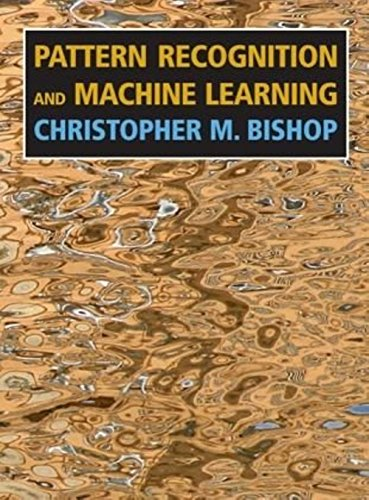
\includegraphics[width=0.25\linewidth]{figs/bishop}
	\caption{The front cover of \cite{bishop_pattern_2011}.}
	\label{fig:duda}
\end{figure}
\end{abstract}

\clearpage

{\small \tableofcontents}


\clearpage
\section{Chapter notes}

Below are some comments on the text.

\begin{easylist}[itemize]
	\ListProperties(Space=\listSpace, Space*=\listSpace, Numbers1=l, FinalMark1={)})
	# Page 306 introduces $\mathsf{t} = (t_1, \ldots, t_N)^{\operatorname{T}}$.
	On the following page $\mathsf{t}_N$ is defined as $(t_1, \ldots, t_N)^{\operatorname{T}}$.
	Perhaps confusingly, both $\mathsf{t}$ and $\mathsf{t}_N$ are used interchangeably after this; but they refer to the same vector.
\end{easylist}



\clearpage

\section{Chapter summaries}

\subsubsection*{Notation}
Scalar data is given by $\mathsf{x} = \left(x_1, \dots, x_N\right)^T$, where $N$ is the number of samples. 
Vector data is given by $\vect{X}$, which has dimensions $N \times M$, where $N$ is the number of data points (rows) and $M$ is the dimensionality of the feature space (columns).

\subsubsection*{Mathematics}
Some useful mathematics is summarized here, also see the book appendix.
\begin{easylist}[itemize]
	\ListProperties(Space=\listSpace, Space*=\listSpace)
	# The \emph{gamma function} $\Gamma(x)$ satisfies $\Gamma(x) = (x-1) \Gamma(x-1)$, and is given by
	\begin{equation*}
	\Gamma(x) = \int_{0}^{\infty} u^{x-1} e^{-u}  \, du.
	\end{equation*}
	It's a ``continuous factorial,'' which is proved by integration by parts and induction.
	
	# The \emph{Jensen inequality} states that, for convex functions
	\begin{equation*}
	f\left( \sum_j \lambda_j x_j\right) \leq \sum_j \lambda_j f(x_j),
	\end{equation*}
	where $\sum_j \lambda_j = 1$ and $\lambda_j \geq 0$ for every $j$.
\end{easylist}

% ----------------------------------------------------------------------------
\subsection{Introduction}


\subsubsection*{Probability}
The joint probability is given by $p(x, y)$, which is short notation for $p(X = x_i \cap Y = y_j)$.
\begin{easylist}[itemize]
	\ListProperties(Space=\listSpace, Space*=\listSpace)
	# The sum rule is 
	\begin{equation*}
	p(x) = \sum_y p(x, y) = \int p(x, y) \, dy.
	\end{equation*}
	## Applying the sum rule as above is called ``marginalizing out $y$.''
	# The product rule is 
	\begin{equation*}
	p(x, y) = p(x | y) p(y).
	\end{equation*}
	## Computing $p(x | y)$ is called ``conditioning on $y$.''
	# Let $\vect{w}$ be parameters and $\D$ be data.
	Bayes theorem is given by
	\begin{equation*}
	p(\vect{w} | \D) = \frac{p(\D | \vect{w}) p(\vect{w})}{p(\D)} \quad \Leftrightarrow \quad
	\text{posterior} = \frac{\text{likelihood} \times \text{prior}}{\text{evidence}}.
	\end{equation*}
	
	## Frequentist: data $\D$ generated from a fixed $\vect{w}$.
	## Bayesian: data $\D$ fixed, find best $\vect{w}$ given this data.
	# Frequentists generally quantify the properties of data driven
	quantities in light of the fixed model parameters,
	while Bayesians generally quantify the properties of unknown
	model parameters in light of observed data.
	See \cite{vanderplas_frequentism_2014}.
\end{easylist}

\subsubsection*{Expectation and covariance}
Let $x$ be distributed with density $p(x)$, then
\begin{easylist}[itemize]
	\ListProperties(Space=\listSpace, Space*=\listSpace)
	# The expectation of a function $f(x)$ defined over $x$ with probability density $p(x)$ is
	\begin{equation*}
	\E[f] = \sum_j f(x_j) p (x_j) = \int f(x) p(x) \, dx
	\end{equation*}
	# The variance of $f(x)$ is
	\begin{equation*}
	\var[f] = \E \left[ (f - \E[f])^2\right] = \E[f^2] - \E[f]^2
	\end{equation*}
	# The covariance of $x$ and $y$ given by
	\begin{equation*}
	\cov[x, y] = \E_{x,y} \left[ (x - \E[x]) (y - \E[y])\right]
	\end{equation*}
	# The covariance matrix $\mathbf{\Sigma}$ has entries $\sigma_{ij}$ corresponding to the covariance of variables $i$ and $j$.
	Thus $\vect{\Sigma} = \vect{I}$ means no covariance.
	(Note that real data may have no covariance and still be dependent, i.e. have predictive power, $x_j = f(x_k)$ where $f$ is non-linear.
	See ``Anscombe's quartet'' on Wikipedia.)
\end{easylist}

\subsubsection*{Polynomial fitting}
Let $y(x, \vect{w}) = \sum_{j = 1}^{M} w_j x^j$ be a polynomial.
We wish to fit this polynomial to values $\sf{x} = \left(x_1, \dots, x_N\right)$ and $\sf{t} = \left(t_1, \dots, t_N\right)$
i.e. a degree $M$ polynomial fitting $N$ data points.

\begin{easylist}[itemize]
	\ListProperties(Space=\listSpace, Space*=\listSpace)
	# The maximum likelihood solution is to minimize
	\begin{equation*}
	E(\vect{w}, \mathsf{x}) \propto \sum_{n = 1}^{N} \left[ y (x_n, \vect{w}) - t_n\right]^2.
	\end{equation*}
	# Regularization adds a weight-dependent error so that $\widetilde{E}(\vect{w}, \mathsf{x}) = E(\vect{w}, \mathsf{x}) + E(\vect{w})$.
	For instance, Ridge minimizes the $2$-norm:
	\begin{equation*}
	\widetilde{E}(\vect{w}, \mathsf{x}) \propto \sum_{n = 1}^{N} \left[ y (x_n, \vect{w}) - t_n\right]^2 + \lambda \norm{\vect{w}}_2^2
	\end{equation*}
	While LASSO (Least Absolute Shrinkage and Selection Operator) minimizes and error with the $1$-norm.
	Both are examples of \emph{Tikhonov regularization}.
\end{easylist}

\subsubsection*{Gaussians}
The multivariate Gaussian is given by
\begin{equation*}
\N\left(x | \vect{\mu}, \vect{\Sigma}\right) = 
\frac{1}{(2\pi)^{D/2} \abs{\vect{\Sigma}}^{1/2}}  
\exp\left( - \frac{1}{2} 
(\vect{x} - \vect{\mu})^T
\vect{\Sigma}^{-1}
(\vect{x} - \vect{\mu})
\right)
\end{equation*}
where $\vect{\mu}$ is the mean and $\vect{\Sigma}$ is the covariance.
Working with the precision $\vect{\Lambda} := \vect{\Sigma}^{-1}$ is sometimes easier.

\subsubsection*{Parameter estimation}
Let $\sf{x} = \left\{x_1, \dots, x_N\right\}$ be a data set which is identically and independently distributed (i.i.d). 
The likelihood function for the Gaussian is
\begin{equation*}
p\left(\sf{x} | \mu, \sigma^2 \right) = 
\prod_{j = 1}^{N} \N \left(x_j | \mu, \sigma^2\right).
\end{equation*}
Estimates for the parameters $\vect{\theta} = (\mu, \sigma^2)$ can be obtained by maximizing the likelihood, which is equivalent to maximizing the log-likelihood $\ln p\left(\sf{x} | \mu, \sigma^2 \right)$.
\begin{easylist}[itemize]
	\ListProperties(Space=\listSpace, Space*=\listSpace)
	# Maximizing the likelihood $p(\D | \vect{w})$ is equivalent to minimizing $E = \vect{e}^T\vect{e}$ in polynomial fitting.
	# Maximizing the posterior $p(\vect{w} | \D)$ (MAP) is equivalent to minimizing regularized sum of squares $E = \vect{e}^T\vect{e} + \lambda \vect{w}^T \vect{w}$.
\end{easylist}


\subsubsection*{Model selection}
\begin{easylist}[itemize]
	\ListProperties(Space=\listSpace, Space*=\listSpace)
	# Both model and model hyperparameters must be determined.
	## Minimize the error over the test set. 
	Balance bias and variance. 
	High bias can lead to underfitting,
	high variance can lead to overfitting.
	# Split data into training, testing and validation.
	# If data is scarce, using $K$-fold cross validation is an option.
\end{easylist}

\subsubsection*{Decision theory}
\begin{easylist}[itemize]
	\ListProperties(Space=\listSpace, Space*=\listSpace)
	# Assign $\vect{x}$ to a region $\Reg_j \subseteq \R^M$ corresponding to a class $\Class_j$, which might or might not be the true class.
	# Minimizing misclassification is done by assigning $\vect{x}$ to the $\Class_j$ which maximizes the posterior $p(\Class_j | \vect{x})$.
	This is equivalent to maximizing chance of begin correct.
	# Loss function $L_{k,j}$ may be used, the loss function assigns a penalty when the true class and the predicted class differ. 
	$L_{k,j} \neq L_{j,k}$ in general.
	Pick the $\Class_j$ which minimizes expected loss, i.e. pick the class $\Class_j$ which minimizes
	\begin{equation*}
	\sum_k L_{k, j} p( \vect{x}, \Class_j).
	\end{equation*}
\end{easylist}
Three general decision approaches in decreasing order of complexity:
(1) inference with class conditional probabilities $p(\vect{x} | \Class_j)$,
(2) inference with posterior class probabilities $p(\Class_j | \vect{x})$ and
(3) discriminant function.
\[\begin{tikzcd}[column sep=6em]
\vect{x} \arrow[]{r}{\text{inference}} 
\arrow[swap, bend right = 20]{rr}{\text{discriminant function}} 
& p(\Class_k , \vect{x}) \arrow[]{r}{\text{decision}} & \Class_k
\end{tikzcd}\]

\subsubsection*{Information theory}
\begin{easylist}[itemize]
	\ListProperties(Space=\listSpace, Space*=\listSpace)
	# $h(x) = - \ln p(x)$ measures the degree of surprise.
	# The entropy is the expected surprised, defined as
	\begin{equation*}
	\H[p] = \E[h] =
	- \sum_j p(x_j) \ln p(x_j)
	=
	 - \int p(x) \ln p(x) \, dx 
	\end{equation*}
	and measures how many nats are needed to encode the optimal transmission of values drawn from $p(x)$.
	## Discrete entropy is maximized by the uniform distribution.
	## Continuous (or differential) entropy is maximized by the Gaussian.
	# Conditional entropy is given by 
	\begin{equation*}
		\H[x|y] = - \sum_{i,j} p(x_i, y_j) \ln p(x_i | y_j)
		= - \iint p(x, y) \ln p(x_i | y_j) \, dx \, dy ,
	\end{equation*}
	and we have that $\H[x, y] = \H[y | x] + \H[x]$.
	
	# The Kullback-Leibner divergence is given by
	\begin{equation*}
	\KL(p \Vert q) = - \int p(x) \ln \left( \frac{q(x)}{p(x)}\right) \, dx
	\end{equation*}
	and is interpreted as the additional information needed if using $q(x)$ to encode values instead of the correct $p(x)$.
\end{easylist}




% ----------------------------------------------------------------------------
\subsection{Probability Distributions}


\subsubsection*{Conjugate priors}
\begin{easylist}[itemize]
	\ListProperties(Space=\listSpace, Space*=\listSpace)
	# Since we know that
	\begin{align*}
	p(\vect{w} | \D) & \propto p(\D | \vect{w}) \times p(\vect{w}) \\
	\text{posterior} & \propto \text{likelihood} \times \text{prior}
	\end{align*}
	we seek probability density functions such that the left hand side and the right hand side is of the same functional form.
	In other words, the likelihood $p(\D | \vect{w})$ is fixed, and we seek priors $p(\vect{w})$ such that posterior $p(\vect{w} | \D)$ is of the same functional form.
	The idea is similar to eigenfunctions.
	
	# Example: 
	Since the binomial distribution is proportional to 
	$p^k (1-p)^{n-k}$, the Beta distribution, proportional to
	$p^{\alpha-1}(1-p)^{\beta-1}$, is a conjugate prior.
	The product of these distributions then ensures that the posterior is of the same functional form as the prior.
\end{easylist}

\begin{center}
	\begin{tabular}{ll} 
		\toprule 
		Parameter & Conjugate prior \\ \midrule
		$\mu$ in Gaussian & Gaussian \\
		$p$ in Binomial & Beta-distribution \\
		$\vect{p}$ in Multinomial & Dirichlet-distribution \\
		\bottomrule
	\end{tabular}
\end{center}


\subsubsection*{The multidimensional Gaussian}
\begin{center}
	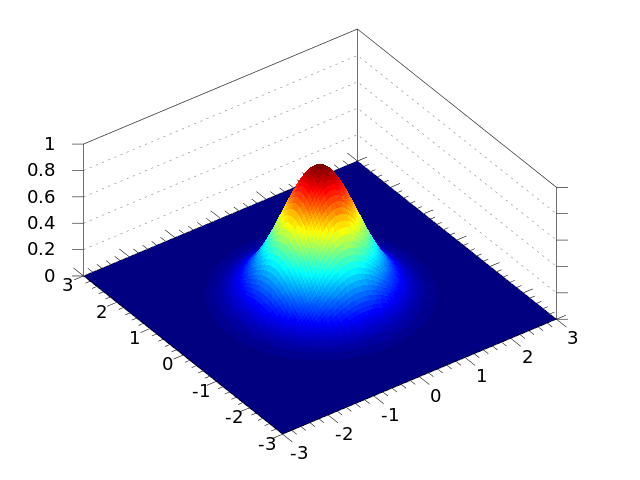
\includegraphics[width=0.6\linewidth]{figs/2d_gaussian}
\end{center}
\begin{easylist}[itemize]
	\ListProperties(Space=\listSpace, Space*=\listSpace)
	# Gaussians arise naturally in sums $x_1 + \dots + x_N$ and averages, since when $N \to \infty$ the sum is normally distributed by the \emph{central limit theorem}.
	# The multidimensional Gaussian can be diagonalized by diagonalizing
	the precision matrix $\vect{\Lambda} = \vect{\Sigma}^{-1}$, then $\exp(\vect{x}^T \vect{\Lambda} \vect{x}) \cong \exp(\vect{y}^T \vect{D} \vect{y})$, where $\vect{D} = \operatorname{diag}(d_1, \dots, d_D)$.
	# One limitation is the unimodal nature of the Gaussian, i.e. it has a single peak.
	
	# \textbf{Partitioned Gaussians.}
	Let $\vect{x} \sim \N (\vect{x} | \vect{\mu}, \vect{\Sigma})$, where $\vect{\Lambda} = \vect{\Sigma}^{-1}$ 
	and 
	\begin{equation*}
	\vect{x} =
	\begin{pmatrix}
	\vect{x}_a \\ 
	\vect{x}_b 
	\end{pmatrix}
	\quad 
	\vect{\mu} =
	\begin{pmatrix}
	\vect{\mu}_a \\ 
	\vect{\mu}_b 
	\end{pmatrix}
	\quad 
	\vect{\Sigma} =
	\begin{pmatrix}
	\vect{\Sigma}_{aa} & \vect{\Sigma}_{ab}  \\ 
	\vect{\Sigma}_{ba} & \vect{\Sigma}_{bb}.\
	\end{pmatrix}.
	\end{equation*}
	## \textbf{Conditional distribution}
	\begin{align*} 
	p(\vect{x}_a |\vect{x}_b )
	&= \N (\vect{x} | \vect{\mu}_{a | b}, \vect{\Lambda}_{aa}^{-1}) \\
	\vect{\mu}_{a | b} &= 
	\vect{\mu}_{a} - \vect{\Lambda}_{aa}^{-1} \vect{\Lambda}_{ab} (\vect{x}_b - \vect{\mu}_b)
	\end{align*}
	
	## \textbf{Marginal distribution}
	\begin{equation*} 
	p(\vect{x}_a  )
	= \N (\vect{x}_a | \vect{\mu}_{a}, \vect{\Sigma}_{aa})
	\end{equation*}
	## These results are proved using inverse of $2 \times 2$ block matrices and examining the quadratic and linear terms in the exponential.
	# There also exist closed-form expressions for Bayes theorem when the prior and likelihood are Gaussians with linear relationship.
\end{easylist}



\subsubsection*{Bayesian inference}
\begin{easylist}[itemize]
	\ListProperties(Space=\listSpace, Space*=\listSpace)
	# Gaussian variables.
	## To estimate $\mu_N$ ($\sigma^2$ is assumed known), use Gaussian prior.
	## To estimate $\lambda = 1/\sigma^2$, use Gamma function as prior, i.e.
	\begin{equation*}
	\operatorname{Gam}(\lambda | a, b) = \frac{b^a \lambda^{a-1}}{\Gamma(a)} \exp (-b \lambda)
	\end{equation*}
	since it has the same functional form as the likelihood.
	# The Student-t distribution may be motivated by:
	## Adding an infinite number of Gaussians with various precisions. 
	## It's the distribution of the sample mean  $(\bar{X} - \mu ) / (S / \sqrt{n})$ when $x_1, \dots, x_N$ are i.d.d. from a Gaussian.
	## As the degrees of freedom $\text{df} \to \infty$, the Student-t distribution converges to a Gaussian.
	An important property of the Student-t distribution is it's \emph{robustness} to outliers.
\end{easylist}

\subsubsection*{Periodic variables}
\begin{easylist}[itemize]
	\ListProperties(Space=\listSpace, Space*=\listSpace)
	# The mean can be measured as $\bar{\theta}$, where we think of the data as lying in a circle.
	# The \emph{von-Mises distribution} is a Gaussian on a periodic domain.
	It is given by
	\begin{equation*}
	p(x | \theta_0, m) = \frac{1}{2 \pi I_0(m)} \exp \left[m \cos (\theta - \theta_0)\right].
	\end{equation*}
\end{easylist}

\subsubsection*{The exponential family}
\begin{easylist}[itemize]
	\ListProperties(Space=\listSpace, Space*=\listSpace)
	# The exponential family is given by
	\begin{equation*}
	p(\vect{x} | \vect{\eta}) =
	g(\vect{\eta})  h (\vect{x}) 
	\exp \left( \vect{\eta}^T u(\vect{x}) \right)
	\end{equation*}
	and many probability functions are members of this family.
	The entries of the vector $\vect{\eta}$ are called \emph{natural parameters}, and $g(\vect{\eta})$ is a normalization constant.
	# Maximum likelihood depends only on the \emph{sufficient statistics} $\sum_n u(\vect{x}_n)$.
	# Non-informative priors make few assumptions,
	letting the data speak for itself.
\end{easylist}

\subsubsection*{Nonparametric methods}
\begin{easylist}[itemize]
	\ListProperties(Space=\listSpace, Space*=\listSpace)
	# The general equation for density estimation is
	\begin{equation*}
	p(\vect{x}) \simeq \frac{K}{NV}
	\end{equation*}
	where $K$ is the number of points in a neighborhood of volume $V$ and $N$ is the total number of points.
	# Kernel functions (or Parzen windows) estimate a neighborhood giving decreasing weight to samples further away, e.g. a Gaussian kernel.
	The volume $V$ is fixed, the data (and kernel function) determines $K$.
	# Nearest neighborhood fixes $K$, letting $V$ be a function of the data.
\end{easylist}

% ----------------------------------------------------------------------------
\subsection{Linear Models for Regression}
\subsection*{Linear basis function models}
\begin{easylist}[itemize]
	\ListProperties(Space=\listSpace, Space*=\listSpace)
	# We assume the dependent data $\vect{y}$ may be written as
	\begin{equation*}
	y(\vect{x}, \vect{w}) = \sum_{j = 0}^{M-1} \vect{w}_j \phi_j(\vect{x}) = \vect{w}^T \vect{\phi}(\vect{x}).
	\end{equation*}
	## The function $y(\vect{x}, \vect{w})$ is linear in $\vect{w}$, but not necessarily in $\vect{x}$ since $\phi_j (\cdot)$ might be a non-linear function.
	It's called a \emph{linear model} because it's linear in $\vect{w}$.
	## Choices for the functions $\{ \phi_j \}$ include identity, powers of $x$, Gaussians, sigmoids, Fourier basis, Wavelet basis, and arbitrary non-linear functions.
	# Assuming a noise term $\epsilon \sim \N(0, \beta^{-1})$, the maximum-likelihood solution is
	\begin{equation*}
	\vect{w}_\text{ML} = \left(\vect{\Phi}^T \vect{\Phi} \right)^{-1} \vect{\Phi}^T \vect{t} = \vect{\Phi}^\dagger \vect{t},
	\end{equation*}
	where $\vect{\Phi}^\dagger$ is the \emph{Moore-Penrose pseudoinverse} and the \emph{design matrix} $\vect{\Phi}$ has entries $\vect{\Phi}_{ij} = \phi_j(\vect{x}_i)$.
	The ML solution is equivalent to minimizing the sum of squares.
	
	# Sequential learning is possible with e.g. the gradient descent algorithm, which is used to compute $\vect{w}^{(\tau + 1)} = \vect{w}^{\tau} - \eta \nabla E_n$.
	This facilitates on-line learning.
	
	# If there are multiple outputs which are linear in the same set of basis functions, the solution is $\vect{w}_k = \vect{\Phi}^\dagger \vect{t}_k$ for every output $k$, and the system decouples.
	
	# Regularizing the error $E(\vect{w})$ with a quadratic term $\alpha \vect{w}^T \vect{w} /2$ has ML solution
	\begin{equation*}
	\left( \alpha \vect{I} + \vect{\Phi}^T \vect{\Phi} \right)
	\vect{w}
	=
	\vect{\Phi}^T \vect{t}.
	\end{equation*}
	The solution above is equivalent to a prior $p(\vect{w} \mid \alpha) = \N (\vect{w} \mid  \vect{0}, \alpha^{-1} \vect{I})$.
\end{easylist}


\subsection*{The Bias-Variance decomposition}
\begin{easylist}[itemize]
	\ListProperties(Space=\listSpace, Space*=\listSpace)
	# The bias-variance decomposition is
	\begin{equation*}
	\text{expected loss} = (\text{bais})^2 + \text{variance} + \text{noise}.
	\end{equation*}
	# Imagine drawing many data sets $\D$ from a distribution $p(t, \vect{x})$.
	## The \textbf{bias} is the distance from the average prediction to the conditional expectation $f(\vect{x}) = \E \left[t | \vect{x} \right]$.
	In other words:
	\begin{equation*}
		\mathrm{Bias}\big[\hat{f}(\vect{x})\big] = \E \big[\hat{f}(\vect{x}) - f(\vect{x})\big]
	\end{equation*}
	## The \textbf{variance} is the variability of $y(\vect{x}; \D)$ around it's average.
	\begin{equation*}
		\mathrm{Var}\big[\hat{f}(\vect{x})\big] = \E [\hat{f}(\vect{x})^2] - \mathrm{E}[{\hat{f}}(\vect{x})]^2
	\end{equation*}
	# Flexible models have high variance, while rigid models have high bias.
\end{easylist}

\subsection*{Bayesian linear regression}
\begin{easylist}[itemize]
	\ListProperties(Space=\listSpace, Space*=\listSpace)
	# We introduce a parameter distribution over $\vect{w}$, for instance an isotropic Gaussian distribution with covariance matrix $\vect{S}_0 = \alpha^{-1} \vect{I}$.
	\begin{equation*}
	p(\vect{w}) = \N (\vect{w} | \vect{m}_0, \vect{S}_0)
	\end{equation*}
	Although the prior $p(\vect{w})$ is isotropic, the posterior $p(\vect{w} \mid \mathsf{t})$ need not be.
	\begin{align*}
	    p(\vect{w}) &= \N ( \vect{w} \mid \vect{m}_0, \vect{S}_0) \quad \tag{prior} \\
	    p(\mathsf{t}\mid \vect{w}) &= \prod_{n=1}^{N} p(t_n \mid \vect{w}) \quad \tag{likelihood} \\
	    p(\vect{w} \mid \mathsf{t}) &= \N ( \vect{w} \mid \vect{m}_N, \vect{S}_N) \quad \tag{posterior} 
	\end{align*}
	
	# Analytical calculations are possible, leading to refinement of the posterior distribution of the parameters $\vect{w}$ as more data is seen.
	
	# A predictive distribution $p(t | \mathsf{t}, \alpha, \beta)$ can be found.
	The predictive distribution accounts for uncertainty of the parameters $\alpha$ and $\beta$.
	
	# The model may be expressed via an \emph{equivalent kernel} $k(x, x_n)$ as 
	\begin{equation*}
		y(\vect{x}, \vect{w}) =
		y(\vect{x}, \vect{m}_N) =
		\beta \vect{\phi} (\vect{x}) \vect{S}_N \vect{\Phi}^T \mathsf{t}
		=
		\sum_{n=1}^{N} \underbrace{
			\beta \vect{\phi} (\vect{x})^T \vect{S}_N \vect{\phi} (\vect{x}_n)
			}_{k(x, x_n)}
			t_n
	\end{equation*}
	In this context, a kernel is a ``similarity function,'' a dot product in some space.
	This can reduce to lower dimensions and make computations faster.
\end{easylist}

\subsection*{Bayestian model selection and limitations}
\begin{easylist}[itemize]
	\ListProperties(Space=\listSpace, Space*=\listSpace)
	# Bayestian model selection uses Bayes theorem with models $\left\{ \mathcal{M}_i \right\}$ and data $\D$ as
	\begin{equation*}
		p( \mathcal{M}_i \mid \D) = \frac{p( \D \mid \mathcal{M}_i) p( \mathcal{M}_i )}{p( \D)}
	\end{equation*}
	where $\mathcal{M}_i$ is a model (distribution).
	It's possible to choose the best model given the data by evaluating the \emph{model evidence} (or \emph{marginal likelihood}) $p( \D \mid \mathcal{M}_i)$ via marginalization over $\vect{w}$.
	
	# Some disadvantages of the simple linear model includes the fact that the functions $\phi_j(\vect{x})$ are fixed before data is observed, and the number of functions often grow exponentially with the number of inputs.
	These shortcomings are often alleviated in other models by the fact that data typically lies on a lower-dimensional manifold.
\end{easylist}

% ----------------------------------------------------------------------------
\subsection{Linear Models for Classification}

\subsection*{Least squares and Fisher's linear discriminant}
\begin{easylist}[itemize]
	\ListProperties(Space=\listSpace, Space*=\listSpace)
	# The following are non-probabilistic models, where the output is not a probability.
	# \emph{Least squares classification} minimizes a quadratic error function, and is analytically tractable.
	The results are not probabilities, the method is very sensitive to outliers, and does not necessarily give good results even when the data is linearly separable.
	# \emph{Fisher's linear discriminant} seeks to find $\vect{w}$ to minimize
	\begin{equation*}
		J(\vect{w}) = 
		\frac{\vect{w}^T \vect{S}_{B} \vect{w}}{\vect{w}^T \vect{S}_{W} \vect{w}}
		= 
		\frac{\text{between class variance}}{\text{within class variance}}.
	\end{equation*}
	The method projects data to a (hopefully) desirable subspace, where generative or discriminative methods may be used.
	Solved by $\vect{w} \propto \vect{S}_{W}^{-1} \left( \vect{m}_2 - \vect{m}_1 \right)$.
	# The \emph{perceptron algorithm} find a separating plane if the data is linearly separable, but does terminate otherwise.
	Historically important.
\end{easylist}

\subsection*{Generalized linear models and probabilistic generative models}
\begin{easylist}[itemize]
	\ListProperties(Space=\listSpace, Space*=\listSpace)
	
	# A \emph{generalized linear model} (GLM) is of the form $y(\vect{x}) = f\left( \vect{w}^T \vect{x} + w_0 \right)$, where the \emph{activation function} $f(\cdot)$ may be non-linear.
		
	# A probabilistic model first models $p(\vect{x} \mid \mathcal{C}_k )$ and $p(\mathcal{C}_k)$, and then uses Bayes theorem to model $p(\mathcal{C}_k \mid \vect{x})$.
	From Bayes theorem, we have
	\begin{equation*}
		p(\mathcal{C}_1 \mid \vect{x})
		=
		\frac{p( \vect{x} \mid \mathcal{C}_1) p(\mathcal{C}_1)}{p( \vect{x} \mid \mathcal{C}_1) p(\mathcal{C}_1) + p( \vect{x} \mid \mathcal{C}_2) p(\mathcal{C}_2)}
		=
		\underbrace{\frac{1}{1 + \exp(-a)}}_{\text{the sigmoid } \sigma(a)},
	\end{equation*}
	where $a = 
	\ln \left( p( \vect{x} \mid \mathcal{C}_1) p(\mathcal{C}_1) \right)
	-
	\ln \left( p( \vect{x} \mid \mathcal{C}_2) p(\mathcal{C}_2) \right)$.
	If we assume normal distributions with shared covariance matrices, then $a(\vect{x})$ is linear in $\vect{x}$.
\end{easylist}

\subsection*{Probabilistic discriminative models}
\begin{easylist}[itemize]
	\ListProperties(Space=\listSpace, Space*=\listSpace)
	# A probabilistic model finds $p(\mathcal{C}_k \mid \vect{x})$ directly, without modeling the class-conditional distribution of $p(\vect{x} \mid \mathcal{C}_k)$.
	In other words, we can determine $\vect{w}$ in the GLM $y(\vect{x}) = f\left( \vect{w}^T \vect{x} + w_0 \right)$ directly.
	This entails fitting $\mathcal{O}(M)$ coefficients instead of $\mathcal{O}(M^2)$.
	
	# To find $\vect{w}$ in $y(\vect{x}) = \sigma \left( \vect{w}^T \vect{x} + w_0 \right)$, we minimize the \emph{cross entropy}, given by the negative log-likelihood
	\begin{equation*}
		E(\vect{w}) = 
		- \ln \underbrace{p(\mathsf{t} \mid \vect{w})}_{\text{likelihood}} =
		- \sum_{n=1}^{M} \underbrace{t_n \ln (y_n) + (1 - t_n) \ln (1 - y_n)}_{\text{cross entropy}}.
	\end{equation*}
	# Using the \emph{Newton-Raphson} method
	\begin{equation*}
		\vect{w}^{n+1}
		=
		\vect{w}^{n} - \vect{H}^{-1}(\vect{w}^{n}) \nabla E (\vect{w}^{n})
	\end{equation*}
	on the error function $E(\vect{w})$ is an instance of the \emph{iterative reweighed least squares} (IRLS) method.
	Every step involves a weighted least squares problem, and $E(\vect{w})$ has a unique global minimum.
\end{easylist}

\subsection*{The Laplace approximation}
\begin{easylist}[itemize]
	\ListProperties(Space=\listSpace, Space*=\listSpace)
	# The idea behind the \emph{Laplace approximation} is to place a normal distribution on a mode $\vect{z}_0$ of the function $f(\vect{z})$
	\begin{equation*}
		f(\vect{z}) \simeq f(\vect{z}_0) \exp \left[ 
		- \frac{1}{2}
		(\vect{z} - \vect{z}_0)^T \vect{A}
		(\vect{z} - \vect{z}_0)
		 \right]
		 \qquad
		 \vect{A} = \left. - \nabla \nabla \ln f(\vect{z}) \right|_{\vect{z} = \vect{z}_0}
	\end{equation*}
	# One application of Laplace approximation is Bayesian logistic regression, which is generally intractable.
	Using the Laplace approximation, an approximation to exact Bayesian inference is possible.
\end{easylist}

% ----------------------------------------------------------------------------
\subsection{Neural networks}
\subsection*{The basic idea of neural networks}
\begin{easylist}[itemize]
	\ListProperties(Space=\listSpace, Space*=\listSpace)
	# A neural network has a fixed number of adaptable basis functions.
	Unlike the algorithms considered so far, neural networks let the \emph{activation functions} themselves be learned, not just the weights of their linear combinations. The notation is:
	\begin{equation*}
	\begin{tikzcd}
	x_i, \, i=1,\ldots, D \arrow{r}{w_{ji}^{\text{(1)}}}
	\arrow[bend left = 20]{rr}{w_{ki}^{\text{(3)}}}
	&  
	z_j , \, j=1,\ldots, M \arrow{r}{w_{kj}^{\text{(2)}}} & 
	y_k , \, k=1,\ldots, K
	\end{tikzcd}
	\end{equation*}
	
	# In a two-layer network, the equation for the output is
	\begin{equation*}
		y_k = \sigma \bigg( 
		\sum_{j=0}^{M} w_{kj}^{(2)}
		h 
		\bigg( 
		\underbrace{\sum_{i=0}^{M} w_{ji}^{(1)} x_i}_{z_j}
		 \bigg)
		 \bigg),
	\end{equation*}
	where $\sigma(\cdot)$ and $h(\cdot)$ are the activation functions in the final (3rd) and hidden (2nd) layer, respectively.
	They may differ in general.
	## In regression problems, the final activation function $\sigma(\cdot)$ is often the identity, and the error $E(\vect{w})$ is the sum-of-squares error.
	## In regression problems, the final activation function $\sigma(\cdot)$ is often the softmax, and the error $E(\vect{w})$ is the cross entropy.
	# To see how the first layer learns activation functions, consider a $D$-$D$-$2$ network with softmax activation functions trained using cross entropy error.
	The first part of the network learns non-linear functions $\phi_j(\vect{x})$, which are used for logistic regression in the second part.
	This is perhaps best seen if we write
	\begin{equation*}
		y_k = \sigma \bigg( 
		\sum_{j=0}^{D} w_{kj}^{(2)}
		\phi_j(\vect{x})
		\bigg),
		\quad 
		 \quad
		\phi_j(\vect{x})
		=
		h 
		\bigg( 
		\sum_{i=0}^{D} w_{ji}^{(1)} x_i
		\bigg).
	\end{equation*}
	
	
\end{easylist}

\subsection*{Network training}
\begin{easylist}[itemize]
	\ListProperties(Space=\listSpace, Space*=\listSpace)
	# Network training involves finding weights $\vect{w}$ to minimize $E(\vect{w})$, this is a non-convex optimization problem, typically solved iteratively, i.e.
	\begin{equation*}
		\vect{w}^{k+1} = \vect{w}^{k} + \Delta  \vect{w}^{k}
	\end{equation*}
	where $\Delta  \vect{w}^{k}$ is some update rule. 
	For instance $\Delta  \vect{w}^{k} = - \eta \nabla E \left( \vect{w}^{k} \right)$ for gradient descent, which requires gradient information.
	
	# Computing the gradient $\nabla_{\vect{w}} E \left( \vect{w}^{k} \right)$ is done using back-propagation, which is application of the chain rule of calculus to the network.
	First information is propagated forward in the network, then an error is computed and the $\partial_{w_{jk}} E$ are found by propagating information backward in the network.
	
	# Second order derivatives, i.e. the Hessian $\vect{H} = \nabla \nabla E$, may be approximated or computed.
	Approximation schemes include diagonal approximation, outer product approximation, inverse from outer product (using the Woodbury matrix identity) and finite differences.
	Exact evaluation is also possible, and computing fast multiplication is possible by considering the operator $\mathcal{R}\{\cdot \}$ in $\vect{v}^T \vect{H} = \vect{v}^T \nabla \nabla E =\mathcal{R}\{ \nabla E \}$.
\end{easylist}


\subsection*{Neural network regularization}
\begin{easylist}[itemize]
	\ListProperties(Space=\listSpace, Space*=\listSpace)
	# Naively adding a regularization term such as $\widetilde{E}(\vect{w} = E(\vect{w}) + \alpha \vect{w}^T \vect{w}/2$ will be inconsistent with scaling properties.
	A better regularization is to use
	\begin{equation*}
		\frac{\alpha_1}{2} \sum_{w \in \mathcal{W}_1} w^2
		+
		\frac{\alpha_2}{2} \sum_{w \in \mathcal{W}_2} w^2
	\end{equation*}
	where $\mathcal{W}_1$ denotes (non-bias) weights in layer 1.
	## The regularization above is called \emph{weight-decay}, since it corresponds to decaying weights while training by multiplying with a factor between 0 and 1. 
	It can be shown that
	\begin{equation*}
		\text{weight decay} \cong \text{early stopping}.
	\end{equation*}
	
	# Four ways to learn invariance is
	## \textbf{Augmenting the training data while learning}, using some function $\vect{s}(\vect{x}, \xi)$, where $\vect{s}(\vect{x}, 0) = \vect{x}$.
	As an example, the function might rotate an image slightly.
	## Use \textbf{tangent propagation regularization} to penalize the Jacobian of the neural network, with no penalization along the tangent of the transformation.
	## \textbf{Pre-process} the data and extract invariant features by hand.
	## \textbf{Build invariance into the structure} of the neural net, e.g. CNNs.
	## It can be shown that 
	\begin{equation*}
	\text{augmenting data while learning} \cong \text{tangent propagation regularizer}.
	\end{equation*}
\end{easylist}

\subsection*{Soft weight sharing and mixture density networks}
\begin{easylist}[itemize]
	\ListProperties(Space=\listSpace, Space*=\listSpace)
	# Using \emph{soft weight sharing}, we assume a Gausian mixture distribution as a prior over the weights in the network.
	# \emph{Mixture density networks} work well for \emph{inverse problems}, where $p(t \mid \vect{x})$ might be multimodal.
	The approach is to use a neural network to learn $\pi_k$, $\vect{\mu}_k$ and $\sigma_k^2$ in the mixture density
	\begin{equation*}
		p(t \mid \vect{x}) = \sum_{k=1}^{K} \pi_k 
		\N \left( t \mid \vect{\mu}_k(\vect{x}), \vect{I} \sigma^2_k(\vect{x}) \right).
	\end{equation*}
	The $\{\pi_k\}$ have softmax activations in the output to enforce the summation constraint, while the $\{ \sigma^2_k(\vect{x}) \}$ have exponential activations to enforce positivity.
	
	# A full Bayesian treatment of neural networks is not analytically intractable.
	However, using the Laplace approximation for the posterior parameter distribution, and alternative re-estimation of $\alpha$ and $\beta$ it is possible to use approximate evidence approximation.
\end{easylist}



% ----------------------------------------------------------------------------
\subsection{Kernel methods}
\subsection*{Introduction to kernel methods}
\begin{easylist}[itemize]
	\ListProperties(Space=\listSpace, Space*=\listSpace)
	# The \emph{dual representation} expresses a prediction $y(\vect{x}) = \vect{w}^T \vect{\phi}(\vect{x})$ entirely in terms of the $N$ seen data points by use of the \emph{kernel} $k(\vect{x}, \vect{x}') = \vect{\phi}(\vect{x})^T \vect{\phi}(\vect{x})$.
	This is in contrast to learning weights $\vect{w}$.
	The dual formulation of Ride regression is
	\begin{equation}
	\label{eqn:linear_reg_dual}
		y(\vect{x}) = \vect{k}(\vect{x})^T \left( \vect{K} + \lambda \vect{I} \right)^{-1} \mathsf{t},
	\end{equation}
	where $\vect{k}(\vect{x})^T = 
	(k(\vect{x}_1, \vect{x}),
	k(\vect{x}_2, \vect{x}),
	\ldots,
	k(\vect{x}_N, \vect{x}))$
	and $\vect{K}_{nm} = k(\vect{x}_n, \vect{x}_m)$.
	## Typically the number of data points $N$ is much greater than the dimensionality $M$ of the features $\vect{\phi}(\vect{x})$.
	Since \eqref{eqn:linear_reg_dual} needs to invert $\vect{K} \in \R^{N \times N}$, it's not obviously useful.
	One advantage is that infinite dimensional feature mappings need not be computed explicitly.
	A simple example is 
	$\vect{\phi}(x) = (1, x, x^2, \ldots)$, which is infinite dimensional, but $k(x, x')$ becomes $(1 - x^2)^{-1}$. 
	## A kernel is valid if it corresponds to an inner product a feature space.
	A kernel is valid if $\vect{K}$ is positive definite for every possible $\vect{x}$.
	Valid kernels may be constructed from other valid kernels, for instance
	\begin{equation*}
		k = k_1 + k_2, \qquad k = k_1 k_2, \qquad k = \exp(k_1), \qquad \ldots
	\end{equation*}
	This is called \emph{kernel engineering}.
	# \emph{Kernel regression} (the \emph{Nadaraya-Watson} model) models $p(\vect{x}, t)$ as
	\begin{equation*}
		p(\vect{x}, t) = \frac{1}{N} \sum_{n=1}^{N} f(\vect{x} - \vect{x}_n, t- t_n).
	\end{equation*}
\end{easylist}

\subsection*{Gaussian processes}
\begin{easylist}[itemize]
	\ListProperties(Space=\listSpace, Space*=\listSpace)
	# A prior over weights $\vect{w} \sim p(\vect{w})$, implicitly defines a distribution over functions $y(\vect{x}) = \vect{w}^T \vect{\phi}(\vect{x})$.
	Predictions on a finite set of values is given by $\mathsf{y} = \vect{\Phi} \vect{w}$.
	Formulated in term of kernels, a \emph{Gaussian process} is specified by
	\begin{equation*}
		\E \left[ y(\vect{x}_n) y(\vect{x}_m) \right]
		=
		k(\vect{x}_n, \vect{x}_m)
		= \cov \left[ \mathsf{y} \right].
	\end{equation*}
	# The kernel may for instance be given by
	\begin{equation*}
		k(\vect{x}_n, \vect{x}_m \mid \vect{\theta})
		=
		\phi_0 \exp \left( - \frac{\theta_1}{2}
		\norm{\vect{x}_n - \vect{x}_m} \right)
		+
		\theta_2
		+\theta_3 \vect{x}_n^T \vect{x}_m.
	\end{equation*}
	If $\vect{x}_n \approx \vect{x}_m$, then the kernel will be comparatively large and the covariance will be larger.
	In other words; points that are close are more highly correlated.
	
	\begin{figure}[ht!]
		\centering
		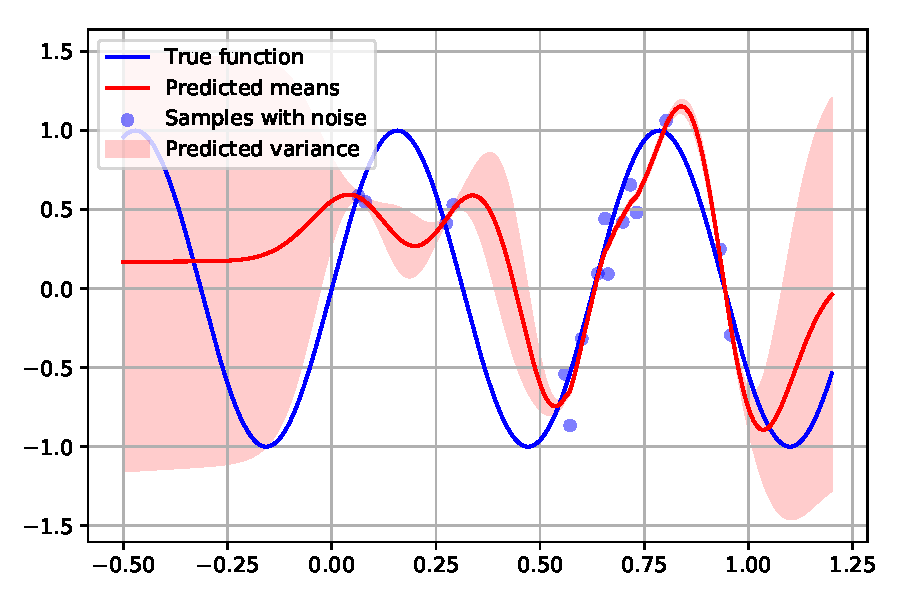
\includegraphics[width=0.7\linewidth]{figs/gaussian_process_regression}
		\caption{Gaussian process regression on data from $y_i = \sin(x_i) + \epsilon$.}
		\label{fig:gaussian_process_regression}
	\end{figure}
	
	
	# In \emph{Gaussian process regression}, the predicted mean and variance is given by
	\begin{align*}
		\mu (X_{N+1}) &= \vect{k}^T \vect{C}_N^{-1} \mathsf{t} \\
		\sigma^2 (X_{N+1}) &= c - \vect{k}^T \vect{C}_N^{-1} \vect{k},
	\end{align*}
	where $\vect{C}_N = k(\vect{x}_n, \vect{x}_m) + \beta^{-1} \delta_{nm}$ is the covariance matrix after observing $N$ points.
\end{easylist}



\subsection*{Hyperparameters and extensions}
\begin{easylist}[itemize]
	\ListProperties(Space=\listSpace, Space*=\listSpace)
	# Hyperparameters $\vect{\theta}$ in $k(\vect{x}_n, \vect{x}_m \mid \vect{\theta})$ can be optimized by maximizing the log likelihood $\ln p (\mathsf{t} \mid \vect{\theta})$, which is in general non-convex.
	This is type 2 maximum likelihood.
	# Gaussian processes can be used for classification, by composing the output with a sigmoid so that $y = \sigma (\vect{a}(\vect{x}))$.
	Not analytically tractable, but approximate methods exist: (1) variational inference, (2) expectation maximization and (3) Laplace approximation.
\end{easylist}

% ----------------------------------------------------------------------------
\subsection{Sparse Kernel Machines}


\subsection*{Support vector machines}

	\begin{figure}[ht!]
		\centering
		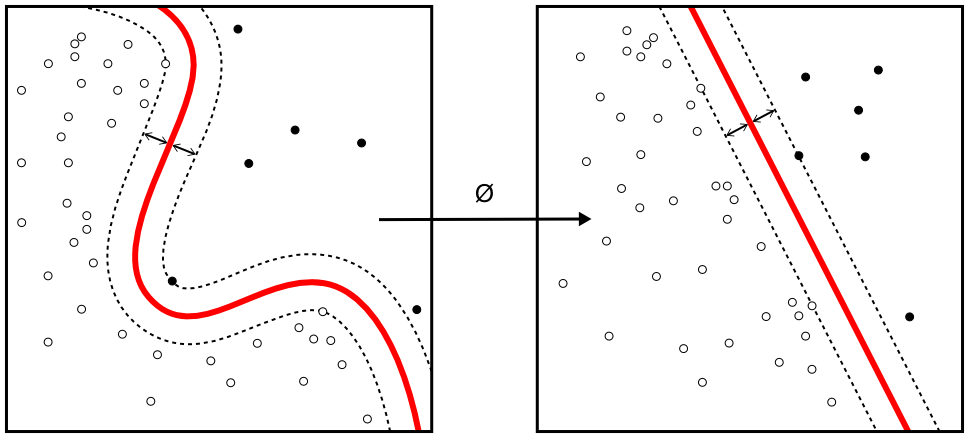
\includegraphics[width=0.7\linewidth]{figs/Kernel_Machine.png}
		\caption{Data which is linearly separable in the feature vector space $\vect{\phi}(\vect{x})$, but not in $\vect{x}$-space.
			The maximum margin hyperplane is non-linear in $\vect{x}$-space.
			Source: Wikipedia.}
		\label{fig:Kernel_Machine}
	\end{figure}
	
\begin{easylist}[itemize]
	\ListProperties(Space=\listSpace, Space*=\listSpace)
	# The main idea (when data is linearly separable) is to optimize $\vect{w}$ and $b$ in the equation $y(\vect{x}) = \vect{w}^T \vect{\phi} (\vect{x}) + b$ so that the separating hyperplane has a maximal margin.
	The points closest to the margin are called \emph{support vectors}, and the hyperplane depends only on these points.
	
	# Lagrange multipliers and the Karush-Kuhn-Tucker (KKT) conditions are needed to solve the problem.
	For the problem below, the Lagrangian is $L(\vect{x}, \lambda) = f(\vect{x}) - \lambda g(\vect{x})$.
	\begin{alignat*}{3}
	\text{Optimization problem} & & \qquad\qquad \text{KKT-conditions}\\
		\operatorname{minimize} & \quad f(\vect{x})& \qquad\qquad g(\vect{x}) \geq 0, \lambda \geq 0 \\
		\text{subject to}  &  \quad g(\vect{x}) \geq 0 & \qquad\qquad \lambda g(\vect{x}) = 0
	\end{alignat*}
	The KKT conditions must be true at the optimum.
	They state that each constraint is either \emph{active} or \emph{inactive}, and generalize Lagrange multipliers to deal with inequality constraints.
	
	# The \textbf{linearly separable classification problem} has Lagrange function
	\begin{equation*}
		L(\vect{w}, b, \vect{a}) = \frac{1}{2} \norm{\vect{w}}^2 - \sum_{n=1}^{N} a_n \left( t_n y_n - 1 \right).
	\end{equation*}
	Differentiating with respect to $\vect{w}$ and $b$, and substituting back into the Lagrange function yields the \emph{dual form} of the optimization problem
	\begin{equation}
	\label{eqn:SVM_dual}
	\widehat{L}(\vect{a}) = \sum_{n=1}^{N} a_n -
	\frac{1}{2}
	\sum_{n=1}^{N} \sum_{m=1}^{N} a_n a_m t_n t_m k(\vect{x}_n, \vect{x}_m)
	\end{equation}
	which is expressed entirely in terms of the kernel $k(\vect{x}_n, \vect{x}_m)$ and the lagrange multipliers. 
	The constraints are $a_n \geq 0$ and $\sum_{n} a_n t_n = 0$, and predictions are given by $y(\vect{x}) = \sum_n  a_n  t_n  k(\vect{x}_n, \vect{x}) + b$.
	Since $a_n = 0$ when point $n$ is not a support vector (the constraint is \emph{inactive}), prediction relies only on the support vectors.
	
	# The \textbf{linearly inseparable classification problem} minimizes
	\begin{equation*}
	C \sum_{n=1}^{N} \xi_n + \frac{1}{2} \norm{\vect{w}}^2, 
	\end{equation*}
	where $\xi_n$ are \emph{slack variables} and the constraint is $t_n y_n \geq 1 - \xi_n$ instead of $t_n y_n \geq 1$.
	The dual Lagrangian function $\widehat{L}(\vect{a})$ is exactly equal to Equation \eqref{eqn:SVM_dual}, but the constraints are now $ 0 \leq a_n \leq C$ (\emph{box constraints}) and $\sum_{n} a_n t_n = 0$.
	
	# The optimization problems above are quadratic programs (QP), and specialized methods for solving QP for SVMs exist: chunking, decomposition methods and sequential minimal optimization.
	The problems are often large, since $k(\vect{x}_n, \vect{x}_m)$ must be evaluated for every pair of points.
	
	# The \textbf{regression problem} introduces a more robust error function
	\begin{equation*}
		\frac{1}{2} \sum_n (y_n - t_n)^2 + \frac{\lambda}{2} \norm{\vect{w}}^2
		\quad 
		\leftrightarrows
		\quad
		C \sum_n E_\epsilon \left( y_n - t_n \right) + \frac{1}{2} \norm{\vect{w}}^2,
	\end{equation*}
	where $E_\epsilon(\cdot)$ increases linearly outside of a margin of width $2\epsilon$.
	Two slack variables $\xi_n \geq 0$ and $\widehat{\xi}_n \geq 0$ are introduced, and minimizing the above is equivalent to
	\begin{equation*}
	 \underset{\vect{\xi}, \vect{\widehat{\xi}}, \vect{w}}{\operatorname{minimize}} \quad 
	C \sum_n (\xi_n + \widehat{\xi}_n) + \frac{1}{2} \norm{\vect{w}}^2,
	\end{equation*}
	 and $\widehat{L}(\vect{a}, \widehat{\vect{a}})$ is again quadratic.
	 The resulting optimization problem is a QP.
	 
	 # The $\nu$-SVM is mathematically equivalent to the above, but uses a parameter $\nu$ which controls the fraction of the data points that become support vectors.
	 This is a more intuitive parameterization.
\end{easylist}

\subsection*{Relevance vector machines}
\begin{easylist}[itemize]
	\ListProperties(Space=\listSpace, Space*=\listSpace)
	# For regression, the model and prior are formulated as
	\begin{align*}
		p(t \mid \vect{x}, \vect{w}, \beta) &= \N (t \mid y (\vect{x}, \vect{w}), \beta^{-1}),
		\quad
		\text{where } y(\vect{x}, \vect{w}) = \sum_n w_n k(\vect{x}_n, \vect{x}) + b \\
		p(\vect{w} \mid \vect{\alpha}) &= \prod_{i}^{M} \N (w_i \mid 0 , \alpha^{-1}_i).
	\end{align*}
	The name \emph{relevance vector machine} comes from the fact that automatic relevance determination is used to infer the important data points in an SVM-like function $y(\vect{x}, \vect{w})$, and these \emph{relevance vectors} are analogous to support vectors.
	
	
	# The hyperparameters $\{\alpha_i \}$ and $\beta$ are efficiently determined through re-estimation equations.
	The expectation maximization algorithm is also an option.
	
	# The model is typically very sparse, even more sparse than SVM, as many of the $\{\alpha_i \}$ are driven to infinity.
	The downside is that the optimization problem is non-convex, and in general takes $\mathcal{O}(M^3)$ time, where $M= N+1$ if a SVM-like kernel is used.
	For classification, Laplace approximation may be used to derive results.
\end{easylist}

% ----------------------------------------------------------------------------
\subsection{Graphical Models}

\begin{figure}[ht!]
	\centering
	\tikz{ %
		
		% Bottom row
		\node[const] (var) {$\sigma^2$} ; %
		\node[latent, right=of var] (that) {$\widehat{t}$} ; %
		\edge {var} {that} ; %
		\node[latent, right=of that] (xhat) {$\widehat{x}$} ; %
		\edge {xhat} {that} ; %
		
		% Middle row
		\node[obs, above=of var, yshift=.19cm] (tn) {$t_n$} ; %
		\node[latent, above=of that] (w) {$\vect{w}$} ; %
		\edge {w} {tn} ; %
		\edge {w} {that} ; %
		\edge {var} {tn} ; %
		
		% Top row
		\node[latent, above=of tn] (x) {$x_n$} ; %
		\node[const, above=of w, yshift=.25cm] (alpha) {$\alpha$} ; %
		\edge {x} {tn} ; %
		\edge {alpha} {w} ; %
		
		% Plate
		\plate[inner sep=0.35cm] {plate1} {(x) (tn)} {N}; %
	}
	\label{fig:graphical_model_regression}
	\caption{A graphical model for polynomial regression.
		Model parameters are shown without circles (e.g. $\sigma^2$), random variables are encircled (e.g. $x_n$), observed random variables are shaded (e.g. $t_n$) and \emph{plate notation} is used to repeat the enclosed nodes.}
\end{figure}

\subsection*{Directed graphs}
\begin{easylist}[itemize]
	\ListProperties(Space=\listSpace, Space*=\listSpace)
	# A \emph{graph} is associated with a factorization of the joint probability density function $p(\vect{x})$.
	For instance, the graph below means that $p(\vect{x})$ can be factored as $p(x_1 \mid x_2) p(x_2) p(x_3 \mid x_2)$.
	It imposes structure on $p(\vect{x})$ by it's \emph{lack} of edges.
	\begin{figure}[ht!]
		\centering
		\tikz{
			\node[latent] (x1) {$x_1$} ; %
			\node[latent, right=of x1] (x2) {$x_2$} ; %
			\node[latent, right=of x2] (x3) {$x_3$} ; %
			\edge {x2} {x1} ; %
			\edge {x2} {x3} ; %
		}
	\end{figure}
	# Approaches to reducing the number of model parameters include:
	## Removing edges: induces factorization properties on $p(\vect{x})$.
	## Sharing parameters: merging parents together into a common node.
	## Restricting the functional form: for instance assuming $p(y=1\mid \vect{x}) = \sigma \left( \vect{w}^T \vect{x} \right)$.

# The three examples below demonstrate \emph{conditional independence properties} in simple directed graphs.
Observing $c$ blocks the \emph{tail-to-tail} and \emph{head-to-tail} paths, but observing $c$ (or any descendant of $c$) unblocks the \emph{head-to-head} path.
\begin{figure}[!htb]
	\centering
	\minipage{0.32\textwidth}
	\tikz{
		\node[latent] (x1) {$a$} ; %
		\node[latent, right=of x1] (x2) {$c$} ; %
		\node[latent, right=of x2] (x3) {$b$} ; %
		\edge {x2} {x1} ; %
		\edge {x2} {x3} ; %
	}
	\begin{align*}
	a \nbigCI b &\mid \emptyset
	\end{align*}
	\tikz{	
		\node[latent, below=of x1] (a) {$a$} ; %
		\node[obs, right=of a] (b) {$c$} ; %
		\node[latent, right=of b] (c) {$b$} ; %
		\edge {b} {a} ; %
		\edge {b} {c} ; %
	}
	\begin{align*}
		a \bigCI b &\mid c
	\end{align*}
	\endminipage
	\minipage{0.32\textwidth}
	\tikz{
		\node[latent] (x1) {$a$} ; %
		\node[latent, right=of x1] (x2) {$c$} ; %
		\node[latent, right=of x2] (x3) {$b$} ; %
		\edge {x1} {x2} ; %
		\edge {x2} {x3} ; %
	}
	\begin{align*}
		a \nbigCI b &\mid \emptyset
	\end{align*}
	
	\tikz{
		\node[latent] (x1) {$a$} ; %
		\node[obs, right=of x1] (x2) {$c$} ; %
		\node[latent, right=of x2] (x3) {$b$} ; %
		\edge {x1} {x2} ; %
		\edge {x2} {x3} ; %
	}
	\begin{align*}
	a \bigCI b &\mid c
	\end{align*}
	\endminipage
	\minipage{0.32\textwidth}%
	\tikz{
		\node[latent] (x1) {$a$} ; %
		\node[latent, right=of x1] (x2) {$c$} ; %
		\node[latent, right=of x2] (x3) {$b$} ; %
		\edge {x1} {x2} ; %
		\edge {x3} {x2} ; %
	}
	\begin{align*}
	a \bigCI b &\mid \emptyset 
	\end{align*}
	\tikz{
		\node[latent] (x1) {$a$} ; %
		\node[obs, right=of x1] (x2) {$c$} ; %
		\node[latent, right=of x2] (x3) {$b$} ; %
		\edge {x1} {x2} ; %
		\edge {x3} {x2} ; %
	}
	\begin{align*}
	a \nbigCI b &\mid c
	\end{align*}
	\endminipage
\end{figure}

# \emph{D-separation}. Consider disjoint subsets $A$, $B$ and $C$ of edges in a graph. 
Let $C$ be observed.
A path from $A$ to $B$ is said to be blocked if
\begin{easylist}[itemize]
	\ListProperties(Space=\listSpace, Space*=\listSpace)
## There is a tail-to-tail or head-to-tail path with a node in $C$ in the path.
## There is a head-to-head path, where the middle not is not in $C$, nor any of it's descendants.
\end{easylist}
If \emph{every} path from $A$ to $B$ is blocked, then $A \bigCI B \mid C$.

# A graph can be thought of as a \emph{filter}.
The filter inputs are pdfs $p(\vect{x})$, and those factoring according to the given graph structure pass through the filter.
For instance, $p(\vect{x}) = \prod_{i} p(x_i)$ would pass any such filter.
The set $\mathcal{DF}$, for \emph{directed factorization}, is the set of probability density functions passing through a specific filter.

# The \emph{Markov blanket} of a graph is the minimal set of nodes that isolates $x_i$ from the rest of the graph.
In other words, $p( x_i \mid x_{\{ i \neq i\}})$ is only functionally dependent on the nodes in the Markov blanket, which consists of parents, children and co-parents when the graph is directed.
\begin{equation*}
	\begin{tikzcd}
	  & x \arrow{dr} &   & x \arrow{dl} &    \\
	x  \arrow{dr} &   & x_i \arrow{dr} \arrow{dl} &   & x \arrow{dl} \\
	  & x &   & x &  
	\end{tikzcd}
\end{equation*}
The Markov blanket in an undirected graph has a similar, but simpler structure; it only consists of the parents and children.
\end{easylist}

\subsection*{Markov random fields}
\begin{easylist}[itemize]
	\ListProperties(Space=\listSpace, Space*=\listSpace)
	# \emph{Markov random fields} are undirected graphs whose nodes are random variables.
	# Sets of nodes $A$ and $B$ are conditionally independent given $C$, denoted $A \bigCI B \mid C$, if removing the nodes in $C$ leaves no path from $A$ to $B$.
	This is simpler than in the directed case, where d-separation and path blocking is more nuanced. 
	# The factors in the factorization of $p(\vect{x})$ are functions of the maximal \emph{cliques} in the graph.
	Cliques are subsets of nodes which are fully connected.
	Let $\vect{x}_C$ be nodes associated with a clique $C$, then
	\begin{equation*}
		\underbrace{\psi_C (\vect{x}_C)}_{\text{potential function}} = \underbrace{ \exp \big(- \underbrace{E(\vect{x}_C)}_{\text{energy function}} \big)}_{\text{Boltzmann distribution}}
	\end{equation*}
	is the \emph{potential function} associated with a clique.
	The joint distribution is given by
	\begin{equation*}
		p(\vect{x}) = \frac{1}{Z} \prod_{C} \psi_C (\vect{x}_C),
	\end{equation*}
	where $Z$ is a normalization constant called the \emph{partition function}.
	
	# A directed graph can be related to an undirected graph by \emph{moralization}.
	This involves ``marrying the parents'' and converting directed edges to undirected edges. 
	It represents a loss of structure.
\end{easylist}

\subsection*{Inference}
\begin{easylist}[itemize]
	\ListProperties(Space=\listSpace, Space*=\listSpace)
	# Inference on a \emph{chain} is accomplished by sending \emph{messages}; one forward and one backward.
	This let's us evaluate marginals $p(x_n)$ efficiently.
	If each variable has $K$ possible states, the algorithm is $\mathcal{O}(NK^2)$ instead of the naive $\mathcal{O}(K^N)$.
	\begin{equation*}
		\begin{tikzcd}
		x_1 \arrow{r} & x_2 \arrow{r} & \ldots \arrow{r} & x_N
		\end{tikzcd}
	\end{equation*}
	
	# \emph{Factor graphs} comprise factor nodes and variable nodes.
	They can be constructed from undirected trees, directed trees and directed polytrees.
	A factor graph is bipartite, and they are used in the sum product algorithm.
	# The \emph{sum-product algorithm} facilitates efficient computation of marginals $p(\vect{x}_s)$ in factor graphs.
	It works by sending messages $\mu_{f \to x}(x)$ and $\mu_{x \to f}(x)$ from leaves to an arbitrary root note, then back to the leaves.
	Marginals are then computed as
	\begin{equation*}
		p(x) = \prod_{s \in \operatorname{ne}(x)} \mu_{f_s \to x}(x).
	\end{equation*}
	# The \emph{max-sum} algorithm finds the state $\vect{x}^{\operatorname{max}}$ maximizing the joint probability function, as well as the value $p(\vect{x}^{\operatorname{max}})$.
	The algorithm involves first sending messages from leaves to root, then \emph{backtracking} to find the state $\vect{x}^{\operatorname{max}}$.
\end{easylist}

% ----------------------------------------------------------------------------
\subsection{Mixture Models and EM}


\subsection*{$K$-means and mixtures of Gaussians}
\begin{easylist}[itemize]
	\ListProperties(Space=\listSpace, Space*=\listSpace)
	# In $K$-means classification, the EM algorithm minimizes the objective function
	\begin{equation*}
		J = \sum_{n=1}^{N} \sum_{k=1}^{K} r_{nk} \norm{\vect{x}_n - \vect{\mu}_k}^2.
	\end{equation*}
	## The \textbf{expectation step} re-assigns points $\vect{x}_n$ to clusters via $r_{nk} \in \{0, 1\}^K$.
	## The \textbf{maximization step} re-computes the $k$ prototypes $\{ \vect{\mu}_k \}$.
	
	# \emph{Mixtures of Gaussians} are given by the equation
	\begin{equation*}
		p(\vect{x}) = \sum_{k=1}^{K} \pi_k \N (\vect{x} \mid \vect{\mu}_k, \vect{\Sigma}_k)
	\end{equation*}
	where $\pi_k$ are the \emph{mixing coefficients}.
	If $p(z_{k} = 1) = \pi_k$, we obtain the model below.
	For every $\vect{x}_n$, there is a latent (unobserved) $\vect{z}_n$ corresponding to which mixture $\vect{x}_n$ is from.
	For instance, if $\vect{z}_n = (0, 1, \ldots)$, then $\vect{x}_n$ is drawn from mixture number $2$.
	
	\begin{center}
		\tikz{
			% Random variables
			\node[latent] (z) {$\vect{z}_n$} ; %
			\node[obs, below=of z] (x) {$\vect{x}_n$} ; %
			\edge {z} {x} ; %
			\plate[inner sep=0.35cm] {plate1} {(x) (z)} {N}; %
			
			% Parameters
			\node[const, left=of z] (pi) {$\pi_k$} ; %
			\node[const, left=of x] (musig) {$\vect{\mu}_k, \vect{\Sigma}_k$} ; %
			\edge {pi} {z} ; %
			\edge {musig} {x} ; %
			\plate[inner sep=0.35cm] {plate1} {(pi) (musig)} {K}; %
		}
	\end{center}
		## The EM algorithm for Gaussian mixtures is the following.
		### The \textbf{expectation step} evaluates the \emph{responsibilities} $\gamma(z_{nk})$, defined as the posterior probabilities $\gamma(z_{nk}) := p(z_{nk} = 1 \mid \vect{x}_n)$.
		### The \textbf{maximization step} re-computes the $\pi_k, \vect{\mu}_k, \vect{\Sigma}_k$ (functions of $\gamma(z_{nk})$).

	
\end{easylist}


\subsection*{The expectation-maximization (EM) algorithm}
\begin{easylist}[itemize]
	\ListProperties(Space=\listSpace, Space*=\listSpace)
	# The goal is to maximize the log likelihood $\ln p(\vect{X} \mid \vect{\theta})$.
	If this is difficult, but maximizing $\ln p(\vect{X}, \vect{Z} \mid \vect{\theta})$ is easier, then the EM algorithm is applicable.
	## The \textbf{expectation step} evaluates the posterior probability of the latent variables $\vect{Z}$ given $\vect{X}$ and $\vect{\theta}^{\text{old}}$.
	These are the responsibilities denoted by $\gamma$ above.
	\begin{equation*}
		p(\vect{Z} \mid \vect{X}, \vect{\theta}^{\text{old}})
		=
		\frac{
			p(\vect{Z} , \vect{X} \mid \vect{\theta}^{\text{old}})
			}{
			\sum_{\vect{Z}} p(\vect{Z} , \vect{X} \mid \vect{\theta}^{\text{old}})}
	\end{equation*}
	## The \textbf{maximization step} maximizes the expectation of the complete data log-likelihood over the posterior probability of the latent variables.
	\begin{align*}
		\vect{\theta}^{\text{new}} &= \underset{\vect{\theta}}{\arg \max} \quad 
		Q(\vect{\theta}, \vect{\theta}^{\text{old}})
		\\
		Q(\vect{\theta}, \vect{\theta}^{\text{old}}) &= 
		\E_{\vect{Z}}
		\underbrace{ \left[ 
			\ln p(\vect{Z} , \vect{X} \mid \vect{\theta}^{\text{old}})
			\right]
			}_{\text{complete data log-likelihood}}
		= \sum_{\vect{Z}}
		p(\vect{Z} \mid \vect{X}, \vect{\theta}^{\text{old}})
		  \ln p(\vect{Z} , \vect{X} \mid \vect{\theta}^{\text{old}})
	\end{align*}
	The maximization can often be accomplished by setting derivatives to zero.
	
	# The general EM algorithm maximizes $\ln p(\vect{X} \mid \vect{\theta})$, which can be decomposed as
	\begin{equation*}
		\ln p(\vect{X} \mid \vect{\theta})
		=
		\mathcal{L}(q, \vect{\theta})
		+
		\operatorname{KL}(q ||  p).
	\end{equation*}
	## The \textbf{expectation step} maximizes the functional $\mathcal{L}(q, \vect{\theta})$ with respect to the distribution $q(\vect{Z})$ while keeping $\vect{\theta}$ constant.
	This amounts to minimizing $\operatorname{KL}(q ||  p)$, since $\ln p(\vect{X} \mid \vect{\theta})$ is not a function of $q(\vect{Z})$.
	The Kullback–Leibler divergence $\operatorname{KL}(q ||  p)$ is minimized when $q(\vect{Z}) = p(\vect{Z} \mid \vect{X}, \vect{\theta})$.
	## The \textbf{maximization step} maximizes the functional $\mathcal{L}(q, \vect{\theta})$ with respect to $\vect{\theta}$ while $q(\vect{Z})$ is held constant.
	This causes $\ln p(\vect{X} \mid \vect{\theta})$ to increase.
	
	# Examples of EM include 
	$K$-means,
	mixtures of Gaussian distributions,
	mixtures of Bernoulli distributions (latent class analysis)
	and EM for Bayesian linear regression.
\end{easylist}

% ----------------------------------------------------------------------------
\subsection{Approximate Inference}

The goal of approximate inference is to find the posterior distribution over the latent variables, i.e. $p(\vect{Z} \mid \vect{X})$, and take expectations with respect to this distribution.

The two approaches are either:
\begin{easylist}[itemize]
	\ListProperties(Space=\listSpace, Space*=\listSpace)
	# Stochastic: converge eventually, but often slow in practice, e.g. sampling.
	# Deterministic: approximate $p(\vect{Z} \mid \vect{X})$ analytically, .e.g. variational inference.
	This approach is ``exactly wrong,'' but often tractable. 
	Uses a set of re-estimation equations.
\end{easylist}

\subsection*{Variational inteference and factorized distributions}
\begin{easylist}[itemize]
	\ListProperties(Space=\listSpace, Space*=\listSpace)
	# The log model evidence (marginal probability) $\ln p(\vect{X})$ can be decomposed as
	\begin{equation*}
		\ln p(\vect{X}) = \mathcal{L}(q) + \operatorname{KL}(q || p),
	\end{equation*}
	where $\operatorname{KL}(q || p)$ is the Kullback-Leibler divergence of $q(\vect{Z})$ with respect to $p(\vect{Z} \mid \vect{X})$.
	Recall that the distribution $q(\vect{Z})$ is arbitrary---the decomposition holds for any choice of $q(\vect{Z})$.
	Variational inference restricts the functional form of $q(\vect{Z})$ and maximizes $\mathcal{L}(q)$, which is equivalent to by minimizing the KL divergence $\operatorname{KL}(q || p)$.
	# The technique of \emph{factorized distributions} assumes that $q(\vect{Z})$ factors as $\prod_{i=1}^{M} q_i (\vect{Z}_i)$, and the minimizer for a single factor is given by
	\begin{equation*}
		\ln q_j^{\star} (\vect{Z}_j) = \underset{i\neq j}{\E} 
		\left[ \ln p(\vect{Z}, \vect{X}) \right] + \text{const}
		= \int \ln p(\vect{Z}, \vect{X}) \prod_{i \neq j}^{M} q(\vect{Z}_i) \, d \vect{Z}_i
		+ \text{const}
		,
	\end{equation*}
	where the expectation $\underset{i\neq j}{\E}[\cdot]$ is taken with respect to all the $M$ groups of variables in the factorized distribution $q(\vect{Z}) = \prod_{i=1}^{M} q_i (\vect{Z}_i)$ except the $j$th.
	## This leads to coupled \emph{re-estimation} equations, since the optimal $q_j (\vect{Z}_j)$ is dependent on the other factors.
	The equations are solved by cycling through the groups of variables and solving each in turn.
	## Additional \emph{induced factorizations} may naturally arise from interactions between the assumed factorizations $\prod_i q_i (\vect{Z}_i)$ and the conditionally independent properties of the true joint distribution $p(\vect{Z}, \vect{X})$.
	# If we minimize the reverse KL divergence $\operatorname{KL}(p || q)$ instead of $\operatorname{KL}(q || p)$, we get the simple analytical solution
	\begin{equation*}
		q_j^{\star} (\vect{Z}_j) = \int p(\vect{Z}) \, \prod_{i \neq j}  d \vect{Z}_j = p(\vect{Z}_j).
	\end{equation*}
	However, minimizing the reversed KL leads to averaging over several modes of the posterior $p(\vect{Z} \mid \vect{X})$, which in the context of mixtures yields bad solutions.
\end{easylist}

\subsection*{Examples of factorized distributions}
\begin{easylist}[itemize]
	\ListProperties(Space=\listSpace, Space*=\listSpace)
	# Some examples using factorized distributions given in the text are (1) univariate Gaussians (for tutorial purposes), (2) mixtures of Gaussians, (3) general model comparison and (3) linear regression.
	## Approximating the predictive distribution $p(\widehat{\vect{x}} \mid \vect{X})$ of possible unobserved values is possible, and evaluating the variational lower bound $\mathcal{L}(q)$ is also possible (this bound should never decrease, and provides a practical check that the math and convergence is correct).
	# The assumed factorization in mixtures of Gaussians is
	\begin{equation*}
		q(\vect{Z}, \vect{\pi}, \vect{\mu}, \vect{\Lambda})
		=
		\underbrace{q(\vect{Z})}_{\text{variables}}
		\underbrace{q(\vect{\pi}, \vect{\mu}, \vect{\Lambda})}_{\text{parameters}},
	\end{equation*}
	and this approach of grouping variables and parameters separately leads to good results when the distributions are members of the exponential family.
	Variables (\emph{extensive}) scale with observed data, while parameters (\emph{intensive}) do not.
	# There are several advantages of variational inference compared to EM.
	For mixture models of Gaussians singularities vanish when appropriate priors are used, and the model learns the optimal value of $K$ automatically.
	Since there are $K!$ symmetries, proper regularization must be used however.
\end{easylist}

\subsection*{Local variational methods and expectation propagation}
\begin{easylist}[itemize]
	\ListProperties(Space=\listSpace, Space*=\listSpace)
	# \emph{Local variational methods} bound (typically univariate) functions by means of simpler functions.
	An example is bounding convex functions $y(x)$ using a tangent linear function.
	When $\eta$ is the slope parameterizing the tangent and $-g(\eta)$ is the intercept, convex duality states that
	\begin{equation*}
		g(\eta) = \max_x \left\{ \eta x - f(x) \right\}
		\qquad 
		f(x) = \max_\eta \left\{ \eta x - g(\eta) \right\}.
	\end{equation*}
	If $y(x)$ is not convex, suitable transformations may be used.
	
	# To see how local variational methods can be applied, consider the integral
	\begin{equation*}
		I = \underbrace{\int \sigma(a) p (a) \, da}_{\text{intractable}} \geq 
		\underbrace{\int f(a, \xi) p (a) \, da}_{\text{tractable}} = F(\xi).
	\end{equation*}
	We can optimize $F(\xi)$ for it's maximizer $\xi^{\star}$, but note that this does not optimize $f(a, \xi) p (a)$ for every value of $a$, so it will in general not be an exact bound.
	# \emph{Expectation propagation} minimizes the reverse Kullback Leibler divergence. 
	It's an iterate algorithm which cycles through factors, optimizing them one-by-one.
\end{easylist}

% ----------------------------------------------------------------------------
\subsection{Sampling Methods}


\subsection*{Basics}
\begin{easylist}[itemize]
	\ListProperties(Space=\listSpace, Space*=\listSpace)
	# We want to evaluate expectations such as
	\begin{equation*}
		\E \left[ f \right] =
		\int f(\vect{z}) p (\vect{z}) \, d \vect{z}
		\simeq 
		\frac{1}{L} \sum_{\ell = 1}^{L} f \left( \vect{z}^{\ell}\right)
	\end{equation*}
	where $\vect{z}^{1}, \vect{z}^{2}, \ldots, \vect{z}^{L}$ are samples drawn from $p(\vect{z})$.
	
	# If the indefinite integral of the desired probability distribution can be inverted, then a uniform sampler $p_y(y)$ can be used to find $q_z(z)$
	by transformation.
	\[\begin{tikzcd}[column sep=6em]
	\underset{\text{uniform}}{p_y(y)} \arrow[bend left = 20]{r}{f} & \underset{\text{desired}}{q_z(z)} \arrow[ bend left = 20]{l}{h}
	\end{tikzcd}\]
	
	# \emph{Rejection sampling} uses a proposal distribution $kq(z)$ to sample from $\widetilde{p}(z)$.
	The proposal function is not normalized, and completely envelopes $\widetilde{p}(z)$.
	
	\begin{easylist}[enumerate]
		\ListProperties(Space=\listSpace, Space*=\listSpace)
	## A value $z_0$ is drawn from the proposal function $q(z)$.
	## A value $u_0$ is uniformly drawn from $\left[0, kq(z)\right]$.
	## If $u_0 \leq \widetilde{p}(z)$, the sample $z_0$ is kept.
	   If not, it's discarded.
	\end{easylist}

	
		\begin{figure}[ht!]
			\centering
			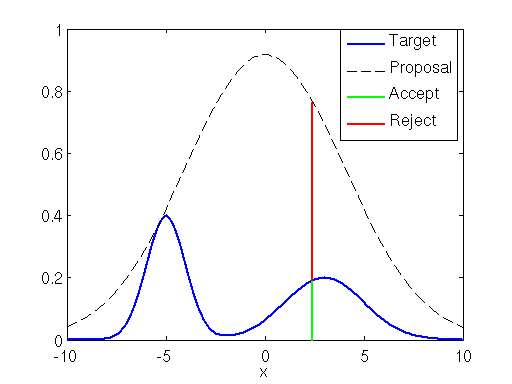
\includegraphics[width=0.5\linewidth]{figs/rejection.png}
			\caption{Rejection sampling visualized with $\widetilde{p}(z)$ in blue and $kq(z)$ in black.
				Source: \url{https://theclevermachine.files.wordpress.com}}
			\label{fig:rejection}
		\end{figure}
		
		\emph{Adaptive rejection sampling} constructs the proposal function on the fly (typically piecewise linear in $\ln p(z)$).
		Sampled point which are not accepted are used to refine the proposal function.
		
	\end{easylist}
		\begin{easylist}[itemize]
			\ListProperties(Space=\listSpace, Space*=\listSpace)
	# \emph{Importance sampling} computes expectations without sampling from $\widetilde{p}(z)$.
	A proposal function $\widetilde{q}(z)$ is used, and the success depends crucially on how close $\widetilde{q}(z)$ is to $\widetilde{p}(z)$.
	\begin{equation*}
		\E [f] = \int f(\vect{z}) p(\vect{z}) \, d \vect{z}
		\simeq \frac{1}{L} \sum_{\ell = 1}^{L} \frac{p(\vect{z}^\ell)}{q(\vect{z}^\ell)} f(\vect{z}^\ell)
		= \frac{1}{L} \sum_{\ell = 1}^{L} w_\ell f(\vect{z}^\ell)
	\end{equation*}
	The weights $w_\ell$ measure how close the distributions are.
	In general the distributions need not be normalized.
	
	# \emph{Sampling importance-resampling} uses a samling distribution $q(\vect{z})$, but unlike in rejection sampling we need not find a constant $k$.
	First $L$ samples are drawn from $q(\vect{z})$, then for each $\vect{z}^\ell$ a weight $w_\ell = p(\vect{z})/q(\vect{z})$ is assigned.
	New samples are then drawn (bootstrapped) from the distribution given by the samples $\vect{z}^1, \ldots, \vect{z}^\ell$ and corresponding weights $w_1, \ldots, w_\ell$.
\end{easylist}

\subsection*{Markov Chain Monte Carlo}
\begin{easylist}[itemize]
	\ListProperties(Space=\listSpace, Space*=\listSpace)
	# TODO
\end{easylist}

% ----------------------------------------------------------------------------
\subsection{Continuous Latent Variables}
\begin{easylist}[itemize]
	\ListProperties(Space=\listSpace, Space*=\listSpace, Numbers1=l, FinalMark1={)})
	# sdf
\end{easylist}

% ----------------------------------------------------------------------------
\subsection{Sequential Data}
\begin{easylist}[itemize]
	\ListProperties(Space=\listSpace, Space*=\listSpace, Numbers1=l, FinalMark1={)})
	# sdf
\end{easylist}

% ----------------------------------------------------------------------------
\subsection{Combining Models}
\begin{easylist}[itemize]
	\ListProperties(Space=\listSpace, Space*=\listSpace, Numbers1=l, FinalMark1={)})
	# sdf
\end{easylist}

% ----------------------------------------------------------------------------
















\clearpage
\section{Exercises}

% ----------------------------------------------------------------------------
\subsection{Introduction}
\subsubsection*{Exercise 1.2}
We start with Equation (1.4) from the book and differentiate it with respect to $w_i$:
\begin{align*}
	\partial_{w_i} \tilde{E}(\vect{w})
	&= \sum_{n=1}^{N} \left[ y(x_n, \vect{w}) - t_n \right] \partial_{w_i} y(x_n, \vect{w}) + \lambda w_i \\
	&= \sum_{n=1}^{N} \left[ y(x_n, \vect{w}) - t_n \right] (x_n)^i + \lambda w_i \\
	&= \sum_{n=1}^{N} \left[ \sum_{j=0}^{M} w_j (x_n)^j - t_n \right] (x_n)^i + \lambda w_i = 0
\end{align*}
Multiplying through the factor $(x_n)^i$ and rearranging the terms yields
\begin{equation*}
	\sum_{j=0}^{M} w_j \underbrace{\sum_{n=1}^{N} (x_n)^{i+j}}_{A_{ij}}
	+
	\lambda w_i = \underbrace{\sum_{n=1}^{N}  (x_n)^i t_n}_{T_{ij}},
\end{equation*}
where the definitions of $A_{ij}$ and $T_{ij}$ are identical to those given in Exercise 1.1.
Finally we employ the Kronecker delta symbol $\delta_{ij}$ to pull the $w_i$ into the sum, since $\lambda w_i = \sum_{j=0}^{M} \lambda \delta_{ij} w_j$ we have
\begin{equation*}
	\sum_{j=0}^{M}  \left( A_{ij} + \delta_{ij} \lambda \right) w_j
	 = T_{ij}.
\end{equation*}
This solves the problem.
Notice that in vector notation this system can be written as 
\begin{equation*}
	\left( \vect{\Phi}^T \vect{\Phi} + \vect{I}\lambda \right) \vect{w} = \vect{\Phi}^T \vect{t},
\end{equation*}
where $\vect{\Phi}_{ij}= (x_i)^j$.
Solving the system solves the regularized polynomial fitting problem.


\subsubsection*{Exercise 1.8}
We first show that $\E \left[x\right] = \mu$.
We define $K(\sigma) = 1 / \sqrt{2 \pi} \sigma$ and evaluate the integral
\begin{align*}
	\E \left[x\right] &= \int K(\sigma) \exp \left( - \frac{1}{2 \sigma^2} \left(x - \mu \right)^2 \right) x \, dx \\
	&= \int K(\sigma) \exp \left( - \frac{1}{2 \sigma^2} z^2 \right) (z + \mu) \, dz \tag{change of variables}\\
	&= \int K(\sigma) \exp \left( - \frac{1}{2 \sigma^2} z^2 \right) z \, dz 
	+
	 \mu \int K(\sigma) \exp \left( - \frac{1}{2 \sigma^2} z^2 \right) \, dz \\
	 & = 0 + \mu,
\end{align*}
where the first integral in the second to last line is zero because it's an odd function integrated over the real line, and the second integral evaluates to $\mu$ since the integrand is unity (it's a centered normal distribution, which has integral $1$).

The second part of the problem asks us to verify that $\E \left[ x^2 \right] = \mu^2 + \sigma^2$.
We factor the normal distribution as $\N\left( x \mid \mu, \sigma^2\right) = K(\sigma^2) E(\sigma^2)$, where
\begin{alignat*}{3}
	& K(\sigma^2) = \left( 2 \pi \sigma^2 \right)^{-1/2} 
	&& \qquad \frac{\partial K}{\partial \sigma^2} = - \left( 2 \pi \sigma^2 \right)^{-3/2} \pi = -K(\sigma^2)^3 \pi \\
	& E(\sigma^2) = \exp \left( - \frac{1}{2 \sigma^2} \left( x - \mu \right)^2 \right)
	&& \qquad \frac{\partial E}{\partial \sigma^2} = \frac{1}{2\sigma^4} \left( x - \mu\right)^2 E(\sigma^2).
\end{alignat*}
We expedite notation by writing these functions as $K$ and $E$, and their derivatives with respect to $\sigma^2$ as $K'$ and $E'$.
Using the product rule of calculus, we have
\begin{gather*}
	\frac{\partial}{\partial \sigma^2} \left( \int K(\sigma^2) E(\sigma^2) \, dx = 1 \right) \\
	\int K' E + K E' \, dx = 0 \\
	\int KE \left( -\pi K^2 + \frac{1}{2 \sigma^4} (x - \mu)^2 \right) \, dx = 0.
\end{gather*}
Substituting $- \pi K^2 = - 1 / (2 \sigma^2)$, expanding the square term, multiplying out the $KE$ term and performing the integrals, we obtain
\begin{equation*}
	-\frac{1}{2\sigma^2} + \frac{1}{2 \sigma^4} \int KE x^2 \, dx + 0 - \frac{\mu^2}{2 \sigma^4} = 0,
\end{equation*}
and solving this for the unknown integral yields $\operatorname{E}\left[x^2\right] = \int KE x^2 \, dx = \mu^2 + \sigma^2$
as required.

To show that Equation (1.51) from the book holds, notice that
\begin{align*}
	\var \left[ x \right] &= \E\left[ (x - \E\left[x\right])^2\right] 
	= \E\left[ x^2 - 2 x \mu + \mu ^2\right] \\
	&= \E\left[ x^2\right] - 2 \mu^2 + \mu^2 
	= \E\left[ x^2\right] - \E\left[ x\right]^2,
\end{align*}
where we have used $\mu$ interchangeably with $\E\left[ x\right]$. 



\subsubsection*{Exercise 1.10}
Recall that the definition of the expected value is
$\E\left[x\right] = \int p(x) x \, dx$, and that $\int p(x) \, dx = 1$
Statistical independence means that $p(x, y)$ factors as $p(x)p(y)$, so we have
\begin{align*}
	\E\left[x + y\right] &= \iint p(x, y) (x+y) \, dx \, dy 
	= \iint p(x) p(y) (x+y) \, dx \, dy \tag{independence} \\
	&= \iint p(x) p(y) x \, dx \, dy + \iint p(x) p(y) y \, dx \, dy \\
	&= \int p(y) \left( \int  p(x)  x \, dx \right) \, dy + \int p(y) y \left( \int p(x)  \, dx \right) \, dy \\
	&= \int p(y) \left( \E \left[ x \right] \right) \, dy + \int p(y) y \, dy \tag{by definition} 
	= \E\left[x\right] + \E\left[y\right]
\end{align*}

To show that $\var\left[x + y\right] = \var\left[x\right] + \var\left[y\right]$, we use the preceding result along with the definition from Equation (1.38) in \cite{bishop_pattern_2011}  $\var\left[x\right] = \E\left[ (x - \E\left[x\right])^2\right]$ to write
\begin{align*}
	\var\left[x + y\right] &= \E\left[ \left( (x + y) - \E \left[ x + y \right] \right)^2\right] \\
	&= \E\left[ \left( \left(x - \E\left[x\right]\right) + \left(y - \E\left[y\right]\right) \right)^2\right] \tag{rearranging} \\
	&= \E\left[  \left(x - \E\left[x\right]\right)^2 + 2 \left(x - \E\left[x\right]\right) \left(y - \E\left[y\right]\right) + \left(y - \E\left[y\right]\right)^2\right] \\
	&= \E\left[  \left(x - \E\left[x\right]\right)^2 \right]
	+
	\underbrace{\E\left[   2 \left(x - \E\left[x\right]\right) \left(y - \E\left[y\right]\right) \right]}_{0}
	+
	\E\left[   \left(y - \E\left[y\right]\right)^2\right] \\
	&= \var\left[x\right] + \var\left[y\right].
\end{align*}
The cross term vanishes since $x$ and $y$ are independent.
We will not show this in detail, but it can be shown by first noticing that $\E \left[xy\right] = \E \left[x\right] \E \left[y\right]$ when $x$ and $y$ are independent, and then showing that $\E\left[    \left(x - \E\left[x\right]\right) \right] = \E\left[ x \right] - \E\left[ x \right] = 0$.

\subsubsection*{Exercise 1.15}
Due to the size of this problem, we split the solution into parts.
\begin{easylist}[enumerate]
	\ListProperties(Space=\listSpace, Space*=\listSpace, Numbers1=l, FinalMark1={)})
	# The redundancy is present due to the fact fact multiplication is commutative, so the weights may be factored out.
	For instance, when $M=2$, we see that 
	\begin{equation*}
		w_{ij}x_i x_j + w_{ji} x_j x_i = (w_{ij} + w_{ji}) x_i x_j = \widetilde{w}_{ij} x_i x_j.
	\end{equation*}
	We remove redundancy by ordering the products in a common term with $i_1 \geq i_2 \geq \cdots \geq i_M$.
	This ordering corresponds to Equation (1.134).
	
	For instance, instead of summing over terms with $x_1 x_2 x_3$, $x_1 x_3 x_2$, $x_2 x_1 x_3$ and so forth, we make use of a common weight for the $x_3 x_2 x_1$-term.
	
	# The total number of terms equals the number of terms in the nested sum
	\begin{equation*}
		n(D, M) = \sum_{i_1 = 1}^{D} 
		\sum_{i_2 = 1}^{i_1}
		\cdots
		\sum_{i_M = 1}^{i_{M - 1}} 1,
	\end{equation*}
	which contains $M$ sums.
	To prove the recursive formula, we expand the outer sum and notice that the result is $D$ nested sums over $M-1$ sums each.
	We have
	\begin{align*}
		n(D, M) &= \sum_{i_1 = 1}^{D} 
		\sum_{i_2 = 1}^{i_1}
		\cdots
		\sum_{i_M = 1}^{i_{M - 1}} 1 \\
		&= 
		\left( 
		\sum_{i_2 = 1}^{1}
		\cdots
		\sum_{i_M = 1}^{i_{M - 1}} 1
		\right)+\left( 
		\sum_{i_2 = 1}^{2}
		\cdots
		\sum_{i_M = 1}^{i_{M - 1}} 1
		\right)+
		\cdots
		+\left( 
		\sum_{i_2 = 1}^{D}
		\cdots
		\sum_{i_M = 1}^{i_{M - 1}} 1 \right) \\
		&= n(D=1, M-1) + n(D=2, M-1) + \cdots + n(D=D, M-1) \\
		&= \sum_{i=1}^{D} n(i, M-1).
	\end{align*}
	
	# We skip the base case, which is easily verified.
	Assuming the result holds for $D$, we we show that it holds for $D+1$ by writing
	\begin{align*}
		\sum_{i=1}^{D + 1} \frac{(i +M - 2)!}{(i-1)!\, (M-1)!} &=
		\sum_{i=1}^{D} \frac{(i +M - 2)!}{(i-1)! \, (M-1)!}
		+  \frac{(D+M-1)!}{D! \, (M-1)!}.
	\end{align*}
	The sum on the right hand side is the given result for $D$, which we assume is true.
	Substituting this fact, we write
	\begin{align*}
		\sum_{i=1}^{D + 1} \frac{(i +M - 2)!}{(i-1)! \, (M-1)!} &=
		\frac{(D + M - 1)!}{(D- 1)! \, M!}
		+  \frac{(D+M-1)!}{D! \, (M-1)!} \\
		&=
		\frac{(D + M - 1)! \, D}{D! \, M!}
		+  \frac{(D+M-1)! \, M}{D! \, M!} \\
		&=
		\frac{(D + M - 1)! \, (D + M)}{D! \, M!} = \frac{(D + M)!}{D!\, M!} \\
		&=\frac{((D+1) + M - 1)!}{((D+1) - 1)! \, M!},
	\end{align*}
	which shows that the result holds for $D+1$ when it holds for $D$.
	
	# We skip the base case of the inductive argument, as it should be easy to carry out.
	
	The inductive step is performed as follows.
	Below, the first equality comes from Equation (1.135) in the book,
	the second comes from assuming the result holds for $M-1$,
	and the third comes from Equation (1.136).
	\begin{equation*}
		n(D, M) = \sum_{i=1}^{D} n(i, M - 1)
		= \sum_{i=1}^{D} \frac{(i +M - 2)!}{(i-1)!\, (M-1)!} 
		= 
		 \frac{(D + M - 1)!}{(D - 1)! \, M !}.
	\end{equation*}
	Comparing the first and final expression, we observe that if we assume the relation holds for $M-1$, it does indeed hold for $M$ too.
\end{easylist}


\subsubsection*{Exercise 1.21}
Starting with the inequality $a \leq b$, we multiply both sides by $a > 0$ to obtain $a^2 \leq ab$.
We can take the square root of both sides and preserve the inequality, since the square root is monotonically increasing.
Doing so, we obtain the desired inequality.

To prove the integral inequality, we apply the inequality on each term in Equation (1.78), then replace the integral over $\mathcal{R}_1 \cup \mathcal{R}_2$ with the real line:
\begin{align*}
	p(\text{mistake}) &= \int_{\mathcal{R}_1} p(\vect{x}, \mathcal{C}_2) \, d 
	\vect{x}
	+
	\int_{\mathcal{R}_2} p(\vect{x}, \mathcal{C}_1) \, d \vect{x} \\
	&\leq 
	 \int_{\mathcal{R}_1} \left\{ p(\vect{x}, \mathcal{C}_1) \, p(\vect{x}, \mathcal{C}_2) \right\}^{1/2} \, d \vect{x}
	+
	\int_{\mathcal{R}_2} \left\{ p(\vect{x}, \mathcal{C}_2) 
	\, p(\vect{x}, \mathcal{C}_1) \right\}^{1/2} \, d \vect{x} \\
	&= \int \left\{ p(\vect{x}, \mathcal{C}_2) \, p(\vect{x}, \mathcal{C}_1) \right\}^{1/2} \, d \vect{x}
\end{align*}

\subsubsection*{Exercise 1.25}
This closely follows the derivation in Section 1.5.5.
If $\vect{x} \in \R^n$ and $\vect{t} \in \R^m$, we view
$\E \left[L (\vect{t}, \vect{y} (\vect{x}))\right]$ as a functional from the set of functions $\{ f \mid f: \R^n \to \R^m \}$ to $\R$.
Comparing the ordinary derivative and the functional derivative, we see that
\begin{align*}
	f(\vect{x} + \vect{\epsilon}) &= f(\vect{x}) 
	+
	\vect{\epsilon}^T \nabla f(\vect{x}), \quad \text{and}
	\\
	F(\vect{y}(\vect{x}) + \epsilon \vect{\eta}(\vect{x})) &=
	F(\vect{y}(\vect{x})) + \epsilon \int \int  \vect{\eta}^T
	\delta_{\vect{y}_j(\vect{x})} F(\vect{y}(\vect{x}))
	  \, d \vect{t} \, d\vect{x} \\
	&=
	 F(\vect{y}(\vect{x}))
	+
	\epsilon \sum_{j=1}^{n}
	 \int \underbrace{\left( \int \frac{\delta F(\vect{y}(\vect{x}))}{\delta \vect{y}_j(\vect{x})} \, d \vect{t} \right)}_{\text{must be } 0} \eta_j (\vect{x}) \, d \vect{x}.
\end{align*}
The above condition implies that
\begin{equation*}
	\left( \int \frac{\delta F(\vect{y}(\vect{x}))}{\delta \vect{y}_j(\vect{x})} \, d \vect{t} \right)=
	2 \int ( \vect{y}_j(\vect{x}) - \vect{t}_j) p (\vect{x}, \vect{t}) \, d\vect{t}
	= 0,
\end{equation*}
which, following the derivation leading to Equation (1.89), leads to
\begin{equation*}
	\vect{y}_j(\vect{x}) = \int t_j p (\vect{t} \mid \vect{x}) \, d \vect{t} = \E_{\vect{t}} \left[ t_j \mid \vect{x} \right].
\end{equation*}
This applies to any  component $j$ of $\vect{y}(\vect{x})$, so $\vect{y}(\vect{x}) = \E_{\vect{t}} \left[ \vect{t} \mid \vect{x} \right]$.
To show that this reduces to Equation (1.89) in the case of a single target variable, simply define $\vect{t} := (t)$, i.e. a vector with one component.




\subsubsection*{Exercise 1.33}
A hint as to why this is true is given on page 54, which states that $\H\left[y 
\mid x\right]$ is ``the average additional information needed to specify $y$, 
given $x$.''
If the conditional entropy is zero, then $y$ must be completely specified by $x$, i.e. a function of $x$.
If $\H\left[y \mid x\right] = 0$, then
\begin{equation*}
	\sum_i \sum_j p(x_i, y_j) \ln p (y_j \mid x_i) = 0.
\end{equation*}
Using $ p(x_i, y_j) = p(y_j \mid x_i) p(x_i)$ and rearranging the sums, we obtain
\begin{equation*}
	\sum_i p(x_i) \left[ \sum_j p(y_j \mid x_i)  \ln p (y_j \mid x_i) \right] = 0.
\end{equation*}
We know that $0 \leq p (x_i) \leq 1$ for every $x_i$.
Assuming now that $p (x_i) > 0$, the bracketed term must be zero for every $i$, i.e.
\begin{equation*}
	\sum_j p(y_j \mid x_i)  \ln p (y_j \mid x_i) = 0 \quad \text{for every } i.
\end{equation*}
Consider now the term $p(y_j \mid x_i)  \ln p (y_j \mid x_i)$.
The functional form of this term is $z \ln z$, and this function is negative 
except when $z = 0$ and when $z=1$, where it is zero.
Since we are adding terms that are either negative or zero, and the sum must 
evaluate to zero, every term in the sum must be zero.
Therefore, $p(y_j \mid x_i)$ must be 0 or 1 for each value of $y_j$.
However, since $\sum_j p(y_j \mid x_i) = 1$, every value of $p(y_j \mid x_i)$ 
must be zero except for one.
In other words, $x_i$ completely determines $y_j$.


\subsubsection*{Exercise 1.38}
We wish to prove Equation (1.115) based on Equation (1.114).
Clearly the case $M=1$ is true, and we assume the case $M=2$ is true, since this is given by Equation (1.114).
For the inductive step, we assume the identity holds in the base case, and in 
the $M-1$ case, and then
\begin{align*}
	f \left( \sum_{i=1}^{M} \lambda_i x_i \right)
	&= f \left( \sum_{i=1}^{M-1} \lambda_i x_i + \lambda_M x_M \right)
	= f \left( \frac{\sum_{k=1}^{M-1} \lambda_k}{\sum_{k=1}^{M-1} \lambda_k} \sum_{i=1}^{M-1} \lambda_i x_i + \lambda_M x_M \right).
\end{align*}
The sum of $\sum_{k=1}^{M-1} \lambda_k$ and $\lambda_M$ is unity, and $\sum_{i=1}^{M-1} \lambda_i x_i / \sum_{k=1}^{M-1} \lambda_k$ is a weighted average of $x$-values.
Since it's a weighted average, it may be treated as just another $x$-value.

Applying the base case for two $x$ values, we obtain
\begin{equation*}
	f \left( \frac{\sum_{k=1}^{M-1} \lambda_k}{\sum_{k=1}^{M-1} \lambda_k} \sum_{i=1}^{M-1} \lambda_i x_i + \lambda_M x_M \right)
	\leq
	\left( \sum_{k=1}^{M-1} \lambda_k \right) f \left( 
	\frac{1}{\sum_{k=1}^{M-1} \lambda_k} \sum_{i=1}^{M-1} \lambda_i x_i
	 \right)
	+
	\lambda_M f \left( x_M \right).
\end{equation*}
Now we can appeal to the $M-1$ case of the inequality, which we assume to be true by the induction hypothesis.
We can appeal to it since the $\lambda_i / \sum_{k=1}^{M-1} \lambda_k$ are normalized and sum to unity in the equation above due to the normalizing factor in front of the sum.
To ease notation, we define $\alpha = \sum_{k=1}^{M-1} \lambda_k$ and write
\begin{equation*}
\alpha f \left( 
 \sum_{i=1}^{M-1} \frac{\lambda_i}{\alpha} x_i
\right)
+
\lambda_M f \left( x_M \right)
\leq
\alpha \left( \sum_{i=1}^{M-1} \frac{\lambda_i}{\alpha} f(x_i) \right)
+
\lambda_M f \left( x_M \right)
=
\sum_{i=1}^{M} \lambda_i f(x_i).
\end{equation*}
This proves the Jensen inequality.


% ----------------------------------------------------------------------------
\subsection{Probability Distributions}
\subsubsection*{Exercise 2.6}
We split this problem into three parts: (a) expected value, (b) variance and (c) mode.
\begin{easylist}[enumerate]
	\ListProperties(Space=\listSpace, Space*=\listSpace, Numbers1=l, FinalMark1={)})
	# The \textbf{expected value} is computed from the definition as
	\begin{align*}
		\E[\mu] &= \int \mu p(\mu) \, d\mu =  \frac{\Gamma(a + b)}{\Gamma(a ) \Gamma( b)} \int_0^1 \mu \, \mu^{a-1} (1- \mu)^{b-1} \, d\mu \\
		&= \frac{\Gamma(a + b)}{\Gamma(a ) \Gamma( b)} \int_0^1  \mu^{(a+1)-1} (1- \mu)^{b-1} \, d\mu \tag{re-cast as Beta} \\ 
		&= \frac{\Gamma(a + b)}{\Gamma(a ) \Gamma( b)} \frac{\Gamma(a +1 ) \Gamma( b)}{\Gamma(a + b + 1)} = \frac{a}{a + b},
	\end{align*}
	where we used Equation (2.265) from \cite{bishop_pattern_2011}, along with $\Gamma(x+1) = x\Gamma(x)$.
	
	# To compute the \textbf{variance}, we will employ $\var[\mu] = \E[\mu^2] - \E[\mu]^2$.
	Similarly to the sub-problem above, we observe that
	\begin{align*}
	\E[\mu^2] &= \frac{\Gamma(a + b)}{\Gamma(a ) \Gamma( b)} \int_0^1  \mu^{(a+2)-1} (1- \mu)^{b-1} \, d\mu \\
	&= \frac{\Gamma(a + b)}{\Gamma(a ) \Gamma( b)} \frac{\Gamma(a +2 ) \Gamma( b)}{\Gamma(a + b + 2)}
	= \frac{(a+1) a}{(a + b +1) (a+b)},
	\end{align*}
	where in the last equality we have used $\Gamma(x+2) = (x+1)x \Gamma(x)$, which is simply repeated application of $\Gamma(x+1) = x\Gamma(x)$ twice.
	
	The remaining computation is
	\begin{equation*}
		\var[\mu] = \E[\mu^2] - \E[\mu]^2 = \frac{(a+1) a}{(a + b +1) (a+b)} - \left( \frac{a}{a + b} \right),
	\end{equation*}
	which after some manipulation equals the desired result.
	We omit the details.
	
	# The \textbf{mode} is the maximum of the distribution.
	We differentiate the p.d.f. using the product rule of calculus to obtain
	\begin{equation*}
		p'(\mu) = (a-1) \mu{a-2} (1-\mu)^{b-1}
		+
		\mu^{a-1} (b-1) (1-\mu)^{b-2}(-1) = 0.
	\end{equation*}
	Diving by $\mu^a$ and $(1-\mu)^b$ and rearranging, we obtain
	\begin{equation*}
		\frac{(a-1)}{(b-1)} \frac{(1 - \mu)}{\mu} = 1.
	\end{equation*}
	Solving the equation above for $\mu$ yields  $(a-1) / (a + b - 2)$ as required.
\end{easylist}

\subsubsection*{Exercise 2.8}
The \textbf{first part} is to prove Equation (2.270). 
We apply the definitions of $E_x \left[ x \mid y \right]$ and $E_y [f(y)]$ in turn, and then the product rule of probability.
Doing so, we observe that
\begin{align*}
	E_y \left[ E_x \left[ x \mid y \right]  \right] &= 
	E_y \left[ \int x p (x \mid y) \, dx  \right] 
	= \int \left( \int x p (x \mid y) \, dx \right)  p(y) \, dy \\
	&=  \iint x p(x, y) \, dx \, dy = \E[x].
\end{align*}

The \textbf{second part}, which consists of proving Equation (2.271), is slightly more involved.
It helps to keep track of whether the quantities are constants, functions of $x$ or functions of $y$.
It's also useful to know, from the definition of conditional variance, that
\begin{equation}
\label{eqn:conditional_variance}
	\var_x[ x \mid y ] 
	=
	\int p(x \mid y) \left( x - E_x \left[ x \mid y \right] \right)^2 \, dx
	=
	 \E_x [x^2 \mid y] - \E_x [x \mid y]^2.
\end{equation}
The result above does not come as a surprise, since it's merely the familiar result for variance, i.e. $\var_x[ x ] = \E_x [x^2] - \E_x [x ]^2$, conditioned on $y$ in every term.

Let's examine the \textbf{first term} in the right hand side of (2.270) first, i.e. $\E_y \left[ \var_x[ x \mid y ]  \right]$.
Using Equation \eqref{eqn:conditional_variance} above, we see that
\begin{align}
	\nonumber \E_y \left[ \var_x[ x \mid y ]  \right] &=  \E_y \left[ \E_x [x^2 \mid y] - \E_x [x \mid y]^2  \right]
	=
	\E_y \left[ \E_x [x^2 \mid y] \right] - \E_y \left[ \E_x [x \mid y]^2  \right] \\
	\label{eqn:ch2_prob8a} &= \E[x^2] - \E_y \left[ \E_x [x \mid y]^2  \right],
\end{align}
where we used Equation (2.270) from the book in the last equality.

We now investigate the \textbf{second term} in Eqn (2.270), i.e. 
$\var_y \left[ \E_x \left[ x \mid y \right] \right]$.
Using the definition of variance (Equation (1.38) in \cite{bishop_pattern_2011}), followed by Equation (2.270) from the book, and the linearity of the expected value, we obtain
\begin{align}
\nonumber \var_y \left[ \E_x \left[ x \mid y \right] \right]
&= \E_y \left[ 
\left( \underbrace{\E_x \left[ x \mid y \right]}_{f(y)} - 
\underbrace{\E_y \left[ \E_x \left[ x \mid y \right] \right]}_{\text{scalar}} 
\right)^2 \right]   \\
\nonumber &= \E_y \left[ 
\left( \E_x \left[ x \mid y \right] - 
\E[x]
\right)^2 \right] \tag{previous result} \\
\nonumber &= \E_y \left[ 
\E_x \left[ x \mid y \right]^2
-2 \E_x \left[ x \mid y \right] \E[x]
+\E[x]^2
\right] \tag{multiply} \\
\nonumber &= \E_y \left[ 
\E_x \left[ x \mid y \right]^2 \right]
-\E_y \left[ 2 \E_x \left[ x \mid y \right] \E[x] \right]
+\E_y \left[ \E[x]^2
\right] \tag{linearity} \\
 \nonumber &= \E_y \left[ 
\E_x \left[ x \mid y \right]^2 \right]
- 2 \E_y \left[ \E_x \left[ x \mid y \right] \right] \E[x] 
+ \E[x]^2
 \tag{constants}\\
\label{eqn:ch2_prob8b} &= \E_y \left[ 
 \E_x \left[ x \mid y \right]^2 \right]
 - \E[x]^2
\end{align}
Finally, adding Equations \eqref{eqn:ch2_prob8a} and \eqref{eqn:ch2_prob8b} produces the result we're after.


\subsubsection*{Exercise 2.15}
The entropy is given by $\H[p(\vect{x})] = - \int p(\vect{x}) \ln p(\vect{x}) \, d\vect{x}$ from it's definition, and we start by computing the logarithm of $p(\vect{x})$, which is
\begin{equation*}
	\ln p(\vect{x}) = -\frac{D}{2} \ln (2 \pi ) - \frac{1}{2} \ln \abs{\vect{\Sigma}} - \frac{1}{2} (\vect{x} - \vect{\mu})^T \vect{\Sigma}^{-1}(\vect{x} - \vect{\mu}).
\end{equation*}
Defining $\Delta^2$ as $(\vect{x} - \vect{\mu})^T \vect{\Sigma}^{-1}(\vect{x} - \vect{\mu})$ (see Equation (2.44) in the book), we have
\begin{equation*}
	\H[p(\vect{x})] = - \int p(\vect{x}) \ln p(\vect{x}) \, d\vect{x} = 
	\frac{D}{2} \ln (2 \pi ) + \frac{1}{2} \ln \abs{\vect{\Sigma}}
	+ \frac{1}{2}\int   p(\vect{x}) \Delta^2 \, d\vect{x},
\end{equation*}
since $\int K p(\vect{x}) \, d\vect{x} = K$ for constants $K$ such as $D \ln (2\pi) /2$.
The only troublesome term is the last one, so what remains to do is show that $\int p(\vect{x}) \Delta^2 \, d\vect{x} = D$.
If we can show this, then we've proven the equation given in the problem statement.

We will now show that $\int p(\vect{x}) \Delta^2 \, d\vect{x} = D$.
First, however, we'll present a result for the univariate Gaussian, which we will need later on. 
Here's the univariate result, easily verified by means of partial integration.
\begin{equation}
\label{eqn:ch2_problem15_a}
	\frac{1}{\sqrt{2 \pi} \sigma} \int \exp \left( - \frac{x^2}{2 \sigma^2}\right) \, dx = 
	\frac{1}{\sqrt{2 \pi} \sigma} \int \frac{x^2}{\sigma^2} \exp \left( - \frac{x^2}{2 \sigma^2}\right) \, dx = 1
\end{equation}

We now rotate into $\vect{y}$-space by $\vect{y} = \vect{U}(\vect{x} - \vect{\mu})$, which diagonalizes $\vect{\Sigma}^{-1}$.
From Equations (2.50) and (2.56) in \cite{bishop_pattern_2011}, we see that the integral $\int \Delta^2  p(\vect{x}) \, d\vect{x}$ now becomes
\begin{align*}
	\int_{\R^D} \left( \sum_{i=1}^{D} \frac{y_i^2}{\lambda_i} \right)
	\prod_{j=1}^{D} \frac{1}{(2 \pi \lambda_j)^{1/2}} 
	\exp \left( - \frac{y_j^2}{2 \lambda_j} \right) \, d \vect{y}.
\end{align*}
Multiplying the product into the sum, and integrating each term, we have
\begin{align*}
\sum_{i=1}^{D} \int_{\R^D}  \frac{y_i^2}{\lambda_i} 
\prod_{j=1}^{D} \frac{1}{(2 \pi \lambda_j)^{1/2}} 
\exp \left( - \frac{y_j^2}{2 \lambda_j} \right)  \, d \vect{y},
\end{align*}
where $d \vect{y} := d y_1 \, d y_2 \, \cdots \, d y_D$.
To clarify the meaning of the equation above, let's focus on term $i$ in the outer sum and write out the products more explicitly, the above integral is
\begin{equation}
\label{eqn:ch2_problem15_b}
	\left( \int \frac{1}{(2 \pi \lambda_1)^{1/2}} \exp \left( - \frac{y_1^2}{2 \lambda_1} \right) \, d y_1 \right)
	\cdots
	%\left( \int \frac{1}{(2 \pi \lambda_j)^{1/2}} \exp \left( - \frac{y_j^2}{2 \lambda_1} \right) \, d y_j \right)
	\left( \int \frac{1}{(2 \pi \lambda_D)^{1/2}} \exp \left( - \frac{y_D^2}{2 \lambda_D} \right) \, d y_D \right),
\end{equation}
but the $i$th factor is special, since it has the additional $y_i^2 / \lambda_i$ factor, i.e. it's given by
\begin{equation}
\label{eqn:ch2_problem15_c}
	\left( \int \frac{1}{(2 \pi \lambda_i)^{1/2}} \frac{y_i^2}{\lambda_i}   \exp \left( - \frac{y_i^2}{2 \lambda_i} \right) \, d y_i \right).
\end{equation}
Now comes the crucial observation; every factor in \eqref{eqn:ch2_problem15_b} except the $i$th is a univariate Gaussian, so these integrals evaluate to 1.
The special $i$th term \eqref{eqn:ch2_problem15_c} is in same functional form as Equation \eqref{eqn:ch2_problem15_a} (with $\lambda_i = \sigma^2$), so it also evaluates to 1.
Therefore the product of integrals for every term $i$ evaluates to a product of ones, and the sum is simply
\begin{align*}
\sum_{i=1}^{D} \int_{\R^D}  \frac{y_i^2}{\lambda_i} 
\prod_{j=1}^{D} \frac{1}{(2 \pi \lambda_j)^{1/2}} 
\exp \left( - \frac{y_j^2}{2 \lambda_j} \right)  \, d \vect{y}
=
\sum_{i=1}^{D} 1 = D.
\end{align*}
We've shown that $\int p(\vect{x}) \Delta^2 \, d\vect{x} = D$, and this solves the problem.

\subsubsection*{Exercise 2.20}
We expand $\vect{a}$ in the eigenvector basis of $\vect{\Sigma}$, writing $\vect{a} = \sum_i \alpha_i \vect{u}_i$.
Using the fact that $\vect{u}_i \vect{u}_j = \delta_{ij}$, we have
\begin{align*}
	\vect{a}^T \vect{\Sigma} \vect{a} 
	&= \vect{a}^T \vect{\Sigma} \sum_i \alpha_i \vect{u}_i
	= \vect{a}^T \sum_i \alpha_i \vect{\Sigma} \vect{u}_i
	= \vect{a}^T \sum_i \alpha_i \lambda_i \vect{u}_i \\
	&= \sum_j \alpha_j \vect{u}^T_j \sum_i \alpha_i \lambda_i \vect{u}_i
	= \sum_i \alpha_i^2 \lambda_i.
\end{align*}
If $\lambda_i > 0$ for every $i$, then clearly the sum is positive---so it's sufficient.
On the other hand, if the sum is positive, then no $\lambda_i$ can be negative or zero.
If it were, we could choose $\vect{a}$ in the direction of the corresponding eigenvector and obtain a negative sum, which would be a contradiction.
In other words, it's a also necessary condition that $\lambda_i > 0$ for every $i$.


\subsubsection*{Exercise 2.27}
We split this exercise into two parts.
\begin{easylist}[enumerate]
	\ListProperties(Space=\listSpace, Space*=\listSpace, Numbers1=l, FinalMark1={)})
	# We wish to show that $\E[\vect{x} + \vect{z}] = \E[\vect{x}] + \E[ \vect{z}]$.
	 Using the definition of the expected value, along with independence, we see that
	\begin{align*}
		\E[\vect{x} + \vect{z}] &= \iint (\vect{x} + \vect{z}) p(\vect{x}, \vect{z}) \, d\vect{x} \, d\vect{z} 
		= \iint (\vect{x} + \vect{z}) p(\vect{x}) p(\vect{z}) \, d\vect{x} \, d\vect{z}\\
		&= \int \vect{x} p(\vect{x}) p(\vect{z}) \, d\vect{x} \, d\vect{z} + \int \vect{z} p(\vect{x}) p(\vect{z}) \, d\vect{x} \, d\vect{z}
		= \E[\vect{x}] + \E[ \vect{z}].
	\end{align*}
	
	# As in the previous sub-problem, we use the definition to obtain
	\begin{align*}
	\cov[\vect{x} + \vect{z}] &= \E \left[ (\vect{x} + \vect{z} - \E[\vect{x} + \vect{z}]) (\vect{x} + \vect{z} - \E[\vect{x} + \vect{z}])^T \right] \\
	&= \E \left[ (\vect{x} - \E[\vect{x}] + \vect{z} - \E[\vect{z}]) (\vect{x} - \E[\vect{x}] + \vect{z} - \E[\vect{z}])^T \right].
	\end{align*}
	We wish to expand the inner square term.
	In order to avoid too heavy notation, we introduce $\vect{a}:= \vect{x} - \E[\vect{x}]$ and $\vect{b} := \vect{z} - \E[\vect{z}]$.
	From there, we observe that
	\begin{align*}
	\E \left[ (\vect{a} + \vect{b}) (\vect{a} + \vect{b})^T \right] = \E \left[ \vect{a}\vect{a}^T + \vect{a}\vect{b}^T + \vect{b}\vect{a}^T + \vect{b}\vect{b}^T \right]
	=
	\E \left[ \vect{a}\vect{a}^T  \right] +
	2 \E \left[ \vect{a}\vect{b}^T  \right] +
	\E \left[  \vect{b}\vect{b}^T \right].
	\end{align*}
	Using the definitions of $\vect{a}$ and $\vect{b}$, we see that this is
	\begin{equation*}
		\cov[\vect{x}] + 2 \cov[\vect{x}, \vect{z}] + \cov[\vect{z}],
	\end{equation*}
	and since the variables are independent,  $\cov[\vect{x}, \vect{z}] = \vect{0}.$
	We have shown that 
	\begin{equation*}
		\cov[\vect{x} + \vect{z}] = \cov[\vect{x}] + \cov[\vect{z}].
	\end{equation*}
\end{easylist}

\subsubsection*{Exercise 2.31}
If $y = x + z$, then $p_y(y) = p_x(x) * p_z(z)$, where $*$ denotes the \emph{convolution} operator.
To see why this is true, draw an $x$-$z$ coordinate system and sketch a line $x + z = a$.
The probability that $y = x + z = a$ is $p_y(y=a) = \int p_x(a - t) p_z(a) \, dt$, since this integrates over all possible ways to obtain the sum $a$.

In this case, when have $\vect{y} = \vect{x} + \vect{z}$, so we evaluate
\begin{align*}
	p_y(\vect{y}) &= p_x(\vect{x}) * p_z(\vect{z}) = 
	\int p_x(\vect{y} - \vect{t}) p_z(\vect{y}) \, d \vect{t} \\
	&=
	\int 
	\underbrace{\N \left( \vect{y} \mid \vect{\mu}_{\vect{x}} + \vect{t} , \vect{\Sigma}_{\vect{x}} \right) }_{p(\vect{y} \mid \vect{t})}
	\underbrace{\N \left( \vect{y} \mid \vect{\mu}_{\vect{z}} , 
	\vect{\Sigma}_{\vect{z}} \right)}_{p(\vect{y})}
	 \, d \vect{t}.
\end{align*}
Matching terms with Equations (2.109) and (2.110) we see that
\begin{equation*}
	p_y(\vect{y}) = \N \left( \vect{y} \mid 
	\vect{\mu}_{\vect{z}} + \vect{\mu}_{\vect{x}}
	, \vect{\Sigma}_{\vect{z}} + \vect{\Sigma}_{\vect{x}} \right).
\end{equation*}


\subsubsection*{Exercise 2.40}
The posterior is proportional to the prior times the likelihood.
When the prior is Gaussian, we have
\begin{align*}
	p( \vect{\mu} \mid \vect{X} ) &\propto p(\vect{\mu}) p (\vect{X} \mid \vect{\mu}) 
	= \N \left( \vect{\mu} \mid \vect{\mu}_0, \vect{\Sigma}_0 \right)
	\prod_{n=1}^{N}
	\N \left( \vect{x} \mid \vect{\mu}, \vect{\Sigma} \right).
\end{align*}
Let us ignore normalization constants and only consider the product of the exponential functions, this approach yields the following exponential function (which is not a p.d.f.)
\begin{align}
	\nonumber p( \vect{\mu} \mid \vect{X} ) & \propto \N \left( \vect{\mu} \mid \vect{\mu}_N, \vect{\Sigma}_N \right) \\
	\label{eqn:ch2_prob40_a} &= \exp\left( - \frac{1}{2} \left( 
	(\vect{\mu} - \vect{\mu}_0)^T \vect{\Sigma}_0^{-1} (\vect{\mu} - \vect{\mu}_0)
	+
	\sum_{n=1}^{N} (\vect{x}_n - \vect{\mu})^T \vect{\Sigma}^{-1} (x_n - \vect{\mu})
	 \right) \right).
\end{align}
We will multiply out the quadratic forms in Equation \eqref{eqn:ch2_prob40_a} above, and compare it to
\begin{equation}
\label{eqn:ch2_prob40_b}
	(\vect{\mu} - \vect{\mu}_N)^T \vect{\Sigma}_N^{-1} (\vect{\mu} - \vect{\mu}_N)
	= \vect{\mu}^T \vect{\Sigma}_N^{-1} \vect{\mu} - 2 \vect{\mu}_N^T \vect{\Sigma}_N^{-1} \vect{\mu} + \text{const}.
\end{equation}
Multiplying out the terms in the inner parenthesis of Equation \eqref{eqn:ch2_prob40_a} and rearranging, we obtain the following quadratic dependence on $\vect{\mu}$:
\begin{align*}
	\vect{\mu}^T \left( \vect{\Sigma}_0^{-1} + N \vect{\Sigma}^{-1} \right) \vect{\mu} - 2 
	\left( \vect{\mu}_0^T \vect{\Sigma}_0^{-1} + N \vect{\mu}_{\text{ML}}^T  \vect{\Sigma}^{-1} \right) \vect{\mu} + \text{const}.
\end{align*}
Comparing the above with Equation \eqref{eqn:ch2_prob40_b}, we immediately see that
\begin{align}
\label{eqn:ch2_prob40_c}
	\vect{\Sigma}_N^{-1} &= \vect{\Sigma}_0^{-1} + N \vect{\Sigma}^{-1} 
	\\
	\label{eqn:ch2_prob40_d}
	 \vect{\mu}_N^T \vect{\Sigma}_N^{-1} &=  \vect{\mu}_0^T \vect{\Sigma}_0^{-1} + N \vect{\mu}_{\text{ML}}^T  \vect{\Sigma}^{-1}.
\end{align}
Equation \eqref{eqn:ch2_prob40_c} corresponds with (2.141) from \cite{bishop_pattern_2011}, and answers the first part of the exercise.
Equation \eqref{eqn:ch2_prob40_d} needs a little more refinement, and we will make use of the following matrix identity, which is (C.5) in the appendix.
\begin{equation*}
	(\vect{A}^{-1} + \vect{B}^{-1})^{-1} = \vect{B}( \vect{A} + \vect{B})^{-1} \vect{A} = \vect{A}( \vect{B} + \vect{A})^{-1} \vect{B}
\end{equation*}
Using the above on Equation \eqref{eqn:ch2_prob40_d}, we see that
\begin{align*}
	\vect{\Sigma}_N &= \left( \vect{\Sigma}_N^{-1} \right)^{-1}
	= \left( \vect{\Sigma}_0^{-1} + N \vect{\Sigma}^{-1} \right)^{-1} \\
	&= \frac{1}{N} \vect{\Sigma} \left( \vect{\Sigma}_0 + \frac{1}{N} \vect{\Sigma} \right)^{-1} \vect{\Sigma}_0
	= \vect{\Sigma}_0 \left( \frac{1}{N} \vect{\Sigma} + \vect{\Sigma}_0 \right)^{-1} \frac{1}{N} \vect{\Sigma}.
\end{align*}
Right multiplying Equation \eqref{eqn:ch2_prob40_d} with $\vect{\Sigma}_N$ and using the equation above, we obtain
\begin{equation*}
	\vect{\mu}_N^T = \vect{\mu}_0^T \left( \vect{\Sigma} +N \vect{\Sigma}_0 \right)^{-1} \vect{\Sigma}
	+ \vect{\mu}_{\text{ML}}^T  \left( \vect{\Sigma} +N \vect{\Sigma}_0 \right)^{-1} N \vect{\Sigma}_0.
\end{equation*}
We have solved the second part of the problem.
Observe also how this corresponds with (2.142), which represents the univariate case.
It's reassuring that the multivariate solution corresponds elegantly with the univariate case.


\subsubsection*{Exercise 2.43}
We integrate, perform a change of variables, and finally recognize the gamma function:
\begin{align*}
	\int_{-\infty}^{\infty}  \exp \left( - \frac{\abs{x}^q}{2 \sigma^2} \right) \, dx &= 
	2 \int_{0}^{\infty}  \exp \left( - \frac{x^q}{2 \sigma^2} \right) \, dx \tag{symmetry} \\
	&= 
	2 \int_{0}^{\infty}  \exp \left( - u \right)
	\frac{2 \sigma^2}{q} x^{1-q} \, du
	 \tag{substitute $u = x^q / 2 \sigma^2$} \\
	 &= 
	 2 \int_{0}^{\infty}  \exp \left( - u \right)
	 \frac{2 \sigma^2}{q} \left[ \left( 2 \sigma^2 u \right)^{1/q} \right]^{1-q} \, du
	 \tag{substitute definition} \\
	 &= 
	 2 
	 \frac{2 \sigma^2}{q} (2 \sigma^2)^{1/q - 1}
	 \int_{0}^{\infty}  \exp \left( - u \right)
	 u^{1/q - 1} \, du
	 \tag{recognize $\Gamma(1/q)$} \\
	 &= 
	 2 
	 \frac{2 \sigma^2}{q} (2 \sigma^2)^{1/q - 1}
	 \, \Gamma(1/q) = \frac{2}{q} (2 \sigma^2)^{1/q} \, \Gamma (1 / q)
\end{align*}


\subsubsection*{Exercise 2.47}
In this problem, we only consider the factor dependent on $x$.
We see that 
\begin{equation*}
\lim_{\nu \to \infty}
	\left[ 
	\left( 1 + \frac{\lambda (x - \mu)^2}{\nu} \right)^{\nu} \, \right]^{-1/2}
	= \exp\left( \lambda (x - \mu)^2 \right)^{-1/2}
	= \exp\left( - \frac{\lambda (x - \mu)^2}{2} \right),
\end{equation*}
where we have used the fact that  $\exp(x) = \lim_{n\to\infty}\left(1 + x / n\right)^{n}$.

\subsubsection*{Exercise 2.49}
\begin{easylist}[enumerate]
	\ListProperties(Space=\listSpace, Space*=\listSpace, Numbers1=l, FinalMark1={)})
	# Using the definitions and changing the order of integration, we have
	\begin{align*}
		\E[\vect{x} ] &= \int_{-\infty}^{\infty} \vect{x}  p(\vect{x} ) \, d\vect{x}  \\
		&= \int_{-\infty}^{\infty} \vect{x} 
		\left( 
		\int_{0}^{\infty}
		\mathcal{N}\left(\vect{x} \mid \vect{\mu},  (\eta \vect{\Lambda})^{-1}\right)
		\operatorname{Gam}\left(\eta \mid \nu /2, \nu / 2\right )
		\, d \eta
		 \right) \, d\vect{x} \\
		&= 
		\int_{0}^{\infty}
		\operatorname{Gam}\left(\eta \mid \nu /2, \nu / 2\right )
		\left[ \int_{-\infty}^{\infty} \vect{x}
		\mathcal{N}\left(\vect{x} \mid \vect{\mu},  (\eta \vect{\Lambda})^{-1}\right)
		\, d\vect{x} \right] \, d \eta \\
		&= \vect{\mu}  \int_{0}^{\infty}
		\operatorname{Gam}\left(\eta \mid \nu /2, \nu / 2\right )
		 \, d \eta = \vect{\mu}
	\end{align*}
	
	# We start by introducing a preliminary result, which is the fact that
	\begin{equation}
	\label{eqn:ch2_problem49}
		\int_{0}^{\infty} \operatorname{Gam}(\lambda \mid a, b) \frac{1}{\lambda} \, d \lambda = \frac{b}{a - 1} \int_{0}^{\infty} \operatorname{Gam}(\lambda \mid a, b) \frac{1}{\lambda} \, d \lambda = \frac{b}{a - 1}.
	\end{equation}
	To solve the problem we will make use of the result given in Equation \eqref{eqn:ch2_problem49} above, as well as the shortcut formula $\cov\left[\vect{x}\right] = \E \left[ \vect{x} \vect{x}^T \right]
	-
	\E \left[ \vect{x}  \right] \E \left[ \vect{x}  \right]^T$.
	
	The term $\E \left[ \vect{x}  \right] \E \left[ \vect{x}  \right]^T$ is already known, it's $\vect{\mu} \vect{\mu}^T$ as a result of the the previous sub-problem.
	The term second term, i.e. $\E \left[ \vect{x} \vect{x}^T \right]$, is computed similarly to the previous sub problem, and we make use of Equation \eqref{eqn:ch2_problem49} to write:
	\begin{align*}
	\E[ \vect{x} \vect{x}^T ] &= \int_{-\infty}^{\infty} \vect{x} \vect{x}^T  p(\vect{x} ) \, d\vect{x}  \\
	&= \int_{-\infty}^{\infty} \vect{x} \vect{x}^T 
	\left( 
	\int_{0}^{\infty}
	\mathcal{N}\left(\vect{x} \mid \vect{\mu},  (\eta \vect{\Lambda})^{-1}\right)
	\operatorname{Gam}\left(\eta \mid \nu /2, \nu / 2\right )
	\, d \eta
	\right) \, d\vect{x} \\
	&= 
	\int_{0}^{\infty}
	\operatorname{Gam}\left(\eta \mid \nu /2, \nu / 2\right )
	\left[ \int_{-\infty}^{\infty} \vect{x} \vect{x}^T
	\mathcal{N}\left(\vect{x} \mid \vect{\mu},  (\eta \vect{\Lambda})^{-1}\right)
	\, d\vect{x} \right] \, d \eta \\
	&= \left( (\eta \vect{\Lambda})^{-1} + \vect{\mu} \vect{\mu}^T \right)  \int_{0}^{\infty}
	\operatorname{Gam}\left(\eta \mid \nu /2, \nu / 2\right )
	\, d \eta \\
	&= \vect{\Lambda}^{-1} \int_{0}^{\infty}
	\operatorname{Gam}\left(\eta \mid \nu /2, \nu / 2\right ) \frac{1}{\eta}
	\, d \eta
	+ 
	\vect{\mu} \vect{\mu}^T \\
	&= \vect{\Lambda}^{-1} \frac{\nu/2}{\nu/2 - 1} + \vect{\mu} \vect{\mu}^T
	\end{align*}
	Combining the results of $\E \left[ \vect{x} \vect{x}^T \right]$ and $\E \left[ \vect{x}  \right] \E \left[ \vect{x}  \right]^T$ above solves the problem.

	
	# We differentiate (2.161) with respect to $\vect{x}$ to obtain
	\begin{equation*}
		\int_{0}^{\infty}
		 2 \eta \vect{\Lambda} (\vect{x} - \vect{\mu}) 
		\mathcal{N}\left(\vect{x} \mid \vect{\mu},  (\eta \vect{\Lambda})^{-1}\right)
		\operatorname{Gam}\left(\eta \mid \nu /2, \nu / 2\right )
		\, d \eta = \vect{0},
	\end{equation*}
	which is identically zero when $\vect{x} = \vect{\mu}$.
\end{easylist}

\subsubsection*{Exercise 2.55}
Starting with Equation (2.187) in \cite{bishop_pattern_2011}, we have
\begin{align*}
	A(m_{\text{ML}})
	&=
	\left( \frac{1}{N} \sum_{n=1}^N \cos \theta_n \right) \cos \theta_0^{\text{ML}}
	+
	\left( \frac{1}{N} \sum_{n=1}^N \sin \theta_n \right) \sin \theta_0^{\text{ML}}\\
	&= 
	\bar{r} \cos \bar{\theta} \cos \theta_0^{\text{ML}}
	+
	\bar{r} \sin \bar{\theta} \sin \theta_0^{\text{ML}},
\end{align*}
where we used (2.268) in the last equality.
Next we recognize that $\bar{\theta} = \theta_0^{\text{ML}}$ and apply $\sin^2 \bar{\theta} + \cos^2 \bar{\theta} = 1$ to finish the result, showing that indeed $A(m_{\text{ML}}) = \bar{r}$.

\subsubsection*{Exercise 2.57}
The multidimensional Gaussian is given by 
\begin{equation*}
	p\left(\vect{x} \mid \vect{\mu}, \vect{\Sigma} \right)
	= \frac{1}{(2 \pi )^{D /2} \abs{\vect{\Sigma}}^{1/2}}
	\exp \left( 
	-\frac{1}{2} \vect{x}^T \vect{\Sigma} \vect{x} 
	+ \vect{x}^T \vect{\Sigma} \vect{\mu}
	- \frac{1}{2} \vect{\mu}^T \vect{\Sigma} \vect{\mu}
	\right),
\end{equation*}
where the quadratic term has been multiplied out. 
One way to write the term $\vect{x}^T \vect{\Sigma} \vect{x}$ as a linear combination of $\vect{\eta}^T$ and $u(\vect{x})$ is to recolonize that
\begin{equation*}
	\vect{x}^T \vect{\Sigma} \vect{x} = 
	\operatorname{vect}\left( \vect{\Sigma} \right)^T 
	\operatorname{vect}\left( \vect{x} \vect{x}^T \right),
\end{equation*}
where $\operatorname{vect}\left( \cdot \right)$ maps the $(i,j)$-th entry of a $D \times D$ matrix to the $D(i-1) + j$th entry of a column vector, i.e. $\operatorname{vect} \bigl(\begin{smallmatrix}
a_{11} & a_{12} \\ 
a_{21} & a_{22}
\end{smallmatrix}\bigr)
= (a_{11}, a_{12}, a_{21}, a_{22})^T$.
We then obtain the following.
\begin{alignat*}{3}
	&h(\vect{x}) = (2 \pi)^{-D/2} 
	\qquad
	&&\vect{\eta} = 
		\begin{pmatrix}
		\vect{\Sigma}^{-1} \vect{\mu}
		\\ 
		- \frac{1}{2} \operatorname{vect}\left( \vect{\Sigma}^{-1} \right)
		\end{pmatrix} 
	\\
	&u(\vect{x}) = 
		\begin{pmatrix}
		\vect{x} \\ \operatorname{vect}\left(\vect{x} \vect{x}^T \right)
		\end{pmatrix} 
	\qquad
	&&g(\vect{\eta}) = 
	 \frac{1}{\abs{\vect{\Sigma}}^{1/2}}
	 \exp \left( 
	 - \frac{1}{2} \vect{\mu}^T \vect{\Sigma} \vect{\mu}
	 \right)
\end{alignat*}



% ----------------------------------------------------------------------------
\subsection{Linear Models for Regression}
\subsubsection*{Exercise 3.7}
The prior and likelihood are respectively given by
\begin{align*}
	p(\vect{w} ) &= \N (\vect{w} \mid \vect{m_0}, \vect{S_0}) \\
	p(t \mid \vect{w}) &= \prod_{n=1}^{N} \N (t_n \mid \vect{w}^T \vect{\phi} (x_n), \beta^{-1}).
\end{align*}
Computing the posterior distribution of the weights $\vect{w}$ gives the product $p(\vect{w} \mid t) = p(t \mid \vect{w}) p(\vect{w} )$.
We only focus on $\alpha$ in the resulting exponential $\exp(\alpha/2)$, which becomes
\begin{equation}
\label{eqn:ex_3_7_a}
	\sum_{n=1}^{N} (t_n - \vect{w}^T \vect{\phi}(x_n))^T \beta (t_n - \vect{w}^T \vect{\phi}(x_n))
	+
	(\vect{w} - \vect{m_0})^T \vect{S_0}^{-1} (\vect{w} - \vect{m_0}).
\end{equation}
We want to compare this to 
\begin{equation}
\label{eqn:ex_3_7_b}
	f(\vect{w}) = (\vect{w} - \vect{m_N})^T \vect{S}_N^{-1} (\vect{w} - \vect{m_N}) = \vect{w}^T \vect{S}_N^{-1} \vect{w} - 2 \vect{m_N}^T \vect{S}_N^{-1} \vect{w} + \text{const}.
\end{equation}
\paragraph{The term quadratic in $\vect{w}$}
The quadratic term in $\vect{w}$ in Equation \eqref{eqn:ex_3_7_a} is
\begin{equation*}
	\sum_{n=1}^{N} (\vect{w}^T \vect{\phi}(x_n))^T \beta \vect{w}^T \vect{\phi}(x_n))
	+
	\vect{w}^T \vect{S_0}^{-1} \vect{w}
	=
	\vect{w}^T
	\left[ \sum_{n=1}^{N}  \vect{\phi}(x_n) \beta \vect{\phi}(x_n)^T + \vect{S_0}^{-1} \right]
	\vect{w}.
\end{equation*}
Matching with Equation \eqref{eqn:ex_3_7_b}, we see that
\begin{equation*}
	\vect{S}_N^{-1} = \sum_{n=1}^{N}  \vect{\phi}(x_n) \beta \vect{\phi}(x_n)^T + \vect{S_0}^{-1}
	= \beta \vect{\Phi}^T \vect{\Phi}  + \vect{S_0}^{-1},
\end{equation*}
since $\left( \vect{\Phi}^T \vect{\Phi} \right)_{ij} = \sum_k \vect{\Phi}_{ki} \vect{\Phi}_{kj} = \sum_k \vect{\phi}_i (x_k) \vect{\phi}_j (x_k)$.
This solves the first part of the problem.

\paragraph{The term linear in $\vect{w}$}
The linear term in $\vect{w}$ in Equation \eqref{eqn:ex_3_7_a} is
\begin{align*}
		2 \sum_{n=1}^{N} (\vect{w}^T \vect{\phi}(x_n))^T \beta t_n
		+
		2 \vect{m_0}^T \vect{S_0}^{-1} \vect{w}
		&=
		2 \left[ 
		\beta \sum_{n=1}^{N}  t_n \vect{\phi}(x_n)^T + \vect{m_0}^T \vect{S_0}^{-1}
		 \right] \vect{w} \\
		&=
		2 \left[ 
		\beta \vect{t}^T \vect{\Phi} + \vect{m_0}^T \vect{S_0}^{-1}
		\right] \vect{w}.
\end{align*}
Matching with the second term in the right hand side of Equation \eqref{eqn:ex_3_7_b}, we see that
\begin{equation*}
	\vect{m}_N^T \vect{S}_N^{-1} = \beta \vect{t}^T \vect{\Phi} + \vect{m_0}^T \vect{S_0}^{-1}.
\end{equation*}
Right multiplying with $\vect{S}_N$, taking the transpose and using the symmetry of $\vect{S}_N$ completes the problem.


\subsubsection*{Exercise 3.11}
Showing that $\sigma^2_{N+1} (\vect{x}) \leq \sigma^2_{N} (\vect{x})$ entails showing that
\begin{equation*}
	\vect{\phi}( \vect{x} )^T \vect{S}_{N + 1} \vect{\phi}( \vect{x} )
	\leq 
	\vect{\phi}( \vect{x} )^T \vect{S}_{N } \vect{\phi}( \vect{x} ).
\end{equation*}
We use the Woodbury matrix identity from Appendix C in \cite{bishop_pattern_2011} to write
\begin{equation*}
	\vect{S}_{N + 1}
	=
	\left[ \vect{S}_{N}^{-1} + \beta \vect{\phi}(\vect{x}) \vect{\phi}( \vect{x} )^T   \right]^{-1}
	=
	\vect{S}_N
	-
	\frac{
		\vect{S}_N\vect{\phi}(\vect{x}) \vect{\phi}(\vect{x})^T   \vect{S}_N
		}{
		1 + \vect{\phi}(\vect{x})^T \vect{S}_N \vect{\phi}(\vect{x})
		}.
\end{equation*}
Substituting this into the inequality above reveals that we only have to show that
\begin{equation*}
	\vect{\phi}( \vect{x} )^T
		\frac{
			\vect{S}_N\vect{\phi}(\vect{x}) \vect{\phi}(\vect{x})^T   \vect{S}_N
		}{
		1 + \vect{\phi}(\vect{x})^T \vect{S}_N \vect{\phi}(\vect{x})
	}
	 \vect{\phi}( \vect{x} ) \geq 0 .
\end{equation*}
This is easy to see, since $\gamma := \vect{\phi}(\vect{x})^T \vect{S}_N \vect{\phi}(\vect{x}) \geq 0$ as long as the covariance matrix $\vect{S}_N$ is positive semi-definite (which we assume it is), and then the expression above becomes
\begin{equation*}
	\frac{\gamma^2}{1 + \gamma} \geq 0.
\end{equation*}


\subsubsection*{Exercise 3.16 (Unfinished)}
Evaluating the integral is straightforward

\begin{align*}
	p(\mathsf{t} \mid  \alpha, \beta)
	&=
	\int
	p(\mathsf{t} \mid \vect{w}, \beta) p(\vect{w} \mid \alpha)
	\, d \vect{w} \\
	&=
	\int
	\N \left( \mathsf{t} \mid \vect{\Phi} \vect{w}, \vect{I}\beta^{-1} \right)
	\N \left( \vect{w} \mid \vect{0}, \vect{I}\alpha^{-1} \right)
	\, d \vect{w} \tag{definitions} \\
	&= \N \left( \mathsf{t} \mid \vect{0}, \vect{I}\beta^{-1}
	+ \vect{\Phi} \vect{\Phi}^T \alpha^{-1} \right) \tag{using Eqn (2.115)}
\end{align*}
The logarithm of the above expression, as a function of $\mathsf{t}$, should be proportional to the quadratic form $\mathsf{t}^T \left(\vect{I}\beta^{-1}
+ \vect{\Phi} \vect{\Phi}^T \alpha^{-1}  \right) \mathsf{t}$.
We must show that this matches with $E(\vect{m}_M)$ in Equation (3.86).
I failed to show this, below is my attempt.
% TODO


\paragraph{The below is unfinished work}
We expand Equation (3.82) to
\begin{equation*}
	E(\vect{m}_N)
	=
	\frac{1}{2}
	\left( \beta \mathsf{t}^T \mathsf{t}
	- 2 \beta \mathsf{t}^T \vect{\Phi}\vect{m}_N  \right)
	+
	\frac{1}{2}
	\vect{m}_N^T
	\left( 
	\underbrace{\beta \vect{\Phi}^T \vect{\Phi} + \vect{I} \alpha}_{A}
	 \right)
	\vect{m}_N
\end{equation*}
Substituting $\vect{m}_N = \beta \vect{A}^{-1} \vect{\Phi}^T \mathsf{t}$ into the expression above and writing it as a quadratic form, we obtain
\begin{equation*}
	\frac{1}{2} \mathsf{t}^T
	\left( \beta \vect{I} - \beta^2 \vect{\Phi} \vect{A}^{-1} \vect{\Phi}^T  \right)
	\mathsf{t}
\end{equation*}

I also know that
\begin{equation*}
	\vect{A}^{-1} = \left( \beta \vect{\Phi}^T \vect{\Phi} + \vect{I} \alpha \right)^{-1} = 
	\alpha^{-1} \vect{\Phi}^T
	\left( \alpha^{-1} \vect{\Phi} \vect{\Phi}^T +\beta{-1}\vect{I} \right)
	\beta^{-1} \vect{\Phi}^{-T},
\end{equation*}
by Equation (C.5) from the Appendix, but I am unable to show that this reduces to the result above.




\subsubsection*{Exercise 3.20}
We verify the steps that are non-trivial in list-form below.
\begin{easylist}[itemize]
	\ListProperties(Space=\listSpace, Space*=\listSpace, Numbers1=l, FinalMark1={)})
	# Let's consider two matrices $\vect{A}$ and $\vect{B}$, not necessarily the $\vect{A}$ given in the section of the book.
	If $\vect{A} = \alpha \vect{I} + \vect{B}$ , then $\vect{B}$ has eigenvalues given by
	$\vect{B} u_B = \lambda_B u_B$.
	The matrix $\vect{A}$ has eigenvalues given by $\vect{A} u_A = \lambda_A u_A$.
	Substituting the definition of $\vect{A}$ into this, we have
	\begin{equation*}
		\left( \alpha I + \vect{B} \right) \vect{u}_A = \lambda_A \vect{u}_A
		\quad \Rightarrow \quad
		\vect{B} u_A = (\lambda_A - \alpha) \vect{u}_A.
	\end{equation*}
	From this we see that $\vect{A}$ and $\vect{B}$ share eigenvectors, and the eigenvalues of $\vect{A}$ are shifted by $\alpha$ compared to the eigenvalues of $\vect{B}$, so that $\lambda_A = \lambda_B + \alpha$.
	
	# Taking the logarithm of the determinant is achieved by eigenvalue decomposition
	\begin{equation*}
		\ln \abs{ \vect{A} }
		=
		\ln \abs{ \vect{Q} \vect{\Lambda} \vect{Q}^T }
		=
		\ln \abs{ \vect{Q} }
		\abs{  \vect{\Lambda}}
		\abs{  \vect{Q}^T }
		=
		\ln
		\abs{  \vect{\Lambda}}
		= \ln \left( \prod_{i}^{M} (\lambda_i + \alpha) \right).
	\end{equation*}
	# The differentiation should be straightforward.
	# We pull the $M$ into the sum by writing
	\begin{equation*}
		\gamma = M - \alpha \sum_{i}^{M} \frac{1}{\lambda_i + \alpha}
		=
		\sum_{i}^{M} \frac{\lambda_i + \alpha}{\lambda_i + \alpha} -  \sum_{i}^{M} \frac{\alpha}{\lambda_i + \alpha}
		=
		%\sum_{i}^{M} \frac{\lambda_i + \alpha - \alpha}{\lambda_i + \alpha} 
		%=
		\sum_{i}^{M} \frac{\lambda_i}{\lambda_i + \alpha}.
	\end{equation*}
\end{easylist}

% ----------------------------------------------------------------------------
\subsection{Linear Models for Classification}

\subsubsection*{Exercise 4.6}
This exercise is mostly algebra.
Our strategy will be to show the right-hand side first, and then the left-hand side.
The right hand side requires less algebra.

To show the \textbf{right-hand side}, we split the sum, which yields
\begin{equation*}
	\sum_{n=1}^{N} \left( \vect{w}^T \vect{x}_n + w_0 - t_n \right) \vect{x}_n
	=
	\sum_{n \in \mathcal{C}_1} \left( \vect{w}^T \vect{x}_n + w_0 - t_n \right) \vect{x}_n
	+
	\sum_{n \in \mathcal{C}_2} \left( \vect{w}^T \vect{x}_n + w_0 - t_n \right) \vect{x}_n
	 = \vect{0}.
\end{equation*}
We now move the $t_n\vect{x}_n$-terms to the right hand-side, and use the fact that $t_n = N / N_1$ when $n \in \mathcal{C}_1$ and $t_n = -N / N_2$ when $n \in \mathcal{C}_1$.
Doing so, we obtain the correct expression
\begin{equation}
\label{eqn:ch4_prob6}
\sum_{n \in \mathcal{C}_1} \left( \vect{w}^T \vect{x}_n + w_0 \right) \vect{x}_n
+
\sum_{n \in \mathcal{C}_2} \left( \vect{w}^T \vect{x}_n + w_0  \right) \vect{x}_n
=
N (\vect{m}_1 - \vect{m}_2),
\end{equation}
since $
\sum_{n \in \mathcal{C}_1}  t_n \vect{x}_n
+
\sum_{n \in \mathcal{C}_2}  t_n \vect{x}_n
= 
N (\vect{m}_1 - \vect{m}_2)
$ on the right-hand side.

Let us now focus on the \textbf{left-hand side} of Eqn \eqref{eqn:ch4_prob6}.
Notice first that $\vect{w}$ may be pulled outside of the sums, by the following algebra (here showed over a single sum, not both)
\begin{equation*}
	\sum_{n} \left( \vect{w}^T \vect{x}_n + w_0 \right) \vect{x}_n
	=
	\sum_{n} \left( \vect{w}^T \vect{x}_n  - \vect{w}^T \vect{m} \right) \vect{x}_n
	=
	\sum_{n} \left( \vect{x}_n \vect{x}_n^T - \vect{x}_n \vect{m}^T \right) \vect{w}.
\end{equation*}
Using this result on both sums in Eqn \eqref{eqn:ch4_prob6} leaves us with the expression
\begin{equation*}
\left( \sum_{n \in \mathcal{C}_1} \left(\vect{x}_n \vect{x}_n^T - \vect{x}_n \vect{m}^T \right) 
+
\sum_{n \in \mathcal{C}_2} \left( \vect{x}_n \vect{x}_n^T - \vect{x}_n \vect{m}^T  \right) \right) \vect{w}
= 
N (\vect{m}_1 - \vect{m}_2).
\end{equation*}

At this point we're pretty close, but we have to reduce the term in the left parenthesis.
Observe that the first term becomes
\begin{align}
	\nonumber \sum_{n \in \mathcal{C}_1} \vect{x}_n \vect{x}_n^T - \vect{x}_n \vect{m}^T  &= 
	\sum_{n \in \mathcal{C}_1} \vect{x}_n \vect{x}_n^T - \vect{x}_n \left( \frac{N_1}{N} \vect{m}_1 + \frac{N_2}{N} \vect{m}_2 \right)^T \\
	\label{eqn:ch4_problem6a}
	&= 
	\sum_{n \in \mathcal{C}_1} \vect{x}_n \vect{x}_n^T - 
	 \frac{N_1 N_1}{N} \vect{m}_1 \vect{m}_1^T - \frac{N_2 N_1}{N} \vect{m}_1 \vect{m}_2^T,
\end{align}
and the second term will be very similar due to symmetry.
We complete the square above:
\begin{align*}
	\sum_{n \in \mathcal{C}_1} 
	\left( \vect{x}_n \vect{x}_n^T 
	-
	\underbrace{2 \vect{m}_1 \vect{x}_n^T 
		+ \vect{m}_1 \vect{m}_1^T}_{\text{added this}} \right)
	+
	\underbrace{2 N_1 \vect{m}_1 \vect{m}_1^T
		-
		N_1 \vect{m}_1 \vect{m}_1^T}_{\text{and subtracted it}}
	-
	\frac{N_1 N_1}{N} \vect{m}_1 \vect{m}_1^T
	 - \frac{N_2 N_1}{N} \vect{m}_1 \vect{m}_2^T ,
\end{align*}
Now we make use of $N_1 - N_1^2 /N = N_1 N_2 /N$ to obtain
\begin{align*}
\underbrace{\sum_{n \in \mathcal{C}_1} 
	\left( \vect{x}_n \vect{x}_n^T -2 \vect{m}_1 \vect{x}_n^T + \vect{m}_1 \vect{m}_1^T \right)}_{\text{half of } \vect{S}_W}
+
\frac{N_2 N_1}{N}
\underbrace{\left( \vect{m}_1 \vect{m}_1^T
	- \vect{m}_1 \vect{m}_2^T \right)}_{\text{half of } \vect{S}_B},
\end{align*}
and we're finished. 
If we apply the same algebra as performed from Equation \eqref{eqn:ch4_problem6a} and onwards to $\mathcal{C}_2$ too, and add the results, it will yield $\vect{S}_W + N_1 N_2 \vect{S}_B / N$.



\subsubsection*{Exercise 4.9}
The probability of class $\mathcal{C}_j$ is given by $p(\mathcal{C}_j) = \pi_j$, and $p(\vect{\phi}_n, \mathcal{C}_j) = p(\vect{\phi}_n \mid  \mathcal{C}_j) p( \mathcal{C}_j)$ by the product rule of probability.
The probability of a single data point becomes
\begin{equation*}
	p(\vect{t}_n, \vect{\phi}_n \mid \vect{\pi}) = 
	\prod_{j = 1}^{K} \left( \pi_j \, p(\vect{\phi}_n \mid  \mathcal{C}_j)  \right)^{t_{nj}}.
\end{equation*}
The notation above is somewhat heavy, so it helps to consider a specific example.
Consider the case when the number of classes $K = 3$, and the observation $\vect{t}_n = (0, 1, 0)^T$. 
The probability of observing this value, for an arbitrary $\vect{\phi}_n$,  is
\begin{equation*}
p(\vect{t}_n = (0, 1, 0), \vect{\phi}_n \mid \vect{\pi}) =  \pi_2 \, p(\vect{\phi}_n \mid  \mathcal{C}_2).
\end{equation*}

Assuming i.i.d. data, the log-likelihood function becomes
\begin{equation*}
	\ln 
	p( \D \mid \vect{\pi})
	=
	\ln 
	p( \mathsf{t}, \vect{\Phi} \mid \vect{\pi})
	=
	\sum_{n=1}^{N}
	\sum_{j=1}^{K}
	t_{nj} \left( 
	\ln \left( \pi_j \right)
	+
	\ln \left( p(\vect{\phi}_n \mid  \mathcal{C}_j) \right) \right).
\end{equation*}
We wish to maximize the log-likelihood with respect to the vector $\vect{\pi}$, given the condition that the prior class probabilities sum to unity, i.e. $\sum_{j=1}^{K} \pi_j = 1$.
Setting up the Lagrange function and differentiating with respect to $\pi_k$ yields
\begin{equation}
\label{eqn:ch4_prob9}
	\sum_{n=1}^{N} \frac{t_{nk}}{\pi_k} + \lambda =
	\frac{N_k}{\pi_k} + \lambda =
	 0,
\end{equation}
where $\lambda$ is a Lagrange multiplier.
Solving the above for $\pi_k$ yields $- N_k / \lambda$, and
\begin{equation*}
	\sum_{j=1}^{K} \pi_j = - \frac{1}{\lambda}  \sum_{j=1}^{K} N_j = 1
	\implies \lambda = -N.
\end{equation*}
Substituting the above value for the Lagrange multiplier $\lambda$ into Equation \eqref{eqn:ch4_prob9} gives the corrcect answer, which is $\pi_k = N_k /N$.


\subsubsection*{Exercise 4.10}
This problem is similar to the previous one, but now $ p(\vect{\phi}_n \mid  \mathcal{C}_j) = \N \left( \vect{\phi}_n \mid \vect{\mu}_j, \vect{\Sigma} \right)$.
The likelihood is given by
\begin{equation*}
	p( \mathsf{t}, \vect{\Phi} \mid \vect{\pi}, \vect{\mu}, \vect{\Sigma})
	=
	\prod_{n=1}^{N}
	\prod_{j=1}^{K}
	\left[ \pi_j \N \left( \vect{\phi}_n \mid \vect{\mu}_j, \vect{\Sigma} \right) \right]^{t_{nj}}.
\end{equation*}
Taking logarithms gives the expression
\begin{equation}
\label{eqn:ch4_prob10}
	- \frac{1}{2}\sum_{n=1}^{N}
	\sum_{j=1}^{K}
	t_{nj} 
	\left[  
	K + 
	\ln \abs{\vect{\Sigma}}
	+
	(\vect{\phi}_n - \vect{\mu}_j)^T 
	\vect{\Sigma}^{-1} 
	(\vect{\phi}_n - \vect{\mu}_j)
	\right],
\end{equation}
where $K$ is a constant which is not a function of $\vect{\mu}_j$ or $\vect{\Sigma}$.

Differentiating Equation \eqref{eqn:ch4_prob10} with respect to $\vect{\mu}_k$
and equating it to $\vect{0}$ gives
\begin{equation*}
\sum_{n=1}^{N}
t_{nk} 
\vect{\Sigma}^{-1} 
(\vect{\phi}_n - \vect{\mu}_k)
=
\vect{0}.
\end{equation*}
Solving this for $\vect{\mu}_k$ reveals the desired answer, where we must use $\sum_{n=1}^{N}
t_{nk} = N_k$.

Studying the terms dependent on $\vect{\Sigma}$, we obtain
\begin{equation*}
	- \frac{N}{2} \ln \abs{\vect{\Sigma}}
	-
	\frac{1}{2}
	\sum_{j=1}^{K} \sum_{n \in \mathcal{C}_j} 
	(\vect{\phi}_n - \vect{\mu}_j)^T 
	\vect{\Sigma}^{-1} 
	(\vect{\phi}_n - \vect{\mu}_j).
\end{equation*}
Now the apply the \emph{trace trick}.
The trace trick uses the fact that the trace of a scalar is equal to itself, and $\operatorname{tr}(\vect{a}^T \vect{b}) = \operatorname{tr}(\vect{b} \vect{a}^T)$, to write a quadratic form as
\begin{equation*}
	\vect{a}^T \vect{\Sigma}^{-1} \vect{a}
	=
	\operatorname{tr}
	\left( \vect{a}^T \vect{\Sigma}^{-1} \vect{a} \right)
	= 
	\operatorname{tr}
	\left( \vect{\Sigma}^{-1} \vect{a}\vect{a}^T \right).
\end{equation*}
From this, we can derive the following
\begin{gather*}
	- \frac{N}{2} \ln \abs{\vect{\Sigma}}
	-
	\frac{1}{2}
	\sum_{j=1}^{K} \sum_{n \in \mathcal{C}_j} 
	(\vect{\phi}_n - \vect{\mu}_j)^T 
	\vect{\Sigma}^{-1} 
	(\vect{\phi}_n - \vect{\mu}_j) 
	\\
	= - \frac{N}{2} \ln \abs{\vect{\Sigma}}
	-
	\frac{1}{2}
	\sum_{j=1}^{K} \sum_{n \in \mathcal{C}_j} 
	\operatorname{tr}
	\left( 
	\vect{\Sigma}^{-1} 
	(\vect{\phi}_n - \vect{\mu}_j)
	(\vect{\phi}_n - \vect{\mu}_j)^T
	 \right) 
	 \tag{trace trick}
	 \\
 	= - \frac{N}{2} \ln \abs{\vect{\Sigma}}
 	-
 	\frac{1}{2}
 	\operatorname{tr}
 	\left( 
 	\sum_{j=1}^{K} \sum_{n \in \mathcal{C}_j} 
 	\vect{\Sigma}^{-1} 
 	(\vect{\phi}_n - \vect{\mu}_j)
 	(\vect{\phi}_n - \vect{\mu}_j)^T
 	\right) 
 	 \tag{linearity of trace} \\
 	= 
 	- \frac{N}{2} \ln \abs{\vect{\Sigma}}
 	-
 	\frac{N}{2}
 	\operatorname{tr}
 	\left( 
 	\vect{\Sigma}^{-1} 
 	\underbrace{
 		\frac{1}{N}
 		\sum_{j=1}^{K} \sum_{n \in \mathcal{C}_j} 
 		(\vect{\phi}_n - \vect{\mu}_j)
 		(\vect{\phi}_n - \vect{\mu}_j)^T}_{\vect{S}}
 	\right) .
 	\tag{definition of $\vect{S}$}
\end{gather*}
We have shown that Equation (4.77) holds for $K$ classes.
Differentiating 
\begin{equation*}
	- \frac{N}{2} \ln \abs{\vect{\Sigma}}
	- \frac{N}{2} \operatorname{tr} \left( \vect{\Sigma}^{-1} \vect{S} \right)
\end{equation*}
with respect to $\vect{\Sigma}$ shows that $\vect{\Sigma}^{-1} = \vect{S}$.
We will trust that the result in 4.2.2 is true, and not show this.
To show it, one must first study the derivative of $\ln \abs{\vect{\Sigma}}$ and $\operatorname{tr} \left( \vect{\Sigma}^{-1} \vect{S} \right)$, and we will do not that here.


\subsubsection*{Exercise 4.13}
Differentiating $E(\vect{w})$ with respect to $\vect{w}$, we must keep in mind that $y_n = \sigma(\vect{w}^T \vect{\phi}_n)$ is a function of $\vect{w}$.
We obtain
\begin{equation*}
	\nabla_{\vect{w}} E (\vect{w})
	=
	- \sum_{n=1}^{N} \frac{t_n}{y_n} \vect{y}_n' + \frac{1 - t_n}{1 - y_n} (-\vect{y}_n')
\end{equation*}
where $\vect{y}_n' = y_n (1 - y_n) \vect{\phi}_n$, substituting this into the equation above and simplifying gives
\begin{equation*}
	- \sum_{n=1}^{N} \frac{t_n}{y_n} y_n (1 - y_n) \vect{\phi}_n - \frac{1 - t_n}{1 - y_n} y_n (1 - y_n) \vect{\phi}_n
	=
	\sum_{n=1}^{N} (y_n - t_n)  \vect{\phi}_n .
\end{equation*}



\subsubsection*{Exercise 4.15}
We will show that $\vect{H}$ is positive definite, and that the solution is a minimum.

As a step toward showing that $\vect{H}$ is positive definite, we first show that $\vect{R}$ is positive definite.
This is easy to show from the definition of positive definiteness:
\begin{equation*}
	\vect{a}^T \vect{R} \vect{a} = 
	\sum_i a_i y_i (1 - y_i) a_i = \sum_i a_i^2 y_i (1 - y_i).
\end{equation*}
This expression is positive for every non-zero $\vect{a}$, since $y_i (1 - y_i) > 0$ because the sigmoid function has $0 < y_i  <1$.
The Hessian $\vect{H}$ is positive definite by the same token, since
\begin{equation*}
\vect{u}^T \vect{H} \vect{u} = 
\vect{u}^T \vect{\Phi}^T \vect{R} \vect{\Phi} \vect{u} 
=
\underbrace{\vect{b}^T}_{ \vect{u}^T \vect{\Phi}^T } \vect{H} \vect{b}
=
\sum_i b_i^2 y_i (1 - y_i) > 0.
\end{equation*}

We now argue that the solution is the unique minimum.
Notice that the solution might be a subspace, for instance when the data is linearly separable.
Expanding a taylor series around the minimum $\vect{w}^*$ yields the following 
\begin{equation*}
	E(\vect{w}^* + \Delta \vect{w}) \simeq 
	E(\vect{w}^*)+
	\underbrace{\Delta_{\vect{w}} E(\vect{w}^*) \left( \Delta \vect{w} \right)}_{0}
	+
	\left( \Delta \vect{w} \right)^T \vect{H}(\vect{w}^*)
	\left( \Delta \vect{w} \right)
	+ \mathcal{O}\left( \norm{ \Delta \vect{w} }^3 \right)
\end{equation*}
Notice that since the $y_i$s are all functions of the weights $\vect{w}$, so the Hessian matrix is also a function of $\vect{w}$.
At the minimum, $\Delta_{\vect{w}} E(\vect{w}^*) \left( \Delta \vect{w} \right) = 0$, so the middle term vanishes.
Clearly the function is minimized when $\Delta \vect{w} = \vect{0}$, since this minimizes the remaining quadratic $\left( \Delta \vect{w} \right)^T \vect{H}
\left( \Delta \vect{w} \right)$.

\subsubsection*{Exercise 4.20}
Let block $(k, j)$ be given by the block-matrix $\vect{B}_{kj} = \sum_{n=1}^{N} y_{nk} \left( I_{kj} - y_{nj}\right) \vect{\phi}_n \vect{\phi}_n^T$.
We want to show that $\sum_{k=1}^{K} \sum_{j=1}^{K} \vect{u}_k^T \vect{B}_{kj} \vect{u}_j \geq 0$ for every $\vect{u} = (\vect{u}_1^T, \vect{u}_2^T, \ldots, \vect{u}_K^T)^T$.

Our strategy will be to first write out the sum over $k$, $j$ and $n$.
Then we will rearrange the sum over $n$ to the outer level, and show that the summand in the sum over $n$ is always nonnegative.
Thus the total sum is nonnegative.

We substitute the definition of $\vect{B}_{kj}$ and move the sum over $n$ to the outer level.
\begin{align}
	\nonumber \sum_k \sum_j \vect{u}_k^T \vect{B}_{kj} \vect{u}_j
	&= \sum_k \sum_j \vect{u}_k^T \left[ 
	\sum_n y_{nk} \left(I_{kj} - y_{nj}\right) \vect{\phi}_n \vect{\phi}_n^T
	\right] \vect{u}_j \\
	&= \sum_n
	\left[ 
	\sum_k y_{nk} \vect{u}_k^T \vect{\phi}_n \vect{\phi}_n^T
	\sum_j \left(I_{kj} - y_{nj}\right) \vect{u}_j
	 \right] \label{eqn:ch4_ex22}
\end{align}

If every term in the sum over $n$ is nonnegative, then the entire expression will be nonnegative.
For every term $n$, the following manipulation holds.
\begin{align*}
	\sum_k y_{nk} \vect{u}_k^T \vect{\phi}_n \vect{\phi}_n^T
	\left[ \sum_j \left(I_{kj} - y_{nj}\right) \vect{u}_j \right]
	&=  
	\sum_k y_{nk} \vect{u}_k^T \vect{\phi}_n \vect{\phi}_n^T
	\left[ \vect{u}_k -  \sum_j   y_{nj} \vect{u}_j \right] \\
	&=  
	\sum_k y_{nk} \vect{u}_k^T \vect{\phi}_n \vect{\phi}_n^T \vect{u}_k
	-
	\sum_k y_{nk} \vect{u}_k^T \vect{\phi}_n \vect{\phi}_n^T
	\sum_j   y_{nj} \vect{u}_j
\end{align*}
In the first equality, we used the relationship $\sum_j I_{kj} \vect{u}_j = \vect{u}_k$, since the identity matrix (alternatively the Kronecker delta $\delta_{kj}$) ``picks out'' the $k$th term in the sum.

In the last equality, we must show that the second term is smaller than, or equal to, the first term.
To show this, we define the function $f(\vect{u}) = \vect{u}^T \vect{\phi}_n \vect{\phi}_n^T  \vect{u}$.
This function is positive semi-definite, and therefore convex, since
\begin{equation*}
	f(\vect{u}) = \left( \vect{u}^T \vect{\phi}_n \right) 
	\left( \vect{\phi}_n^T  \vect{u} \right)
	= \left( \vect{u}^T \vect{\phi}_n \right) 
	\left(   \vect{u}^T \vect{\phi}_n \right) = \alpha^2 \geq 0.
\end{equation*}
Using this function, we write
\begin{equation*}
	\sum_k y_{nk} \vect{u}_k^T \vect{\phi}_n \vect{\phi}_n^T \vect{u}_k
	-
	\sum_k y_{nk} \vect{u}_k^T \vect{\phi}_n \vect{\phi}_n^T
	\sum_j   y_{nj} \vect{u}_j
	= \sum_k y_{nk} f(\vect{u}_k)
	-
	f\left(\sum_k y_{nk} \vect{u}_k  \right).
\end{equation*}
Since $\sum_k p \left( \mathcal{C}_k \mid \vect{\phi}_n \right) = 
\sum_k y_{nk} = 1$ and $f(\vect{u})$ is convex, from Jensen's Inequality we have
\begin{equation*}
	f\left(\sum_k y_{nk} \vect{u}_k  \right) \leq \sum_k y_{nk} f(\vect{u}_k).
\end{equation*}

We have showed that the term in the square brackets in Equation \eqref{eqn:ch4_ex22} nonnegative.
Therefore, the total sum over $n$ must be nonnegative, and $\sum_{k=1}^{K} \sum_{j=1}^{K} \vect{u}_k^T \vect{B}_{kj} \vect{u}_j \geq 0$ as claimed.


\subsubsection*{Exercise 4.22}
We can approximate the integral as
\begin{equation*}
	p(\D) = \int p( \D \mid \vect{\theta}) p(\vect{\theta}) \, d\vect{\theta}
	= \int p( \D , \vect{\theta}) \, d\vect{\theta}
	\simeq p( \D , \vect{\theta}_{\text{MAP}})  \frac{(2 \pi)^{M/2}}{\abs{\vect{A}}^{1/2}}
\end{equation*}
using Equation (4.135) to approximate the integral in the vicinity of the mode $p( \D , \vect{\theta}_{\text{MAP}})$.
Taking logarithms and using the product rule of probability gives Equation (4.137), revealing the Occam factor.

% ----------------------------------------------------------------------------
\subsection{Neural networks}
\subsubsection*{Exercise 5.7}
We split this exercise into two parts: (1) differentiating the softmax function and (2) differentiating the error function.
The result of the first sub-problem will be used to solve the latter.
\paragraph{Differentiating the softmax function}
First we differentiate $y_k = h(a_k) = \operatorname{softmax}(a_k)$ with respect to $a_k$ to obtain
\begin{align*}
\frac{\partial y_k}{\partial a_k}
=
\frac{\partial }{\partial a_k} \operatorname{softmax}(a_k) 
&=
\frac{\partial }{\partial a_k} \left( \frac{\exp a_k}{\sum_j \exp a_j} \right)
=
\frac{\exp a_k \sum_{j \neq k} \exp a_j}{\left( \sum_j \exp a_j \right)^2}
\tag{product rule} \\
&= y_k  \frac{\sum_{j \neq k} \exp a_j}{ \sum_j \exp a_j}
= y_k \left( 1 - \frac{\exp a_k}{\sum_j \exp a_j} \right) = y_k (1 - y_k).
\end{align*}
In a similar fashion, we differentiate $y_k = \operatorname{softmax}(a_k)$ with respect to $a_i$ to obtain
\begin{equation*}
\frac{\partial y_k}{\partial a_i}
=
	\frac{\partial }{\partial a_i}  \operatorname{softmax}(a_k)
	=
	\frac{- \exp(a_k) \exp(a_i)}{\left( \sum_j \exp a_j \right)^2}
	= - y_i y_k.
\end{equation*}
These two results may be summarized using the Kronecker delta function $\delta_{kj}$ as
\begin{equation*}
	\frac{\partial y_k}{\partial a_i}
	=
	\frac{\partial }{\partial a_i}  \operatorname{softmax}(a_k)
	=  y_k \left( \delta_{kj} - y_i \right).
\end{equation*}

\paragraph{Differentiating the error function}
With the purpose of expressing the error $E(\vect{w})$ defined by Equation (2.24) as a function of \emph{independent} parameters, we write it as
\begin{align*}
	E(\vect{w})
	&=
	- \sum_{n=1}^{N}  \sum_{k=1}^{K} t_{nk} \ln y_k (\vect{x}_n, \vect{w}) \\
	&= 
	- \sum_{n=1}^{N}  t_{n1} \ln y_{n1} + t_{n2} \ln y_{n2} + \cdots + t_{nK} \ln y_{nK}\\
	&= 
	- \sum_{n=1}^{N}  \left( \sum_{k=1}^{K-1} t_{nk} \ln y_{nk} 
	+ t_{K}
	\ln \left( 1 - \sum_{k=1}^{K-1} y_{nk} \right)
	\right),
\end{align*}
since $\sum_{k=1}^{K} y_{nk} = 1$ for every $n$, and so the first $K-1$ parameters uniquely determine the last one.
Recall also the constraint, $\sum_{k=1}^{K} t_{nk} = 1$ which we will use later.

Ignoring the summation over $n$ and differentiating with respect to $a_j$, we obtain
\begin{align*}
\partial_{a_j} E(\vect{w})
&=
- \left[ 
\sum_{k \neq j}^{K-1} t_k \frac{1}{y_k} \partial_{a_j} y_k
+
t_j \frac{1}{y_j} \partial_{a_j} y_j
-
t_{K}
\frac{1}{\left( 1 - \sum_{k=1}^{K-1} y_{k} \right)}
\partial_{a_j} 
\left( 1 - \sum_{k=1}^{K-1} y_{k} \right)
\right].
\end{align*}
Now we apply the formulas for the derivatives of the softmax function, and simplify  the first two terms.
The notation $\sum_{k \neq j}^{K-1}$ means ``sum over $k=1, \ldots, K-1$, but skip $k=j$.''
\begin{align*}
\partial_{a_j} E(\vect{w})
	&=
	- \left[ 
	\sum_{k \neq j}^{K-1} t_k \frac{1}{y_k} (- y_k y_j)
	+
	t_j \frac{1}{y_j} y_j (1 - y_j)
	-
	t_{K}
	\frac{1}{\left( 1 - \sum_{k=1}^{K-1} y_{k} \right)}
	\partial_{a_j} 
	\left( 1 - \sum_{k=1}^{K-1} y_{k} \right)
	\right]
	\\
	&=
	- \left[ 
	\sum_{k \neq j}^{K-1} t_k  (- y_j)
	+
	t_j  (1 - y_j)
	-
	t_{K}
	\frac{1}{\left( 1 - \sum_{k=1}^{K-1} y_{k} \right)}
	\left( - y_j \sum_{k \neq j }^{K-1} y_{k} + y_j (1 - y_j) \right)
	\right]
\end{align*}
We simplify further by introducing the $j$th term back into the sums and performing cancellations in the fractions.
These simplifications yield
\begin{align*}
\partial_{a_j} E(\vect{w})
&=
- \left[ 
\sum_{k \neq j}^{K-1} t_k  (- y_j)
+
t_j  (1 - y_j)
-
t_{K}
\frac{1}{\left( 1 - \sum_{k=1}^{K-1} y_{k} \right)}
\left( - y_j \sum_{k \neq j }^{K-1} y_{k} + y_j (1 - y_j) \right)
\right]
\\
&=
- \left[ 
-y_j \sum_{k = 1}^{K-1} t_k  + t_j
-
t_{K}
\frac{1}{\left( 1 - \sum_{k=1}^{K-1} y_{k} \right)}
y_j \left( 1 - \sum_{k =1 }^{K-1} y_{k} \right)
\right] \\
&=
- \left[ 
-y_j \sum_{k = 1}^{K-1} t_k  + t_j
-
t_{K}
y_j
\right]
= - \left[ 
-y_j \sum_{k = 1}^{K} t_k  + t_j
\right]
= y_j - t_j.
\end{align*}
This solves the problem.
In the last equality, we used the fact that $\sum_{k=1}^{K} t_{k} = 1$.



\subsubsection*{Exercise 5.13}
The Hessian matrix $\vect{H}$ is of dimension  $W \times W$.
Since it's symmetric, i.e. has $\vect{H} = \vect{H}^T$, the number of independent parameters consist of the diagonal, plus off-diagonals, i.e.
\begin{equation*}
	W + (W - 1) + (W - 2) + \cdots + 2 + 1 = \frac{W (W+1)}{2}.
\end{equation*}
The gradient $\vect{b} = \nabla_{\vect{w}} E(\vect{w})$ has $W$ free parameters, and therefore the total number of free parameters in the second-order Taylor expansion is given by
\begin{equation*}
	\frac{W(W + 1)}{2} + W = \frac{W (W + 3)}{2}.
\end{equation*}


\subsubsection*{Exercise 5.18}
We introduce skip-layer connections from the $D$-dimensional input layer to the $K$-dimensional output layer.
The notation for the $D$-$M$-$K$ network is summarized in the diagram below.
\begin{equation*}
\begin{tikzcd}
x_i, \, i=1,\ldots, D \arrow{r}{w_{ji}^{\text{(1)}}}
\arrow[bend left = 20]{rr}{w_{ki}^{\text{(3)}}}
 &  
z_j , \, j=1,\ldots, M \arrow{r}{w_{kj}^{\text{(2)}}} & 
y_k , \, k=1,\ldots, K
\end{tikzcd}
\end{equation*}
The equations outlined in Section 5.3.2 in \cite{bishop_pattern_2011} mostly remain identical when a skip-layer is added.
The exception is Equation (5.64) for the outputs, which becomes
\begin{equation*}
	y_k = \sum_{j=0}^{M} w_{kj}^{\text{(2)}} z_j
	+ \underbrace{\sum_{i=0}^{D} w_{ki}^{\text{(3)}} x_i}_{\text{skip-layer}}.
\end{equation*}
The derivatives of $E(\vect{w})$ with respect to $w_{ji}^{\text{(1)}}$ and $w_{kj}^{\text{(2)}}$ remain the same, since these weights are not dependent on the $w_{ki}^{\text{(3)}}$.
Differentating with respect to $w_{ki}^{\text{(3)}}$ yields
\begin{equation*}
	\frac{\partial E_n }{w_{ki}^{\text{(3)}}}
	 = (y_n - t_n) \partial_{w_{ki}^{\text{(3)}}} y_k
	 = (y_n - t_n) x_i \equiv \delta_k x_i.
\end{equation*}


\subsubsection*{Exercise 5.20}
The Hessian $\vect{H}$ is $\nabla \nabla E$, where the gradients are taken with respect to the weights.
Using the result from Exercise 5.7 for the derivative of the error function with multiclass outputs and softmax activation functions, we obtain
\begin{align*}
	\nabla E(\vect{w}) = 
	\sum_{n=1}^{N} \nabla E_n(\vect{w})
	=
	\sum_{n=1}^{N} \frac{\partial E_n }{\partial a_n} \nabla a_n
	=
	\sum_{n=1}^{N} (y_n - t_n) \nabla a_n.
\end{align*}
The term $\nabla a_n$ represents the gradient of the scalar function $a_n(\vect{w})$ with respect to the weights.
We do not propagate the derivative further back into the network.
Differentiating again, we obtain
\begin{align*}
\nabla \nabla E(\vect{w}) 
& = \sum_{n=1}^{N} \left( \nabla a_n \right) \left( \nabla y_n \right)^T
+ (y_n - t_n) \nabla \nabla y_n \\
& = \sum_{n=1}^{N} y_n (1 - y_n) \left( \nabla a_n \right) \left( \nabla a_n \right)^T
+ \underbrace{(y_n - t_n)}_{\text{close to zero}} \nabla \nabla y_n \\
&\simeq \sum_{n=1}^{N} y_n (1 - y_n) \left( \nabla a_n \right) \left( \nabla a_n \right)^T = \sum_{n=1}^{N} y_n (1 - y_n) \vect{b}_n \vect{b}_n^T
.
\end{align*}
The term $(y_n - t_n)$ is assumed to be close to zero, for the reasons stated in Section 5.4.2.


\subsubsection*{Exercise 5.25}
We split this problem into three parts:
computing the gradient and the component $w^{(\tau)}_j$,
solving the difference equation,
and comparing with regularization.


\paragraph{The gradient and $w^{(\tau)}_j$} The first step is to compute the gradient, which we find to be
\begin{equation*}
	\nabla_{\vect{w}} E(\vect{w}) = \vect{H} (\vect{w} - \vect{w}^*).
\end{equation*}

The component along $w^{(\tau)}_j$ is given by $\vect{u}_j^T \vect{w}^{(\tau)}$.
The recursive relationship for a single component of the $\vect{w}^{(\tau)}$ vector becomes
\begin{align*}
	\vect{w}^{(\tau)} &= \vect{w}^{(\tau - 1)} - \rho \vect{H} (\vect{w}^{(\tau - 1)} - \vect{w}^*) \\
	\vect{u}_j^T \vect{w}^{(\tau)} &= \vect{u}_j^T \vect{w}^{(\tau - 1)} - \rho \vect{u}_j^T \vect{H} (\vect{w}^{(\tau - 1)} - \vect{w}^*) \\
	w^{(\tau)}_j &= w^{(\tau - 1)}_j  - \rho \eta_j ( w^{(\tau - 1)}_j - w^{*}_j)
\end{align*}
where we used $\vect{u}_j^T \vect{H} = \left( \vect{H} \vect{u}_j  \right)^T = \eta_j \vect{u}_j^T$.

At this point, we wish to solve the following first order, linear, inhomogeneous difference equation with constant coefficients.
To ease notation, we introduce $k := \rho \eta_j$ and $a = w^{*}_j$.
\begin{align*}
	w^{(\tau)}_j &= w^{(\tau - 1)}_j  - \rho \eta_j ( w^{(\tau - 1)}_j - w^{*}_j) \\
	y_n &= y_{n-1}  - k ( y_{n-1}  - a)
\end{align*}

\paragraph{Solving the difference equation} There exists a rich theory for dealing with equations such as these.
Since we know the answer we're after, a proof by induction is also a viable option.
However, we will directly solve the problem.
First we write out terms as
\begin{align*}
	y_n - y_{n-1}(1 - k)&= ka \\
	y_{n-1} - y_{n-2}(1 - k)&= ka \\
	y_{n-2} - y_{n-3}(1 - k)&= ka \\
	\vdots &= \vdots \\
	y_1 - y_{0}(1 - k)&= ka.
\end{align*}
We multiply the first equation by $(1-k)^0$, the second by $(1-k)^1$, the third by $(1-k)^2$, and so forth.
Then we sum over the the left-hand side and right-hand side. 
The sum \emph{telescopes}, and we appeal to the summation of a geometric series to obtain
\begin{equation*}
	y_n - y_{0}(1 - k)^n 
	= ka \left( 1 + (1-k) + \cdots + (1-k)^{n-1} \right)
	= ka \left(  \frac{1 - (1-k)^n}{1 - (1-k)} \right).
\end{equation*}
Substituting the definitions of $a$, $k$ and $y_0 = 0$, we see that
\begin{equation*}
	y_n = a \left( 1 - (1-k)^n \right) 
	\iff 
	w^{(\tau)}_j = w^{*}_j \left( 1 - (1- \rho \eta_j)^\tau \right) .
\end{equation*}

\paragraph{Comparing with regularization}
Convergence is straightforward, since if $\abs{1- \rho \eta_j} < 1$, then the factor $(1- \rho \eta_j)^\tau$ will go to zero as $\tau \to \infty$, and clearly
\begin{equation*}
	\lim\limits_{\tau \to \infty} w^{(\tau)}_j = w^{*}_j \left( 1 - 0 \right) = w^{*}_j.
\end{equation*}

To show the results related to the size of $\eta_j$, consider first the case when $\eta_j \gg (\rho \tau)^{-1}$.
This is the same as $\rho \eta_j \gg 1 / \tau$.
Since $\abs{1- \rho \eta_j} < 1$, we know that $0 < \rho \eta_j < 2$.
No matter what value $\rho \eta_j$ has, $\tau$ must be huge, so $w_j^{(\tau)} \simeq w_j^{*}$.

Consider now the case when $\eta_j \ll (\rho \tau)^{-1}$.
This is the same as $\rho \eta_j \ll 1 / \tau$.
No matter what value $\rho \eta_j$ has, $\tau$ must be close to zero, so $\left( 1 - (1- \rho \eta_j)^\tau \right)$ is small and $\abs{w_j^{(\tau)}} \ll \abs{w_j^{*}}$.

These results are analogous to those in Section 3.5.3, if we identify $(\rho \tau)^{-1}$ with the regularization parameter $\alpha$.
Notice that eigenvalues are denoted by $\eta$ in this problem, and by $\lambda$ in Section 3.5.3.







\subsubsection*{Exercise 5.27}
From the problem text, we know that $\E \left[ \vect{\xi}\right] = \vect{0}$.
By ``unit covariance'', Bishop means that $\cov \left[ \vect{\xi}\right] = \cov \left[ \xi_i, \xi_j \right] = \vect{I} =  \delta_{ij}$.
First we see that $y( \vect{s}(\vect{x}, \vect{\xi}) )$ takes the simple form
\begin{equation*}
	y( \vect{s}(\vect{x}, \vect{\xi}) )
	= y( \vect{x} + \vect{\xi} )
	\simeq y( \vect{x}) + \nabla y (\vect{x})^T \vect{\xi}
	+
	\vect{\xi}^T \nabla \nabla y (\vect{x}) \vect{\xi}
	+ \mathcal{O}(\xi_i \xi_j \xi_k)
\end{equation*}
Ignoring cubic terms, we can write the quadratic factor in the error function as
\begin{align*}
	\left( y( \vect{s}(\vect{x}, \vect{\xi}) ) - t \right)^2
	&=
	\left( \left[ y(\vect{x}) - t \right] + \nabla y (\vect{x})^T \vect{\xi} + \vect{\xi}^T \nabla \nabla y (\vect{x}) \vect{\xi} \right)^2 \\
	&\simeq
	\left[ y(\vect{x}) - t \right]^2
	+ 2 \left[ y(\vect{x}) - t \right] \nabla y (\vect{x})^T \vect{\xi}
	\\
	& + \left( \nabla y (\vect{x})^T \vect{\xi} \right)^2
	+ 2 \left[ y(\vect{x}) - t \right] \vect{\xi}^T \nabla \nabla y (\vect{x}) \vect{\xi}
	+ \ldots
\end{align*}
We drop the last term, since when $y(\vect{x}) \simeq t + \xi$ the term will be of order $\mathcal{O}(\xi^3)$.
Substituting the remaining terms into the error function, we observe that
\begin{align*}
	\widetilde{E} &= \frac{1}{2} 
	\iiint  \left( y( \vect{s}(\vect{x}, \vect{\xi}) ) - t \right)^2
	p(\vect{t} \mid \vect{x}) p (\vect{x}) p (\vect{\xi})
	\, d \vect{x} \, d \vect{t} \, d \vect{\xi} \\
	&= 
	E + 
	\frac{1}{2} 
	\iiint  
	\left( 
	2 \left[ y(\vect{x}) - t \right] \nabla y (\vect{x})^T \vect{\xi}
	+ \left( \nabla y (\vect{x})^T \vect{\xi} \right)^2 \right)
	p(\vect{t} \mid \vect{x}) p (\vect{x}) p (\vect{\xi})
	\, d \vect{x} \, d \vect{t} \, d \vect{\xi} \\
	&= 
	E + 
	\underbrace{0}_{\text{since } \E \left[ \vect{\xi}\right] = \vect{0}}
	+
	\frac{1}{2} 
	\iiint  
	\left( \nabla y (\vect{x})^T \vect{\xi} \right)^2 
	p(\vect{t} \mid \vect{x}) p (\vect{x}) p (\vect{\xi})
	\, d \vect{x} \, d \vect{t} \, d \vect{\xi}.
\end{align*}
The final term may then be written as
\begin{align*}
	\Sigma &= \frac{1}{2} 
	\iiint  
	\nabla y (\vect{x})^T
	\vect{\xi}
	\vect{\xi}^T
	\nabla  y (\vect{x})
	p(\vect{t} \mid \vect{x}) p (\vect{x}) p (\vect{\xi})
	\, d \vect{x} \, d \vect{t} \, d \vect{\xi} \\
	&= \frac{1}{2} 
	\int  
	\nabla  y (\vect{x})^T
	\left( 
	\underbrace{\int 
		\vect{\xi}
		\vect{\xi}^T
		p (\vect{\xi})
		\, d \vect{\xi}}_{\cov \left[ \vect{\xi}\right] =  \vect{I}}
	 \right)
	\nabla  y (\vect{x})
	 p (\vect{x})
	\, d \vect{x}  
	= \frac{1}{2} 
	\int  
	\norm{\nabla y (\vect{x})}^2
	p (\vect{x})
	\, d \vect{x}
\end{align*}



\subsubsection*{Exercise 5.31}
We wish to differentiate $\widetilde{E}(\vect{w})$ with respect to $\sigma_j$.
Since $\widetilde{E}(\vect{w}) = E(\vect{w}) + \lambda \Omega(\vect{w})$ and $E(\vect{w})$ is not a function of $\sigma_j$, we need only consider the final term.
We observe that
\begin{align*}
	\partial_{\sigma_j}  \widetilde{E}(\vect{w})&= 
	\partial_{\sigma_j}  \lambda \Omega(\vect{w})
	=
-	\partial_{\sigma_j} \lambda \sum_i \ln \left( \sum_{j=1}^{M} \pi_j \N \left( w_i \mid \mu_j, \sigma_j \right) \right) \\
	&= - \lambda\sum_i \frac{1}{\sum_{j=1}^{M} \pi_j \N \left( w_i \mid \mu_j, \sigma_j \right)}
	\partial_{\sigma_j} \left( 
	\sum_{j=1}^{M} \pi_j \N \left( w_i \mid \mu_j, \sigma_j \right)
	 \right) \\
	 &= \lambda\sum_i \frac{1}{\sum_{j=1}^{M} \pi_j \N \left( w_i \mid \mu_j, \sigma_j \right)}
	 \left( \pi_j
	 \N \left( w_i \mid \mu_j, \sigma_j \right)
	  \left[ \frac{1}{\sigma_j} 
	 -
	 \frac{(w_i - \mu_j)^2}{\sigma_j^3}
	  \right] \right)
	  \\
	  &= \lambda \sum_i \gamma_j(w_i) 
	  \left[ \frac{1}{\sigma_j} 
	  -
	  \frac{(w_i - \mu_j)^2}{\sigma_j^3}
	  \right],
\end{align*}
where in the first equality we used $\ln (x)' = x' / x$, and in the second we used the fact that
\begin{equation*}
	\partial_{\sigma_j} \N \left( w_i \mid \mu_j, \sigma_j \right)
	= \N \left( w_i \mid \mu_j, \sigma_j \right) 
	\left[ 
	\frac{(w_i - \mu_j)^2}{\sigma_j^3}
	-
	\frac{1}{\sigma_j} 
	\right]
\end{equation*}
by the chain rule and product rule of differentiation.
Finally, we used the definition of $\gamma_j(w_i) $ from Equation (5.140).

\subsubsection*{Exercise 5.37}
We split this problem into two parts, one for $\E \left[ \vect{t} \mid \vect{x} \right]$ and one for $s^2 (\vect{x})$.
\begin{easylist}[enumerate]
	\ListProperties(Space=\listSpace, Space*=\listSpace, Numbers1=l, FinalMark1={)})
	# Computing $\E \left[ \vect{t} \mid \vect{x} \right]$ is relatively straightforward. 
	We use the definition of $p (\vect{t} \mid \vect{x})$:
	\begin{align*}
	\E \left[ \vect{t} \mid \vect{x} \right] &= 
	\int \vect{t} p (\vect{t} \mid \vect{x}) \, d\vect{t} = 
	\int \vect{t} \left[ 
	\sum_{k=1}^{K} \pi_k (\vect{x}) 
	\N \left( \vect{t} \mid \vect{\mu}_k (\vect{x}) , \vect{I} \sigma_k^2(\vect{x}) \right)
	 \right] \, d\vect{t} \\
	 &= \sum_{k=1}^{K} \pi_k (\vect{x})  \E \left[ \N \left( \vect{t} \mid \vect{\mu}_k (\vect{x}) , \vect{I} \sigma_k^2(\vect{x}) \right)  \right]
	 = \sum_{k=1}^{K} \pi_k (\vect{x}) \vect{\mu}_k (\vect{x})
	\end{align*}
	
	# Computing $s^2 (\vect{x})$ is a bit more involved, we first decompose the variance as
	\begin{align*}
	s^2 (\vect{x}) = \E \left[ \vect{t}^T \vect{t} \mid \vect{x} \right] - 
	\E \left[ \vect{t} \mid \vect{x} \right]^T
	\E \left[ \vect{t} \mid \vect{x} \right].
	\end{align*}
	We will study these two expected values in turn and order.
	The first term is
	\begin{align*}
		\E \left[ \vect{t}^T \vect{t}\mid \vect{x }\right] &= 
		\int \vect{t}^T \vect{t} p (\vect{t} \mid \vect{x}) \, d\vect{t}
		= \int \vect{t}^T \vect{t}
		\left[ 
		\sum_{k=1}^{K} \pi_k (\vect{x}) 
		\N \left( \vect{t} \mid \vect{\mu}_k (\vect{x}) , \vect{I} \sigma_k^2(\vect{x}) \right)
		\right] 
		\, d\vect{t}.
	\end{align*}
	We interchange summation and integration, and factor the multidimensional Gaussian into one-dimensional factors.
	This is straightforward since the covariance matrix is diagonal.
	\begin{equation*}
		\sum_{k=1}^{K} \pi_k (\vect{x}) 
		\int \vect{t}^T \vect{t} 
		\underbrace{\prod_{j=1}^{D} 
		\N \left( t_j \mid \mu_{kj} (\vect{x}),  \sigma_k^2(\vect{x}) \right)}_{\text{factored Gaussian}}
		\, d\vect{t}
	\end{equation*}
	Next we write $\vect{t}^T \vect{t} $ as $\sum_{i=1}^{D} t_i^2$ and pull the factored Gaussian into the terms in each sum.
	The final step is to integrate over each term in the sum over $i$.
	When $j \neq i$, the integral is unity, but when $i = j$ we use Equation (1.50) from \cite{bishop_pattern_2011}, which states that $\E[x^2] = \mu^2 + \sigma^2$.
	The result is
	\begin{equation}
	\label{eqn:ch5_37_a}
		\sum_{k=1}^{K} \pi_k (\vect{x}) 
		\sum_{i=1}^{D} \left( \mu_{ki}^2 (\vect{x}) + \sigma_k^2(\vect{x}) \right)
		=
		\sum_{k=1}^{K} \pi_k (\vect{x}) 
		\left( \vect{\mu}_k(\vect{x})^T \vect{\mu}_k(\vect{x}) + D \sigma_k^2(\vect{x}) \right).
	\end{equation}
	
	We are happy with the first term in the decomposed variance, and move on to the second.
	The second term in the decomposed variance is $\E \left[ \vect{t} \mid \vect{x} \right]^T
	\E \left[ \vect{t} \mid \vect{x} \right]$.
	To simplify notation, we write $\sum_{k=j}^{K} \pi_j (\vect{x}) \vect{\mu}_j (\vect{x})$ as $\E \left[ \vect{t} \mid \vect{x} \right]$.
	The second term in the decomposed variance may be written as
	\begin{equation}
		\label{eqn:ch5_37_b}
		\E \left[ \vect{t} \mid \vect{x} \right]^T
		\E \left[ \vect{t} \mid \vect{x} \right]
		=
		\sum_{k=1}^{K} \pi_k (\vect{x})
		\E \left[ \vect{t} \mid \vect{x} \right]^T
		\E \left[ \vect{t} \mid \vect{x} \right]
	\end{equation}
	where we are allowed to add the sum over $k$, since $\sum_{k=1}^{K} \pi_k (\vect{x}) = 1$.
	
	Finally we're in a position to combine the results.
	We merge $\E \left[ \vect{t}^T \vect{t}\mid \vect{x} \right]$ from Equation \eqref{eqn:ch5_37_a} with $\E \left[ \vect{t} \mid \vect{x} \right]^T
	\E \left[ \vect{t} \mid \vect{x} \right]$ from Equation \eqref{eqn:ch5_37_b} to obtain
	\begin{align*}
	& \sum_{k=1}^{K} \pi_k (\vect{x})
	\left[
	 D \sigma_k^2(\vect{x}) + \vect{\mu}_k(\vect{x})^T \vect{\mu}_k(\vect{x}) - 
	\E \left[ \vect{t} \mid \vect{x} \right]^T
	\E \left[ \vect{t} \mid \vect{x} \right]
	 \right] = \\
	 &
	 \sum_{k=1}^{K} \pi_k (\vect{x})
	 \left[ D \sigma_k^2(\vect{x}) 
	 +
	 \norm{\vect{\mu}_k(\vect{x}) - \E \left[ \vect{t} \mid \vect{x} \right]}^2
	 \right].
	\end{align*}
	This is the result we're after.
	Notice that $D \sigma_k^2(\vect{x})$ is correct, not $ \sigma_k^2(\vect{x})$ as Equation (5.160) states.
	This is a typo in the book.
\end{easylist}


% ----------------------------------------------------------------------------
\subsection{Kernel methods}
\subsubsection*{Exercise 6.3}
First we observe that the Euclidean distance $d(\vect{x}, \vect{x}')$ may be expressed as a kernel function:
\begin{align*}
	d(\vect{x}, \vect{x}') &= (\vect{x} -  \vect{x}')^T (\vect{x} -  \vect{x}')
	= \vect{x}^T \vect{x} - 2 \vect{x}^T \vect{x}' + \vect{x}'\,^T \vect{x}'
	\\
	&= \left( \vect{x}^T \vect{x}, i \sqrt{2}\vect{x}, 1  \right)^T
	\left( 1, i \sqrt{2}\vect{x}', \vect{x}'\,^T \vect{x}'  \right)
	=
	\vect{\phi} \left( \vect{x} \right)^T \vect{\phi} \left( \vect{x}' \right)
	=
	k(\vect{x}, \vect{x}')
\end{align*}
where $i \equiv \sqrt{-1}$ denotes the imaginary unit.
We can extend the above to an arbitrary kernel $k(\vect{x}, \vect{x}')$.

The nearest neighbor rule assigns a point $\vect{x}$ to the class of nearest neighbor.
Instead of using $d(\vect{x}, \vect{x}')$, we use a kernel $k(\vect{x}, \vect{x}')$ to measure similarity. 
The algorithm becomes:

For a new point $\vect{x}$, assign to it the class of the point $\vect{x}^*$ defined by
\begin{equation*}
	\vect{x}^* = \arg \min_{\vect{x}' \in \D} \, k(\vect{x}, \vect{x}').
\end{equation*}



\subsubsection*{Exercise 6.7}
\paragraph{Verifying Equation (6.17)}
We assume that $k_1(\vect{x}, \vect{x}')$ and $k_2(\vect{x}, \vect{x}')$ are valid kernels.
In other words, there exist functions $\vect{\phi}_1(\cdot)$ and $\vect{\phi}_2(\cdot)$ so that
\begin{align*}
	k_1(\vect{x}, \vect{x}') &=
	\vect{\phi}_1 \left( \vect{x} \right)^T \vect{\phi}_1 \left( \vect{x}' \right) \\
	k_2(\vect{x}, \vect{x}') &=
	\vect{\phi}_2 \left( \vect{x} \right)^T \vect{\phi}_2 \left( \vect{x}' \right).
\end{align*}
The sum of these kernels is also a kernel, since
\begin{align*}
	k(\vect{x}, \vect{x}') 
	&= k_1(\vect{x}, \vect{x}') + k_2(\vect{x}, \vect{x}') \\
	&= \vect{\phi}_1 \left( \vect{x} \right)^T \vect{\phi}_1 \left( \vect{x}' \right)
	+ \vect{\phi}_2 \left( \vect{x} \right)^T \vect{\phi}_2 \left( \vect{x}' \right) \\
	&= \underbrace{\left( \vect{\phi}_1 \left( \vect{x} \right) , \vect{\phi}_2 \left( \vect{x} \right) \right)^T}_{\vect{\phi}(\vect{x})^T}
	\underbrace{\left( \vect{\phi}_1 \left( \vect{x}' \right) , \vect{\phi}_2 \left( \vect{x}' \right) \right)}_{\vect{\phi}(\vect{x}')}
	= \vect{\phi}(\vect{x})^T \vect{\phi}(\vect{x}').
\end{align*}


\paragraph{Verifying Equation (6.18)}
Again we assume that 
\begin{align*}
k_1(\vect{x}, \vect{x}') &=
\vect{\phi}_1 \left( \vect{x} \right)^T \vect{\phi}_1 \left( \vect{x}' \right) \\
k_2(\vect{x}, \vect{x}') &=
\vect{\phi}_2 \left( \vect{x} \right)^T \vect{\phi}_2 \left( \vect{x}' \right).
\end{align*}
The product of these kernels is also a kernel.
We write out to obtain a quadratic form
\begin{align*}
k(\vect{x}, \vect{x}') 
= k_1(\vect{x}, \vect{x}')  k_2(\vect{x}, \vect{x}') = \vect{\phi}_1 \left( \vect{x} \right)^T \vect{\phi}_1 \left( \vect{x}' \right)
 \vect{\phi}_2 \left( \vect{x} \right)^T \vect{\phi}_2 \left( \vect{x}' \right) 
\end{align*}
Since $\vect{a}\vect{b}^T = \vect{b}\vect{a}^T$ we can write this as
\begin{align*}
\vect{\phi}_1 \left( \vect{x} \right)^T \vect{\phi}_1 \left( \vect{x}' \right)
\vect{\phi}_2 \left( \vect{x} \right)^T \vect{\phi}_2 \left( \vect{x}' \right) 
&=
\vect{\phi}_1 \left( \vect{x} \right)^T \vect{\phi}_2 \left( \vect{x} \right)
\vect{\phi}_1 \left( \vect{x}' \right)^T \vect{\phi}_2 \left( \vect{x}' \right) 
\\
&= \underbrace{\vect{\phi}_1 \left( \vect{x} \right)^T \vect{\phi}_2 \left( \vect{x} \right)}_{\phi(\vect{x})^T}
\underbrace{\vect{\phi}_1 \left( \vect{x}' \right)^T \vect{\phi}_2 \left( \vect{x}' \right) }_{\phi(\vect{x}')}
= \phi(\vect{x})^T \phi(\vect{x}').
\end{align*}
Notice that $\phi(\vect{x}) = \phi(\vect{x})^T := \vect{\phi}_1 \left( \vect{x} \right)^T \vect{\phi}_2 \left( \vect{x} \right)$ is a scalar, which is a valid kernel because it's an inner product in a one-dimensional feature space.




\subsubsection*{Exercise 6.11}
Consider first $\exp(x_i x_i' / \sigma^2)$.
Using the power series $\exp(z) = \sum_{j=0} z^j / j!$, the exponential may be written as
\begin{align*}
	\exp(x_i x_i' / \sigma^2)
	&=
	1
	+
	\left( \frac{x_i x_i'}{\sigma^2} \right)
	+
	\frac{1}{2} \left( \frac{x_i x_i'}{\sigma^2} \right)^2
	+
	\frac{1}{6} \left( \frac{x_i x_i'}{\sigma^2} \right)^3 + \cdots \\
	&= \left( 1, \frac{x_i}{\sigma}, 
	\frac{1}{\sqrt{2}} \left( \frac{x_i}{\sigma} \right)^2,
	\frac{1}{\sqrt{6}} \left( \frac{x_i}{\sigma} \right)^3 , \ldots \right)^T \\
	& \quad  \,\left( 1, \frac{x_i'}{\sigma}, 
	\frac{1}{\sqrt{2}} \left( \frac{x_i'}{\sigma} \right)^2,
	\frac{1}{\sqrt{6}} \left( \frac{x_i'}{\sigma} \right)^3 , \ldots \right)
	= \vect{\phi}(x_i)^T \vect{\phi}(x_i')
\end{align*}
Extending this, we find that
\begin{align*}
	\exp( \vect{x}^T \vect{x'} / \sigma^2)
	&=
	\exp( x_1 x_1' / \sigma^2)
	\exp( x_2 x_2' / \sigma^2)
	\cdots \exp( x_M x_M' / \sigma^2) \\
	&=
	\vect{\phi}(x_1)^T \vect{\phi}(x_1') 
	\vect{\phi}(x_2)^T \vect{\phi}(x_2') \cdots
	\vect{\phi}(x_M)^T \vect{\phi}(x_M')
\end{align*}
This is a valid kernel by Equation (6.18) in \cite{bishop_pattern_2011}, since each factor in the product is valid.
Each term in the product consists of a mapping to a feature space of infinite dimensionality, given by
\begin{equation*}
	\vect{\phi}(x_i)  = \left( 1, \frac{x_i}{\sigma}, 
	\frac{1}{\sqrt{2}} \left( \frac{x_i}{\sigma} \right)^2,
	\frac{1}{\sqrt{6}} \left( \frac{x_i}{\sigma} \right)^3 , \ldots,
	\frac{1}{\sqrt{k!}} \left( \frac{x_i}{\sigma} \right)^k \right).
\end{equation*}


\subsubsection*{Exercise 6.15}
The entries of the \emph{Gram matrix} $\vect{K}_{nm}$ are given by $\vect{\phi}(\vect{x}_n)^T \vect{\phi}(\vect{x}_m) = k (\vect{x}_n, \vect{x}_m)$.
The kernel $k (\vect{x}_n, \vect{x}_m)$ is valid if and only if $\vect{K}$ is positive semidefinite.
Therefore we may safely assume that $\vect{K}$ is positive semidefinite, which is equivalent to its leading principal minors being non-negative.
In particular, the $\det (\vect{K}) \geq 0$.

In the $2 \times 2$ case, the Gram matrix is
\begin{equation*}
	\vect{K} =
	\begin{pmatrix}
	k (\vect{x}_1, \vect{x}_1) & k (\vect{x}_1, \vect{x}_2)\\ 
	k (\vect{x}_2, \vect{x}_1) & k (\vect{x}_2, \vect{x}_2)
	\end{pmatrix}.
\end{equation*}
The determinant becomes
\begin{equation*}
	\det (\vect{K}) = k (\vect{x}_1, \vect{x}_1) k (\vect{x}_2, \vect{x}_2)
	-
	k (\vect{x}_1, \vect{x}_2)^2 \geq 0,
\end{equation*}
and this is equivalent to the Cauchy-Schwartz inequality.
We used the symmetry of the kernel function in the expression for the determinant, i.e. $k (\vect{x}_1, \vect{x}_2) = k (\vect{x}_2, \vect{x}_1)$.



\subsubsection*{Exercise 6.18}
We use a Parzen density estimator with a Gaussian component density function to model the joint distribution.
Since the covariance matrix is diagonal, the Gaussian component density factors as
\begin{equation*}
	f(x - x_n, t - t_n) = 
	\N (x \mid x_n, \sigma^2)
	\N (t \mid t_n, \sigma^2).
\end{equation*}

We find expressions for $g(x - x_n)$ and $k(x, x_n)$ as
\begin{align*}
	g(x - x_n) &= \int f(x - x_n, t) \, dt = \N (x \mid x_n, \sigma^2) \\
	k(x, x_n) &= \frac{g(x - x_n)}{\sum_m^N g(x - x_m)} = \frac{\N (x \mid x_n, \sigma^2)}{\sum_m^N \N (x \mid x_m, \sigma^2)}.
\end{align*}
We will solve the problem by expressing the quantities $p(t \mid x)$, $\E \left[t \mid x\right]$ and $\var \left[t \mid x\right]$ as functions of the normal distributions, which are proportional the the kernel as seen above.


\paragraph{The conditional density $p(t \mid x)$} becomes
\begin{align*}
	p(t \mid x) = \frac{p(t, x)}{p(x)}
	&=
	\frac{\frac{1}{N} \sum_n f(x - x_n, t - t_n)}{\int \frac{1}{N} \sum_m f(x - x_m, t - t_m) \, dt} \\
	&=
	\frac{
		\sum_n \N (x \mid x_n, \sigma^2)
		\N (t \mid t_n, \sigma^2)
		}
	{\sum_m \N (x \mid x_m, \sigma^2)}
	= \sum_n k(x, x_n) \N (t \mid t_n, \sigma^2).
\end{align*}

\paragraph{The conditional expectation $\E \left[t \mid x\right]$} can be read off from Equation (6.45), or we can take take expected value of the above.
Either way, the result is
\begin{align*}
\E \left[t \mid x\right] 
= 
\sum_n k(x, x_n) t_n 
=  
\sum_n \left[ \frac{\N (x \mid x_n, \sigma^2)}{\sum_m^N \N (x \mid x_m, \sigma^2)} \right] t_n
.
\end{align*}

\paragraph{The conditional variance $\var \left[t \mid x\right]$} can be calculated using $\var \left[t \mid x\right] = \E \left[t^2 \mid x\right] - \E \left[t \mid x\right]^2$.
We know the second term already from the previous sub-problem, so let's focus on the second term.
First we use for the conditional density above, and then we use Equation (1.50) from \cite{bishop_pattern_2011}.
\begin{align*}
\E \left[t^2 \mid x\right] 
&= 
\int p(t \mid x) t^2 \, dt
=  
\int \frac{p(t, x)}{p(x)} t^2 \, dt =
\int \left[ \sum_n k(x, x_n) \N (t \mid t_n, \sigma^2) \right] t^2 \, dt 
\\
&=
\sum_n k(x, x_n) \int  \N (t \mid t_n, \sigma^2)  t^2 \, dt 
=
\sum_n k(x, x_n) (t_n^2 + \sigma^2)
=
\sigma^2 + \sum_n k(x, x_n) t_n^2
\end{align*}
Combining these results, the conditional variance becomes
\begin{equation*}
	\var \left[t \mid x\right] 
	= \E \left[t^2 \mid x\right] - \E \left[t \mid x\right]^2
	=
	\sigma^2 + \sum_n k(x, x_n) t_n^2 - 
	\left( \sum_n k(x, x_n) t_n  \right)^2.
\end{equation*}






\subsubsection*{Exercise 6.24}
The matrix $\vect{W}$ is positive definite since
\begin{equation*}
	\vect{x}^T \vect{W} \vect{x} = \sum_i x_i W_{ii} x_i = \sum_i x_i^2 W_{ii}.
\end{equation*}
For a vector $\vect{x} \neq \vect{0}$, the $x_i^2$ terms are positive, and the $W_{ii}$ terms are positive. 
Therefore their product is positive, and the sum of positive terms is always positive.

We can also appeal to the relationship with eigenvalues, since the eigenvalues of a diagonal matrix are the diagonal elements.
A matrix is positive definite if and only if every eigenvalue is positive.

To see that the sum of two positive definitive matrices $\vect{A}$ and $\vect{B}$ is positive definite, write
\begin{equation*}
	\vect{x}^T ( \vect{A} + \vect{B} ) \vect{x} = 
	\vect{x}^T \vect{A} \vect{x} + 
	\vect{x}^T \vect{B} \vect{x}.
\end{equation*}
By assumption, both terms are positive, and the sum of positive terms is positive.



% ----------------------------------------------------------------------------
\subsection{Sparse Kernel Machines}
\subsubsection*{Exercise 7.4 and 7.5}
We solve these problems, but not in the order that they're given.

The distance from the margin to the nearest point is $\rho$.
Since $\rho = t_i y_i / \norm{\vect{w}}$, where $i$ is the index of a support vector data point (there are at least two), we have
\begin{equation*}
	\frac{1}{\rho^2} = \frac{ \norm{\vect{w}} \norm{\vect{w}}}{(t_i y_i)^2}
	= \vect{w}^T \vect{w}
\end{equation*}
where we used Equation (7.4) from the book, i.e. $t_i y_i = 1$, which is valid for data points corresponding to support vectors.
This solves \textbf{the second part of Exercise 7.5}.

We now expand the inner product and apply Equation (7.13) to get
\begin{equation}
\label{eqn:ch7_prob5_a}
\frac{1}{\rho^2} 
= \vect{w}^T \vect{w}
=
\sum_m a_m t_m \sum_n a_n t_n k (\vect{x}_m, \vect{x}_n)
= \sum_m a_m t_m \left(  y(\vect{x}_m) - b \right).
\end{equation}
Recall that for every $(\vect{x}_n, t_n)$ data point, either
\begin{easylist}[enumerate]
	\ListProperties(Space=\listSpace, Space*=\listSpace, Numbers1=l, FinalMark1={)})
	# The constraint is inactive and $a_n = 0$. The point is not a support vector.
	# The constraint is active and $y(\vect{x}_n) t_n = 1$.
	The point is a support vector.
\end{easylist}
Combining the above with Equation (7.9), we observe that
\begin{align}
\label{eqn:ch7_prob5_b}
	\frac{1}{\rho^2} 
	= \sum_m a_m t_m \left(  y_m - b \right) 
	= \sum_m a_m t_m y_m - b \underbrace{\sum_m a_m t_m }_{0}
	= \sum_m a_m.
\end{align}
In words: each term $a_m \cdot t_m y_m$ in the sum from $m=1,\ldots, N$ is either $0 \cdot t_m y_m$ or $a_m \cdot 1$, which is equal to summing over the $\{a_m \}$.
This solves \textbf{Exercise 7.4}

Finally we make the observation that 
\begin{equation*}
	2 \tilde{L}(\vect{a})
	=
	2 \sum_m a_m - \sum_m a_m t_m \sum_n a_n t_n k (\vect{x}_m, \vect{x}_n),
\end{equation*}
and use Equations \eqref{eqn:ch7_prob5_a} and \eqref{eqn:ch7_prob5_b} to write the second term as $\sum_m a_m$.
This solves \textbf{the first part of Exercise 7.5}.
We have solved the exercises.








\subsubsection*{Exercise 7.10}
TODO
% see the solution to 3.18
% Can be shown using page 93 results.


\subsubsection*{Exercise 7.12}
TODO


\subsubsection*{Exercise 7.16}
In this problem, we will omit the subscripts to ease notation.
Differentiating $\lambda (\alpha)$ twice by making use of Equation (7.100), we obtain the second derivative, which is
\begin{equation*}
	\lambda '' (\alpha)
	=
	\frac{- \left( \frac{s}{\alpha} \right)^2 - 
		4 \left( \frac{s^2}{\alpha} - (q^2 - s) \right)}{2 (\alpha + s)}.
\end{equation*}
We know that $\alpha \geq 0$, and since $\vect{C}$ is positive semidefinite, it's inverse is also positive semidefinite and so $s \geq 0$ too.
The denominator in $\lambda '' (\alpha)$ must therefore be positive.


The first term in the numerator is also positive, and in the stationary point when $\alpha^*  = s^2 / (q^2 - s)$ , the second term in the numerator becomes
\begin{equation*}
	\frac{s^2}{\alpha^*} - (q^2 - s) = s^2 \left( \frac{q^2 - s}{s^2} - (q^2 - s) \right) = 0.
\end{equation*}
Since $\lambda '' (\alpha^*) \leq 0$ at the stationary point, it's indeed a maximum point.

% ----------------------------------------------------------------------------
\subsection{Graphical Models}
\subsubsection*{Exercise 8.3}
\paragraph{Showing that $p(a, b) \neq p(a) p(b)$.}
We first show that $p(a, b) \neq p(a) p(b)$.
To do so, we only need to produce a counterexample.
In other words, we must provide values $a_i$ and $b_j$ such that $p(a=a_i, b=b_j) \neq p(a=a_i) p(b=b_j)$. 
Specifically, we will show that $p(a=1, b=1)$ is not equal to $p(a=1) p(b=1)$.

We first compute the marginal probabilities as:
\begin{align*}
	p(a=1) &= \sum_b \sum_c p(a=1, b, c) = 0.192 + 0.064 + 0.048 + 0.096 = 0.4 \\
	p(b=1) &= \sum_a \sum_c p(a, b=1, c) = 0.048 + 0.216 + 0.048 + 0.096 = 0.408
\end{align*}

The joint probability is given by
\begin{equation*}
	p(a=1, b=1) = \sum_c p(a=1, b=1, c)
	= 0.048 + 0.096 = 0.144
\end{equation*}
Clearly this is a counterexample, since $0.4 \cdot 0.408 =   0.1632 \neq 0.144$.
As a result, the distribution over $a$ and $b$ is marginally dependent, i.e. $p(a, b) \neq p(a) p(b)$.

\paragraph{Showing that $p(a, b \mid c) = p(a\mid c) p(b\mid c)$.}
To show that $a$ and $b$ are marginally independent when conditioned on $c$, we must show that $p(a, b \mid c) = p(a\mid c) p(b\mid c)$ for every value of $c$.
In this problem, we must show that it holds for both $c=0$ and $c=1$. 

We will only show the computation when $c=0$, since the computations are completely identical when $c=1$.
First we start by computing the probability
\begin{align*}
	p(c=0) = 0.192 + 0.048 + 0.192 + 0.048 = 0.48.
\end{align*}
We want to find $p(a \mid c=0)$ and $p(b \mid c=0)$ for all values of $a$ and $b$.
Using the product rule and sum rule, we obtain
\begin{align*}
	p(a=0 \mid c=0) &= \frac{p(a=0, c=0)}{p(c=0)} =
	\frac{\sum_b p(a=0, b, c=0)}{p(c=0)} =
	 \frac{0.192 + 0.048}{0.48} = 0.5  \\
	p(a=1 \mid c=0) &=1 - p(a=0 \mid c=0) = 0.5  \\
	p(b=0 \mid c=0) &= \frac{p(b=0, c=0)}{p(c=0)} =
	\frac{\sum_a p(a, b=0, c=0)}{p(c=0)} =
	\frac{0.192 + 0.192}{0.48} = 0.8  \\
	p(b=1 \mid c=0) &= 1 - p(b=0 \mid c=0) = 0.2
\end{align*}

Next we evaluate the joint  distribution for all values of $a$ and $b$. 
When $c=0$, we use Bayes theorem to write
\begin{equation*}
	p(a, b \mid c=0) = \frac{p(a, b, c=0)}{p(c=0)}.
\end{equation*}
Structuring the computations in tabular form, we obtain the following numbers:
\begin{align*}
	\frac{p(a=0, b=0, c=0)}{p(c=0)} &= \frac{0.192}{0.48} = 0.4 \\
	\frac{p(a=0, b=1, c=0)}{p(c=0)} &= \frac{0.048}{0.48} = 0.1 \\
	\frac{p(a=1, b=0, c=0)}{p(c=0)} &= \frac{0.192}{0.48} = 0.4 \\
	\frac{p(a=1, b=1, c=0)}{p(c=0)} &= \frac{0.048}{0.48} = 0.1 
\end{align*}
Directly evaluating every possibility, we notice that indeed
\begin{alignat*}{3}
	p(a=0, b=0 \mid c= 0) &= 0.4 \qquad 
	p(a=0 \mid c= 0) p( b=0 \mid c= 0)  = 0.5 \cdot 0.8 &&= 0.4 \\
	p(a=0, b=1 \mid c= 0) &= 0.1 \qquad 
	p(a=0 \mid c= 0) p( b=1 \mid c= 0)  = 0.5 \cdot 0.2 &&= 0.1 \\
	p(a=1, b=0 \mid c= 0) &= 0.4 \qquad 
	p(a=1 \mid c= 0) p( b=0 \mid c= 0)  = 0.5 \cdot 0.8 &&= 0.4 \\
	p(a=1, b=1 \mid c= 0) &= 0.1 \qquad 
	p(a=1 \mid c= 0) p( b=1 \mid c= 0)  = 0.5 \cdot 0.2 &&= 0.1
\end{alignat*}
We have shown that $p(a, b \mid c=0) = p(a\mid c=0) p(b\mid c=0)$ for all of the $2^2=4$ possible values of $a$ and $b$.
Analogous computations for $c=1$ reveal that $p(a, b \mid c) = p(a\mid c) p(b\mid c)$ in general. 
We omit these tedious calculations, as they are indistinguishable from those already shown. 




\subsubsection*{Exercise 8.6}
The logical OR function, i.e. $\operatorname{OR}: \{0,1\}^M \to \{0,1\}$, returns $1$ if any one of the $M$ arguments is 1. 
It only returns $0$ if every one of the $M$ arguments is $0$.

\paragraph{Reduction to the logical OR function.}
The probabilistic OR function is given by
\begin{equation*}
	p(y=1 \mid x_1, \ldots, x_M) = 1 - (1 - \mu_0) \prod_{i=1}^{M} \left(1 - \mu_i\right)^{x_i}.
\end{equation*}
Notice that when $\mu_0 = 0$ and $\mu_i = 1$ for $i=1, \ldots, M$ the above reduces to
\begin{equation*}
p(y=1 \mid x_1, \ldots, x_M) = 1 -  \prod_{i=1}^{M} 0^{x_i}
= \begin{dcases*}
0 & if every $x_i = 0$ \\
1 & else
\end{dcases*},
\end{equation*}
which is exactly the logical OR function, since we take $0^0$ to be 1.
We observe that when $0 \leq \mu_i \leq 1$, then $0 \leq (1 - \mu_0) \prod_{i=1}^{M} \left(1 - \mu_i\right)^{x_i} \leq 1$, and the returned value is between 0 and 1 inclusive.
Furthermore, if $\mu_0 \approx 0$ and $\mu_i \approx 1$ for $i=1, \ldots, M$, then the probabilistic OR function is ``close'' to the logical OR function.

\paragraph{Interpretation of the $\mu_i$s.}
We can interpret $\mu_0$ by observing that
\begin{equation*}
	p(y=1 \mid \vect{x} = \vect{0})
	=
	1 - (1 - \mu_0) = \mu_0.
\end{equation*}
Therefore the parameter $\mu_0$ may be interpreted as the probability that $y=1$ when every $x_i = 0$.
The logical OR function has zero probability of this, so setting $\mu_0 \approx 0$ yields a function whose behavior resembles the logical OR.

We can interpret the $\mu_i$s similarly by noting that
\begin{equation*}
p(y=1 \mid x_i = 1, \vect{x}_{ \{j \neq i\} }= \vect{0})
=
1 - (1 - \mu_i) = \mu_i.
\end{equation*}
The interpretation is that $\mu_i$ is the probability that $y=1$ when $x_i = 1$ and every other $x_j = 0$.
In the logical OR function this probability is one, so setting $\mu_0 \approx 1$ yields a function whose behavior resembles the logical OR.




\subsubsection*{Exercise 8.8}
Recall that the meaning of the $\bigCI$ symbol for conditional independence:
\begin{alignat*}{3}
	a \bigCI b \mid d &\iff & p(a, b \mid d) &=  p(a\mid d) p( b \mid d) \\
	a \bigCI b, c \mid d &\iff  & p(a, b, c \mid d) &=  p(a\mid d) p( b, c \mid d).
\end{alignat*}
We will show that $a \bigCI b, c \mid d$ implies $a \bigCI b \mid d$.
From the sum rule, we know that
\begin{align*}
	p(a, b \mid d) = \sum_c p(a, b, c \mid d).
\end{align*}
Appealing to the conditional independence $a \bigCI b, c \mid d$, we write the above as
\begin{align*}
p(a, b \mid d) &= \sum_c p(a, b, c \mid d) =  p(a\mid d) \sum_c  p( b, c \mid d) =  p(a\mid d)   p( b \mid d).
\end{align*}
We have shown that $a \bigCI b, c \mid d$ implies $a \bigCI b \mid d$.

\subsubsection*{Exercise 8.11}
This is a lengthy problem, as the computations require some care.
We add a \textbf{D} node to the graph given in Figure 8.21 in \cite{bishop_pattern_2011}, obtaining the following structure.
\[\begin{tikzcd}[column sep=3em]
\textbf{B} \text{ (Battery)} \arrow[]{dr}{}  &     & \textbf{F} \text{ (Fuel tank)} \arrow[]{dl}{} \\
  &  \textbf{G} \text{ (Fuel Gauge) }\arrow[]{d}{} & \\
  &  \textbf{D} \text{ (Driver's reading)} & 
\end{tikzcd}\]
We split the problem into three parts:
we (1) evaluate $p(F=0 \mid D = 0)$, 
(2) evaluate $p(F=0 \mid D = 0, B=0)$, and 
(3) compare the results and discuss.

\paragraph{Evaluating $p(F=0 \mid D = 0)$.}
From Bayes theorem, we have
\begin{equation*}
	p(F=0 \mid D = 0) = \frac{p(D = 0 \mid F =0) p(F=0)}{p( D = 0)}.
\end{equation*}

We evaluate the three terms in the equation above in turn.
\begin{easylist}[enumerate]
	\ListProperties(Space=\listSpace, Space*=\listSpace, Numbers1=l, FinalMark1={)})
	# The denominator $p( D = 0)$ may be evaluated using the sum rule, and the graph factorization property, as
	\begin{align*}
		p( D = 0) &= \sum_{B, F, G} p( D = 0, B, F, G) \\
		&= \sum_{B, F, G} p( D = 0 \mid G) p( G \mid B, F) p(B) p (F)
		= 0.352.
	\end{align*}
	The sum ranges over $2^3 = 8$ terms.
	To reduce the probability of error when computing by hand, this sum (and every other sum in this problem) was computed in the accompanying \texttt{ch8\_problem\_11.py} Python script.
	
	# The first factor in the numerator is $p(D = 0 \mid F =0)$, which evaluates to
	\begin{align*}
		p(D = 0 \mid F =0) &= \sum_{B, G} p(D=0, B, G \mid F = 0) \\
		&= \sum_{B, G} p(D = 0 \mid G) p(G \mid F =0, B) p(B)
		= 0.748.
	\end{align*}
	# The second factor is simply $p(F=0) = 0.1$.
\end{easylist}
Combining the three results above, we find that
\begin{equation*}
p(F=0 \mid D = 0) = \frac{p(D = 0 \mid F =0) p(F=0)}{p( D = 0)}
=
\frac{0.748 \cdot 0.1}{0.352} = 0.2125.
\end{equation*}



\paragraph{Evaluating $P(F=0 \mid D = 0, B=0)$.}
We solve this in a slightly different way, using the product rule instead of Bayes theorem.
In the numerator, we will have a joint distribution $p(D = 0, B=0, F =0)$ instead of the product $p(D = 0, B=0 \mid F =0) p(F =0)$.
Either approach would produce the same result, of course.
\begin{equation*}
P(F=0 \mid D = 0, B=0) = \frac{p(D = 0, B=0, F =0)}{p( D = 0, B=0)}.
\end{equation*}
We evaluate the denominator and the numerator.
\begin{easylist}[enumerate]
	\ListProperties(Space=\listSpace, Space*=\listSpace, Numbers1=l, FinalMark1={)})
	# The denominator $p( D = 0, B=0)$ may be evaluated using the sum rule and the graph factorization.
	The sum ranges over $2^2$ terms, and evaluates to
	\begin{align*}
	p( D = 0, B=0) &= \sum_{F, G} p( D = 0, B = 0, F, G) \\
	&= \sum_{F, G} p( D = 0 \mid G) p( G \mid B = 0, F) p(B=0) p (F)
	= 0.0748.
	\end{align*}

	# The numerator evaluates to
	\begin{align*}
	p(D = 0, B=0, F =0) 
	&= \sum_{G} p(D=0, B=0, G, F = 0) \\
	&= \sum_{G} p(D = 0 \mid G) p(G \mid F =0, B=0) p(B=0) p(F=0) \\
	&= 0.0082
	\end{align*}
\end{easylist}
Combining the two results above above, we find that
\begin{equation*}
P(F=0 \mid D = 0, B=0) = \frac{p(D = 0, B=0, F =0)}{p( D = 0, B=0)}
=
\frac{0.0082}{0.0748} \approx 0.1096.
\end{equation*}

\paragraph{Discussion.} 
When the driver informs us that the fuel gauge reads empty, the probability of the tank actually being empty is $0.2125$.
If we also know that if the battery is flat, the probability of the tank actually being empty \emph{decreases} to $0.1096$.
Finding out that the battery is flat \emph{explains away} the observation that the driver reads the fuel gauge as empty.
Intuitively, this is because we now have another probable reason for the gauge showing empty, which we had relatively little prior reason to believe was true.




\subsubsection*{Exercise 8.16}
We wish to evaluate $p(x_n \mid x_{N})$ for every $n=1, 2, \ldots, N-1$.
We will make some observations, and then sketch an algorithm.

\paragraph{Observations.}
By using the product rule and then marginalizing over every variable apart from $x_n$, we obtain the following expression for the conditional probability.
\begin{align*}
	p(x_n \mid x_{N}) &=
	\sum_{x_1} \cdots \sum_{x_{n-1}} \sum_{x_{n+1}} \cdots \sum_{x_{N}}
	\frac{p(\vect{x})}{p(x_{N})} \\
	&=
	\frac{1}{Z}\sum_{x_1} \cdots \sum_{x_{n-1}} \sum_{x_{n+1}} \cdots \sum_{x_{N}}
	\psi_{1,2}(x_1, x_2)
	\psi_{2,3}(x_2, x_3)
	 \cdots \frac{\psi_{N-1,N}(x_{N-1}, x_N)}{p(x_{N})}.
\end{align*}
The equation above only differs from Equation (8.52) because of the marginal distribution $p(x_{N})$ in the denominator in the last term.
Assuming that we know $p(x_{N})$, we group terms as in Equation (8.52), writing them as
\begin{align*}
	\frac{1}{Z} \mu_\alpha(x_n)
	\underbrace{\left[ \sum_{x_{n+1}} \psi_{n,n+1}(x_{n}, x_{n+1})
	\cdots
	\left[ \sum_{x_{N}} \frac{\psi_{N-1,N}(x_{N-1}, x_N)}{p(x_{N})}  \right]
	 \cdots \right]}_{\mu_\beta^*(x_n)}.
\end{align*}
The difference between the $\mu_\beta^*(x_n)$ introduced here and the $\mu_\beta(x_n)$ in the book is the denominator in the innermost parenthesis.

\paragraph{Algorithm sketch.}
We sketch an $\mathcal{O}(NK^2)$ algorithm which uses message passing.
\begin{easylist}[enumerate]
	\ListProperties(Space=\listSpace, Space*=\listSpace, Numbers1=a, FinalMark1={)})
	# The first step involves finding $p(x_{N})$.
	Since $p(x_{N}) = \mu_\alpha(x_N) \mu_\beta(x_N) / Z = \mu_\alpha(x_N)/ Z$, we compute $\mu_\alpha(x_2)$, then $\mu_\alpha(x_3)$, and so forth by use of the recursive relationship detailed in Equation (8.55).
	This step is $\mathcal{O}(NK^2)$, and every $\mu_\alpha(x_n)$ is stored.
	# Having obtained $p(x_{N})$, we compute the $\mu_\beta^*(x_{n})$ by the following equations, which give an initial value and a recursive relationship.
	\begin{align*}
		\mu_\beta^*(x_{N-1}) & = \sum_{x_N} \frac{\psi_{N-1,N}(x_{N-1}, x_N)}{p(x_{N})} \\
		\mu_\beta^*(x_{n}) & = \sum_{x_{n+1}} \psi_{n,n+1}(x_{n}, x_{n+1}) \mu_\beta^*(x_{n+1})
	\end{align*}
	This step is also $\mathcal{O}(NK^2)$, and every $\mu_\beta^*(x_{n})$ is stored.
	# Now we can compute $p(x_n \mid x_{N})$ for every $n = 1, \ldots, N-1$ using
	\begin{equation*}
		p(x_n \mid x_{N}) = \frac{1}{Z} \mu_\alpha(x_n)\mu_\beta^*(x_n).
	\end{equation*}
	
	Since $\sum_{x_n} p(x_n \mid x_{N}) = 1$, we compute $Z$ as $\sum_{x_n} \mu_\alpha(x_n)\mu_\beta^*(x_n)$.
\end{easylist}
The algorithm runs in $\mathcal{O}(NK^2)$ time, where $N$ is the number of variable nodes and $K$ is the number of states per variable.
We propagate messages forward, then backwards, evaluate $Z$ and compute the conditional probabilities $p(x_n \mid x_{N})$.

\subsubsection*{Exercise 8.21}
The solution to this problem has somewhat dense notation.
Drawing and working through a concrete example while reading is highly recommended.
From the sum rule, we have
\begin{equation*}
	p(\vect{x}_s) = \sum_{ \vect{x} \setminus \vect{x}_s } p(\vect{x}).
\end{equation*}
The joint distribution $p(\vect{x})$ can be factored as the product of:
\begin{easylist}[itemize]
	\ListProperties(Space=\listSpace, Space*=\listSpace, Numbers1=l, FinalMark1={)})
	#  $f_s(\vect{x}_s)$, the factor defined over the variables $\vect{x}_s$.
	This factor is not marginalized out.
	# The factors ``two steps'' away from $f_s(\vect{x}_s)$ in the graph, i.e. the ``grandchildren.''
	More formally, for every variable node index $i \in \operatorname{ne}(f_s)$ adjacent to $f_s$, the product of the factors associated with the factor nodes $\ell \in \operatorname{ne}(x_i) \setminus f_s$.
\end{easylist}
We substitute this factorization of $p(\vect{x})$ into the above to obtain
\begin{equation*}
p(\vect{x}_s) = \sum_{ \vect{x} \setminus \vect{x}_s }
f_s(\vect{x}_s)
\left[ 
\prod_{i \in \operatorname{ne}(f_s)}
\left( 
\prod_{\ell \in \operatorname{ne}(x_i) \setminus f_s}
 F_\ell (x_i, X_\ell)
 \right)
 \right],
\end{equation*}
where $F_\ell (x_i, X_\ell)$ denotes the factors associated with factor node $\ell$ and it's sub-tree, adjacent to $x_i \in \vect{x}_s$.
Next we bring the factor $f_s(\vect{x}_s)$ out of the sum, and interchange summation and products.
Interchanging summation and products is valid since the products are over disjoint factors. 
We obtain
\begin{equation*}
p(\vect{x}_s) = f_s(\vect{x}_s) 
\prod_{i \in \operatorname{ne}(f_s)}
\left( 
\prod_{\ell \in \operatorname{ne}(x_i) \setminus f_s}
\sum_{ X_\ell }
F_\ell (x_i, X_\ell)
\right),
\end{equation*}
since the variables $\vect{x} \setminus \vect{x}_s$ is the union of every set $X_\ell$. 
Recall that the variables $X_\ell$ belong to the sub-trees associated with the factors ``two steps'' away from $f_s(\vect{x}_s)$.
Using the definition of $\mu_{f_\ell \to x_i}(x_i)$ from Equation (8.64) followed by Equation (8.69), we obtain
\begin{align*}
	p(\vect{x}_s) &= f_s(\vect{x}_s) 
	\prod_{i \in \operatorname{ne}(f_s)}
	\left( 
	\prod_{\ell \in \operatorname{ne}(x_i) \setminus f_s}
	\sum_{ X_\ell }
	F_\ell (x_i, X_\ell)
	\right) \\
	&= f_s(\vect{x}_s) 
	\prod_{i \in \operatorname{ne}(f_s)}
	\left( 
	\prod_{\ell \in \operatorname{ne}(x_i) \setminus f_s}
	\mu_{f_\ell \to x_i}(x_i)
	\right) \\
	&=
	f_s(\vect{x}_s) 
	\prod_{i \in \operatorname{ne}(f_s)}
	\mu_{x_i \to f_s}(x_i).
\end{align*}
This is equivalent to Equation (8.72), which is what we wanted to show.




% ----------------------------------------------------------------------------
\subsection{Mixture Models and EM}

\subsubsection*{Exercise 9.2}
Recall the general Robbins-Monro algorithm:
given $p(\theta, z)$ we compute the root of
the \emph{regression function}
\begin{equation*}
	f(\theta) = \E_z \left[ z \mid \theta \right]
	= \int z p (z \mid \theta) \, d\theta
\end{equation*}
by iterating the recursive equation
\begin{equation}
\label{eqn:robbins_monro}
	\theta^{N} = \theta^{N-1} - a_{N-1} z \left( \theta^{N-1} \right).
\end{equation}

In this case, let's consider $\theta$ as a specific $\vect{\mu}_k$.
We fixate $k$, and consider the points in the data stream $\vect{x}_1, \vect{x}_2, \vect{x}_3, \ldots$ for which $r_{nk} = 1$, i.e. points which are closest to cluster $k$.

The cluster prototype $\vect{\mu}_k$ which is closest to a point $\vect{x}_n$  is a function of the previously seen data $\vect{x}_1, \vect{x}_2, \ldots, \vect{x}_{n-1}$, but upon seeing a data point $\vect{x}_n$ we can always compute the closest cluster.
In other words, we assume that we know which data points belong to $k$, but remark that we do not really know this ``ahead of time.''
We wish to find the root of
\begin{equation*}
	\sum_{\vect{x}_n \mid k} \left( \vect{x}_n - \vect{\mu}_k \right).
\end{equation*}
where $\vect{x}_n \mid k$ denotes the data points that are assigned to cluster $k$.
Let $N_k$ be the total number of data points falling closest to $\vect{\mu}_k$.
As $N_k$ goes to infinity, we have
\begin{equation*}
	- \lim_{N_k \to \infty} \frac{1}{N_k} \sum_{\vect{x}_k \mid k} \left( \vect{x}_n - \vect{\mu}_k \right)
	= - \int 
	\left( \vect{x} - \vect{\mu}_k \right) p(\vect{x} \mid k) \, d \vect{x}
	= \E \left[ - \left( \vect{x} - \vect{\mu}_k \right) \mid k \right],
\end{equation*}
so clearly we're trying to minimize a regression function.
We now identify $\vect{\mu}_k$ as $\theta$ and $-\left( \vect{x} - \vect{\mu}_k \right)$ as $z$ in Equation \eqref{eqn:robbins_monro}, which leads us to the desired sequential update rule
\begin{equation*}
	\vect{\mu}_k^{\text{new}} = 
	\vect{\mu}_k^{\text{old}} 
	+ \eta_n \left( \vect{x} - \vect{\mu}_k \right).
\end{equation*}

\subsubsection*{Exercise 9.4}
Recall that in the original EM algorithm in Section 9.3 we wish to maximize $p(\vect{X} \mid \vect{\theta})$ with respect to $\vect{\theta}$.
In other words, we want to compute
\begin{equation*}
	\max_{\vect{\theta}} \ln p(\vect{X} \mid \vect{\theta})
	=
	\max_{\vect{\theta}} \ln \left( \sum_{\vect{Z}} p(\vect{X}, \vect{Z} \mid \vect{\theta}) \right)
\end{equation*}
but we settle for maximizing $\E_{\vect{Z}} \left[ \ln p(\vect{X}, \vect{Z} \mid \vect{\theta}) \right]$ instead.

In this problem, we wish to maximize $p(\vect{\theta} \mid \vect{X} ) \propto p(\vect{X} \mid \vect{\theta}) p(\vect{\theta})$ with respect to $\vect{\theta}$.
In other words, we want to compute
\begin{equation*}
\max_{\vect{\theta}} \ln \left( p(\vect{X} \mid \vect{\theta})  p(\vect{\theta}) \right)
=
\max_{\vect{\theta}} \ln \left(  \sum_{\vect{Z}} p(\vect{X}, \vect{Z} \mid \vect{\theta}) p(\vect{\theta}) \right)
\end{equation*}
but we settle for maximizing $\E_{\vect{Z}} \left[ \ln   p(\vect{X}, \vect{Z} \mid \vect{\theta}) p(\vect{\theta})  \right]$ instead.
Expanding the logarithm and writing out the expected value explicitly, the expression becomes
\begin{equation*}
	\sum_{\vect{Z}} p(\vect{Z} \mid \vect{X}, \vect{\theta})
	\left( \ln p(\vect{X}, \vect{Z} \mid \vect{\theta}) + \ln p(\vect{\theta})  \right)
	=
	Q + \ln p(\vect{\theta}).
\end{equation*}
The \textbf{E step} remains the same, since the expected value is to be taken over the same posterior distribution $p(\vect{Z} \mid \vect{X}, \vect{\theta} )$ as in the case when we're maximizing the likelihood $p(\vect{X} \mid \vect{\theta})$.
The \textbf{M step} is altered from maximizing $Q$ to maximizing $Q + \ln p(\vect{\theta})$, since we wish to maximize $p(\vect{X} \mid \vect{\theta}) p(\vect{\theta})$ and not $p(\vect{X} \mid \vect{\theta})$.



\subsubsection*{Exercise 9.10}
Applying the product rule to the conditional probability yields
\begin{equation*}
	p(\vect{x}_b \mid \vect{x}_a) = 
	\frac{p(\vect{x}_b, \vect{x}_a)}{p(\vect{x}_a)} 
	=
	\frac{p(\vect{x})}{p(\vect{x}_a)}.
\end{equation*}
We already have an expression for the numerator, given in the problem statement.
The denominator found by substituting the definition and applying the sum rule.
\begin{equation*}
	p(\vect{x}_a)
	=
	\sum_{\vect{x}_b} p(\vect{x}_a, \vect{x}_b)
	= \sum_{\vect{x}_b} \sum_{j=1}^{K} \pi_j p( \vect{x}_a, \vect{x}_b \mid j )
	=
	 \sum_{j=1}^{K} \pi_j  p( \vect{x}_a \mid j ).
\end{equation*}
Substituting this into the above fraction and diving every term in the sum,
we obtain
\begin{equation*}
	p(\vect{x}_b \mid \vect{x}_a) = 
	\frac{\sum_{k=1}^{K} \pi_k  p( \vect{x}_a, \vect{x}_b \mid k )}
	{\sum_{j=1}^{K} \pi_j  p( \vect{x}_a \mid j )}
	= \sum_{k=1}^{K} \left( \frac{\pi_k}{\sum_{j=1}^{K} \pi_j  p( \vect{x}_a \mid j )} \right)  p( \vect{x} \mid k ).
\end{equation*}
From the expression above we observe that the mixing coefficients in the conditional distribution become $\pi_k / \left( \sum_{j=1}^{K} \pi_j  p( \vect{x}_a \mid j ) \right)$, while the component densities remain unchanged.

Notice that if $\vect{x}_a = \vect{x}$ and $\vect{x}_b = \emptyset$, the above reduces to the original expression for $p(\vect{x})$.


\subsubsection*{Exercise 9.12}
In this problem we use the notation $p (\vect{x} \mid \vect{\mu}_k)$ instead of $p (\vect{x} \mid k)$.
Furthermore, we will assume that by ``denote the mean and covariance of $p (\vect{x} \mid k)$ as $\vect{\mu}_k$ and $\vect{\Sigma}_k$'' the problem text is interpreted as stating that 
$\E \left[ \vect{x} \mid \vect{\mu}_k \right] = \vect{\mu}_k$
and
$\cov \left[ \vect{x} \mid \vect{\mu}_k \right] = \vect{\Sigma}_k$.
In other words, the expected value and variance is taken over the variable $\vect{x}$.

\paragraph{The mean.} The expected value of the mixture distribution is readily found to be
\begin{align*}
	\E [\vect{x}] = \sum_{\vect{x}}  \vect{x} p (\vect{x})
	& = \sum_{\vect{x}}  \vect{x} \sum_{k=1}^{K} \pi_k p (\vect{x} \mid \vect{\mu}_k)
	= \sum_{k=1}^{K} \pi_k \sum_{\vect{x}}  \vect{x}  p (\vect{x} \mid \vect{\mu}_k) \\
	&= \sum_{k=1}^{K} \pi_k \E \left[ \vect{x} \mid \vect{\mu}_k \right]
	= \sum_{k=1}^{K} \pi_k \vect{\mu}_k.
\end{align*}

\paragraph{The covariance.} To evaluate the covariance of the mixture distribution, recall Equation (1.42) in \cite{bishop_pattern_2011}, which states the covariance identity
\begin{equation*}
	\cov \left[ \vect{x}\right] = \E \left[ \vect{x} \vect{x}^T \right]
	- \E \left[ \vect{x} \right] \E \left[ \vect{x} \right]^T.
\end{equation*}
We explore the last term $\E \left[ \vect{x} \vect{x}^T \right]$, since we've already found that $\E [\vect{x}] = \sum_{k=1}^{K} \pi_k \vect{\mu}_k$ in the previous sub-problem.

In turn we use the definition of the expected value, then the definition of $p (\vect{x})$, the definition of the conditional expected value, the covariance identity, and finally the variables given in the problem statement:
\begin{align*}
	\E \left[ \vect{x} \vect{x}^T \right] &= \sum_{\vect{x}} p (\vect{x}) \vect{x} \vect{x}^T = \sum_{\vect{x}} \left( \sum_{k=1}^{K} \pi_k p (\vect{x} \mid \vect{\mu}_k) \right) \vect{x} \vect{x}^T \\
	&= \sum_{k=1}^{K} \pi_k \sum_{\vect{x}} p (\vect{x} \mid \vect{\mu}_k) \vect{x} \vect{x}^T
	= \sum_{k=1}^{K} \pi_k \E \left[ \vect{x} \vect{x}^T \mid \vect{\mu}_k \right] \\
	&= \sum_{k=1}^{K} \pi_k \left( \cov \left[ \vect{x} \mid \vect{\mu}_k \right] + \E \left[ \vect{x} \mid \vect{\mu}_k \right] \E \left[ \vect{x} \mid \vect{\mu}_k \right]^T \right) \tag{covariance identity}\\
	&= \sum_{k=1}^{K} \pi_k \left( \vect{\Sigma}_k + \vect{\mu}_k \vect{\mu}_k^T \right)
\end{align*}
Combining the above expression for $\E \left[ \vect{x} \vect{x}^T \right]$ with the covariance identity yields Equation (9.50) from the book, and this is what the problem asked us to show.

\subsubsection*{Exercise 9.14}
In general, from the sum and product rule, we know that
\begin{equation*}
	p(\vect{x} \mid \vect{\mu}, \vect{\pi})
	=
	\sum_{\vect{z}}
	\underbrace{p(\vect{x} \mid \vect{z}, \vect{\mu})
	p(\vect{z} \mid \vect{\pi})}_{p(\vect{x}, \vect{z} \mid  \vect{\mu}, \vect{\pi})}.
\end{equation*}
By substituting the expressions for $p(\vect{x} \mid \vect{z}, \vect{\mu})$ and $p(\vect{z} \mid \vect{\pi})$, we see that
\begin{equation*}
p(\vect{x} \mid \vect{\mu}, \vect{\pi})
=
	\sum_{\vect{z}} 
	\underbrace{\left( \prod_{k=1}^{K} p (\vect{x} \mid \vect{\mu}_k )^{z_k} \right)}_{p(\vect{x} \mid \vect{z}, \vect{\mu})}
	\underbrace{\left( \prod_{k=1}^{K} \pi_k^{z_k} \right)}_{p(\vect{z} \mid \vect{\pi})}
	=
	\sum_{\vect{z}}  \prod_{k=1}^{K} \left[ p (\vect{x} \mid \vect{\mu}_k ) \pi_k \right]^{z_k}.
\end{equation*}
The sum is taken over states of $\vect{z}$, which are unit vectors, e.g. $(1, 0, 0, \ldots)$, $(0, 1, 0, \ldots)$ and $(0, 0, 1, \ldots)$ and so forth.
There are $K$ such states, and therefore $K$ terms in the sum.
In the first term of the sum, i.e. the first state of $\vect{z}$, the only term in the product which is not $1$ is $p (\vect{x} \mid \vect{\mu}_1 ) \pi_1$.
Likewise, the second term becomes $p (\vect{x} \mid \vect{\mu}_2 ) \pi_2$ and the third $p (\vect{x} \mid \vect{\mu}_3 ) \pi_3$ and so forth.
Therefore only one factor is each product remain, yielding
\begin{equation*}
p(\vect{x} \mid \vect{\mu}, \vect{\pi})
=
	\sum_{\vect{z}}  \prod_{k=1}^{K} \left[ p (\vect{x} \mid \vect{\mu}_k ) \pi_k \right]^{z_k}
	=
	\sum_{k=1}^{K} p (\vect{x} \mid \vect{\mu}_k ) \pi_k.
\end{equation*}
The equation above is the result which the problem asked us to show.

\subsubsection*{Exercise 9.18}
We keep the results of Exercise 9.4 in mind: we know the \textbf{E step} will be unchanged in the sense that we take expected value over the same distribution $p(\vect{Z} \mid \vect{X}, \vect{\theta})$.
The problem is finding the expected value and maximizing it, i.e. finding explicit equations for $\vect{pi}$ and the $\vect{\mu}_k$ which maximize the expected complete-data log likelihood.

\paragraph{The expected value.} The expectation becomes
\begin{equation*}
	\E_{\vect{Z}} \left[ \ln p (\vect{X}, \vect{Z} \mid \vect{\mu}, \vect{\pi}) + \ln p(\vect{\mu}, \vect{\pi}) \right]
	=
	\E_{\vect{Z}} \left[ \ln p (\vect{X}, \vect{Z} \mid \vect{\mu}, \vect{\pi})  \right]
	+
	\ln p(\vect{\mu}, \vect{\pi}).
\end{equation*}
Let's investigate the last term, which is due to the priors over the model parameters.
While $\vect{\pi}$ is a $K$-dimensional vector, $\vect{\pi}$ represents a set of $K$ vectors $\vect{\mu} = \{ \vect{\mu}_1, \ldots, \vect{\mu}_K \}$.

The vector $\vect{\pi} = ( \pi_1, \ldots, \pi_K )$ is subject to the constraint $\sum_k \pi_k = 1$.
The probability of $\vect{\pi}$ is given by Equation (2.38) for the Dirichlet distribution from the book, i.e.
\begin{equation}
\label{eqn:ch9_prob18_prior_pi}
	p(\vect{\pi} \mid \vect{\alpha}) = \frac{\Gamma(\alpha_0)}{\Gamma(\alpha_1) \cdots \Gamma(\alpha_K)}
	\prod_{k=1}^{K} \pi_k^{\alpha_k - 1}
	\propto \prod_{k=1}^{K} \pi_k^{\alpha_k - 1}.
\end{equation}

In the set of vectors $\vect{\mu} = \{ \vect{\mu}_1, \ldots, \vect{\mu}_K \}$, the individual vectors $\vect{\mu}_i$ and $\vect{\mu}_j$ are independent, so we can factor the joint distribution as
$p(\vect{\mu}) = p(\vect{\mu}_1) \cdots p(\vect{\mu}_K)$.
We assume that the entries of the $k$th vector $\vect{\mu}_k$ are independent given $a_k$ and $b_k$, so that $p(\mu_{ki} \mid a_k, b_k)$ is given by Equation (2.13), i.e.
\begin{equation*}
	p(\mu_{ki} \mid a_k, b_k) = 
	\frac{\Gamma(a_k + b_k)}{\Gamma(a_k ) \Gamma( b_k)}
	\mu_{ki}^{a_k-1}(1 - \mu_{ki})^{b_k-1}
	\propto \mu_{ki}^{a_k-1}(1 - \mu_{ki})^{b_k-1}
\end{equation*}
and therefore
\begin{equation*}
	p(\vect{\mu}_k \mid a_k, b_k) = 
	\prod_{i=1}^{D}
	p( \mu_{ki} \mid a_k, b_k)
	\propto
	\prod_{i=1}^{D}
	\mu_{ki}^{a_k-1}(1 - \mu_{ki})^{b_k-1}.
\end{equation*}
Combining the equation above with the factorization $p(\vect{\mu}) = p(\vect{\mu}_1) \cdots p(\vect{\mu}_K)$, we observe that the probability of the set $\vect{\mu} = \{ \vect{\mu}_1, \ldots, \vect{\mu}_K \}$ becomes
\begin{equation}
	\label{eqn:ch9_prob18_prior_mu}
	p(\vect{\mu}) = p(\vect{\mu}_1) \cdots p(\vect{\mu}_K)
	\propto
	\prod_{k=1}^{K}
	\prod_{i=1}^{D}
	\mu_{ki}^{a_k-1}(1 - \mu_{ki})^{b_k-1}.
\end{equation}

Note that we have ignored multiplicative constants independent of $\vect{\pi}$ and the $\vect{\mu}_k$s, since when we take logarithms these constants will become additive.
Additive constants disappear upon differentiating, and can safely be ignored as they will play no role in the following maximization step.

Finally we take the logarithm of $p(\vect{\mu}, \vect{\pi}) = p(\vect{\mu}) p(\vect{\pi})$.
Using Equations \eqref{eqn:ch9_prob18_prior_pi} and \eqref{eqn:ch9_prob18_prior_mu} for the priors over $\vect{\pi}$ and $\vect{\mu}$, we then obtain:
\begin{align*}
	\ln p(\vect{\mu}, \vect{\pi}) &= \ln \left( p(\vect{\mu}) p(\vect{\pi}) \right) = \ln p(\vect{\mu}) + \ln p(\vect{\pi}) \\
	\ln  p(\vect{\pi} \mid \vect{\alpha}) & \propto \sum_{k=1}^{K} (\alpha_k - 1) \ln \pi_k \\
	\ln p(\vect{\mu}) & \propto   
	\sum_{k=1}^{K}
	\sum_{i=1}^{D}
	(a_k - 1) \ln \mu_{ki}
	+
	(b_k - 1) \ln (1 - \mu_{ki})
\end{align*}


\paragraph{The maximization.} 
We ignore constants and explicitly give the equation for the complete-data log likelihood, which becomes
\begin{align}
\begin{split}
\label{eqn:ch9_prob18_complete_ll_exp}
&\E_{\vect{Z}} \left[ \ln p (\vect{X}, \vect{Z} \mid \vect{\mu}, \vect{\pi})  \right]
+
\ln p(\vect{\mu}, \vect{\pi}) \\
&= 
	\sum_{n=1}^{N}
	\sum_{k=1}^{k}
	\gamma(z_{nk})
	\left[ 
	\ln \pi_k
	+
	\sum_{i=1}^{D}
	x_{ni} \ln \mu_{ki} + (1- x_{ni}) \ln (1 - \mu_{ki})
	 \right] \\
	 &+ \sum_{k=1}^{K} (\alpha_k - 1) \ln \pi_k
	 + 
	 \sum_{k=1}^{K}
	 \sum_{i=1}^{D}
	 (a_k - 1) \ln \mu_{ki}
	 +
	 (b_k - 1) \ln (1 - \mu_{ki}).
	 \end{split}
\end{align}
Notice that the first term with the double sum is identical to Equation (9.55) in the book.

\paragraph{Maximizing w.r.t. $\vect{\pi}$.} 
We introduce a Lagrange multiplier for the constraint $\sum_k \pi_k = 1$, and then differentiate \eqref{eqn:ch9_prob18_complete_ll_exp} with respect to $\pi_k$ to obtain
\begin{equation*}
	\sum_{n} \gamma(z_{nk}) \frac{1}{\pi_k}
	+
	(\alpha_k - 1) \frac{1}{\pi_k}
		+ \lambda
		=0.
\end{equation*}
Multiplying by $\pi_k$, summing both sides over $k=1, \ldots, K$ and using $\sum_k \pi_k = 1$ lets us solve for the Lagrange multiplier $\lambda$.
Substituting this back into the equation and using Equation (9.57) from the book and the fact that $\sum_k N_k = N$ then yields the solution
\begin{equation*}
	\pi_k = \frac{N_k + \alpha_k - 1}{N + \sum_j (\alpha_j - 1)}
	=
	\frac{N_k + \alpha_k - 1}{N + \alpha_0 - K}.
\end{equation*}
Notice the similarity with Equation (9.60), which represents the same equation with no prior $p(\vect{\pi} \mid \vect{\alpha})$.
In fact, if we set $(\alpha_1, \ldots, \alpha_K) = (1, \ldots, 1)$, then $\alpha_0 = \sum_k \alpha_k = K$ and the expression above reduces exactly to Equation (9.60).

\paragraph{Maximizing w.r.t. $\vect{\mu}_k$.} 
We differentiate Equation \eqref{eqn:ch9_prob18_complete_ll_exp} above with respect to $\mu_{ki}$:
\begin{equation*}
	\sum_n \gamma(z_{nk}) 
	\left( 
	\frac{x_{ni}}{\mu_{ki}}
	-
	\frac{1 - x_{ni}}{1 - \mu_{ki}}
	\right)
	+
	\frac{a_k - 1}{\mu_{ki}}
	 -
	 \frac{b_k - 1}{1 - \mu_{ki}} = 0
\end{equation*}
The common denominator is $\mu_{ki}(1 - \mu_{ki})$.
Multiplying the fractions to obtain a common denominator and then multiplying both sides of the equation by it yields
\begin{equation*}
	\sum_n \gamma(z_{nk})  \left( x_{ni} - \mu_{ki} \right)
	+
	(a_k - 1) + \mu_{ki}(2 - a_k - b_k) = 0.
\end{equation*}
We solve for $\mu_{ki}$ and make use of Equations (9.57) and (9.58), to get
\begin{equation*}
	\mu_{ki} = \frac{\sum_n \gamma(z_{nk}) x_{ni} + (a_k - 1)  }
	{N_k + (a_k - 1) + (b_k - 1)}
	\quad \text{or} \quad 
	\vect{\mu}_k = \frac{N_k \bar{\vect{x}}_k + (a_k - 1)  }
	{N_k + (a_k - 1) + (b_k - 1)}.
\end{equation*}
Notice that if $a_k = b_k= 1$, then this reduces to the equation with no prior.





% ----------------------------------------------------------------------------
\subsection{Approximate Inference}

\subsubsection*{Exercise 10.4}
The (reversed) Kullback-Leibler divergence is defined as
\begin{equation*}
	KL(p || q) = - \int p(\vect{x}) 
	\ln  \frac{p(\vect{x})}{q(\vect{x})}
	\, d \vect{x}.
\end{equation*}
In this problem $q(\vect{x}) = \N (\vect{x} \mid \vect{\mu}, \vect{\Sigma})$, and therefore
\begin{align*}
	\partial_{\vect{\mu}} q(\vect{x}) & = \vect{\Sigma}^{-1} 
	\left( \vect{x} - \vect{\mu} \right) q(\vect{x}) \\
	\partial_{\vect{\Sigma}} \ln q(\vect{x}) &=
	- \frac{1}{2} \vect{\Sigma}^{-T}
	+  \frac{1}{2} \vect{\Sigma}^{T}
	\left( \vect{x} - \vect{\mu} \right)
	\left( \vect{x} - \vect{\mu} \right)^{T}
	\vect{\Sigma}^{-T}.
\end{align*}
The first equation is essentially differentiation of a quadratic form with respect to the vector, which we assume is known and straightforward.
The second equation is more involved, and the result presented here is taken from \emph{the matrix cookbook}\footnote{\url{https://www.math.uwaterloo.ca/~hwolkowi/matrixcookbook.pdf}}.

Differentiating the KL divergence with respect to $\vect{\mu}$ and setting it equal to zero yields
\begin{equation*}
\int p(\vect{x}) \vect{\Sigma}^{-1} \vect{x} \, d \vect{x}
=
\int p(\vect{x}) \vect{\Sigma}^{-1} \vect{\mu} \, d \vect{x}.
\end{equation*}
Taking constants out of the integrals and left-multiplying with $\vect{\Sigma}$ (which we assume to be invertible) yields $\vect{\mu} = \int p(\vect{x}) \vect{x} \, d \vect{x}$, which solves the first part of the problem.

To solve the second part, we differentiate with respect to  $\vect{\Sigma}$ and equate the result to zero:
\begin{equation*}
	\int p(\vect{x}) 
	\vect{\Sigma}^{-T}
	+  p(\vect{x})  \vect{\Sigma}^{T}
	\left( \vect{x} - \vect{\mu} \right)
	\left( \vect{x} - \vect{\mu} \right)^{T}
	\vect{\Sigma}^{-T}
	\, d \vect{x} = \vect{0}.
\end{equation*}
Right-multiplying by $\vect{\Sigma}^{-T}$ and using $\vect{\Sigma}^{T} = \vect{\Sigma}$, we then solve for $\vect{\Sigma}^{-1}$ and obtain
\begin{equation*}
	\vect{\Sigma}^{-1} = \int 
	p(\vect{x})  
	\left( \vect{x} - \vect{\mu} \right)
	\left( \vect{x} - \vect{\mu} \right)^{T}
	\, d \vect{x}
	= \E\left[ \left( \vect{x} - \vect{\mu} \right)
	\left( \vect{x} - \vect{\mu} \right)^{T} \right]
	= \cov[\vect{x}].
\end{equation*}


\subsubsection*{Exercise 10.8}
The mean of the variational posterior distribution for $\tau$ is given by
\begin{equation*}
	\E[\tau] = \frac{a_N}{b_N}
\end{equation*}
We will examine both of these terms as $N \to \infty$.
Clearly $a_N \simeq N / 2$ as $N$ goes to infinity.

The expression for $b_N$ requires more finesse.
By the linearity of the expected value
\begin{equation}
\label{eqn:ch10_prob8}
b_N \simeq 
	\frac{1}{2}
	\left[
	\sum_{n=1}^{N} \left( x_n^2 - 2 x_n \E [\mu] + \E [\mu^2 ] \right)
	+
	\lambda_0 \left( 
	\E [\mu^2 ] - 2 \mu_0 \E [\mu] + \mu_0^2
	 \right)
	\right].
\end{equation}
As $N \to \infty$, we see that $\E [\mu] = \bar{x}$, and that (from Equation (1.50) in the book)
\begin{equation*}
	\E [\mu^2] = \mu^2 + \lambda_N^{-1}
	\simeq \bar{x}^2 +
	\frac{1}{(\lambda_0 +N) \E [\tau]}
	\simeq
	\bar{x}^2.
\end{equation*}
Substituting the expressions for $\E [\mu]$ and $\E [\mu^2]$ back into Equation \eqref{eqn:ch10_prob8} yields
\begin{equation*}
b_N \simeq 
\frac{1}{2}
\left[
\sum_{n=1}^{N} \left( x_n - \bar{x} \right)^2
+
\lambda_0 \left( 
\bar{x} - \mu_0
\right)^2
\right]
\simeq 
\frac{1}{2}
\sum_{n=1}^{N} \left( x_n - \bar{x} \right)^2,
\end{equation*}
where the final asymptotic equality holds because $(\bar{x} - \mu_0)^2$ remains constant as $N \to \infty$.
We are now in a position to see that the expected value of the variational posterior distribution over the precision, i.e. $1 / \E[\tau]$, asymptotically equals the sample variance.
In other words, we have
\begin{equation*}
	\frac{1}{\E[\tau]} = \frac{b_N}{a_N} \simeq \frac{1}{N} 
	\sum_{n=1}^{N} \left( x_n - \bar{x} \right)^2.
\end{equation*}
Using the above, we readily observe that $\var[\tau]$ goes to zero.
We have 
\begin{equation*}
\var[\tau] = \frac{a_N}{b_N^2} =  \frac{\E[\tau]}{b_N} \simeq 0
\end{equation*}
since $\E[\tau]$ converges but $b_N$ grows as $N \to \infty$.



\subsubsection*{Exercise 10.11}
We will make two assumptions in this problem: 
(1) a Lagrange multiplier can be used to optimize a \emph{functional} $F[y]$ in the same way that it is used to optimize a \emph{function} $y(x)$, and
(2) the variation $\delta F[y] / \delta y$ can be taken irrespective of whether the function $y(x)$ is defined over real numbers of integers.
We assume these to be true, but a rigorous approach would be to investigate these assumptions thoroughly---which we will not.

The functional we wish to optimize becomes
\begin{equation*}
	F[q(m)]
	=
	\sum_{m}
	\sum_{\vect{Z}}
	q\left(\vect{Z} \mid m \right)
	q(m)
	\ln \left[
	\frac{p(\vect{Z}, \vect{X}, m)}{q\left(\vect{Z} \mid m \right)
		q(m)}
	\right]
	+ \lambda \left( \sum_{m} q(m) -1 \right).
\end{equation*}
Taking the variation with respect to $q(m)$ and requiring that the functional derivative vanishes gives the equation
\begin{equation*}
	\sum_{\vect{Z}}
	q\left(\vect{Z} \mid m \right)
	\ln \left[
	\frac{p(\vect{Z}, \vect{X} \mid m)}{q\left(\vect{Z} \mid m \right)}
	\right]
	+
	\sum_{\vect{Z}}
	q\left(\vect{Z} \mid m \right)
	\ln \left[
	\frac{p( m)}{q(m)}
	\right]
	-
	\sum_{\vect{Z}} q\left(\vect{Z} \mid m \right) + \lambda = 0
\end{equation*}
where we have used $p(\vect{Z}, \vect{X} , m) = p(\vect{Z}, \vect{X} \mid m) p( m)$.
The first term is $\mathcal{L}_m$, in the second only the logarithm remains when we perform the sum (since the probability mass function sums to unity).
The equation above therefore becomes
\begin{equation*}
	\mathcal{L}_m +  \ln 
	\frac{p( m)}{q(m)}
	-1
	+\lambda = 0,
\end{equation*}
which means that $q(m) = p(m) e^{ \lambda - 1 + \mathcal{L}_m}
\propto p(m) e^{\mathcal{L}_m}$, which we wanted to show.

\subsubsection*{Exercise 10.12}
We detail some of the steps going from Equation (10.41) to (10.49).
Starting with
\begin{equation*}
	\ln q^{\star}(\vect{Z})
	=
	\E_{\vect{\vect{\pi}}, \vect{\mu}, \vect{\Lambda}} [
	\ln 
	p(\vect{X}, \vect{Z}, \vect{\pi}, \vect{\mu}, \vect{\Lambda})
	]
	+ \text{const}
\end{equation*}
we obtain Equation (10.44) by noticing that only $p(\vect{Z}\mid \vect{\pi})$ and $p(\vect{X} \mid \vect{Z}, \vect{\mu}, \vect{\Lambda})$ in (10.41) are functions of $\vect{Z}$.
The expected value of the first term becomes
\begin{equation*}
	\E_{\vect{\vect{\pi}}} [
	\ln 
	p(\vect{Z}\mid \vect{\pi})
	]
	=
	\E_{\vect{\vect{\pi}}}
	\left[ 
	\ln
	\prod_{n=1}^{N}
	\prod_{k=1}^{K} \vect{\pi}_k^{z_{nk}}
	 \right]
	 =
	 \E_{\vect{\pi}}
	 \left[ 
	 \sum_{n=1}^{N}
	 \sum_{k=1}^{K} z_{nk} \ln \vect{\pi}_k
	 \right]
	 =
	 \sum_{n=1}^{N}
	 \sum_{k=1}^{K} z_{nk} 
	 \E_{\vect{\pi}}
	 \left[ 
	 \ln \vect{\pi}_k
	 \right]
\end{equation*}
and since $\ln p(\vect{x}_n, \vect{z}_n \mid, \vect{\mu}, \vect{\Lambda}) \propto \ln \abs{\vect{\Lambda}_k} - D \ln (2 \pi) - \E \left[ (\vect{x}_n - \vect{\mu})^T \vect{\Lambda}_k (\vect{x}_n - \vect{\mu}) \right]$ the expected value of the second term becomes
\begin{align*}
\E_{\vect{\mu}, \vect{\Lambda}} [
\ln 
p(\vect{X} \mid \vect{Z}, \vect{\mu}, \vect{\Lambda})
]
&=
\E_{\vect{\mu}, \vect{\Lambda}}
\left[ 
\ln
\prod_{n=1}^{N}
\prod_{k=1}^{K}
\N (\vect{x}_n \mid \vect{\mu}_k, \vect{\Lambda}_k^{-1})
^{z_{nk}}
\right] \\
&= 
\E_{\vect{\mu}, \vect{\Lambda}}
\left[ 
\sum_{n=1}^{N}
\sum_{k=1}^{K}
z_{nk} \ln
\N (\vect{x}_n \mid \vect{\mu}_k, \vect{\Lambda}_k^{-1})
\right] \\
&= 
\sum_{n=1}^{N}
\sum_{k=1}^{K}
z_{nk}
 \frac{1}{2} \left(  \E_{ \vect{\Lambda}} [\ln \abs{\vect{\Lambda}_k}]
	- 
	D \ln (2 \pi)
	-
	 \E_{\vect{\mu}, \vect{\Lambda}} 
	\left[ (\vect{x}_n - \vect{\mu})^T \vect{\Lambda}_k (\vect{x}_n - \vect{\mu}) \right] \right) .
\end{align*}
Combining the expressions for the two terms $\E_{\vect{\pi}} [ \ln  p(Z\mid \vect{\pi}) ]$ and $\E_{\vect{\mu}, \vect{\Lambda}} [ \ln  p(\vect{X} \mid \vect{Z}, \vect{\mu}, \vect{\Lambda})]$ yields Equation (10.46) in the book.

In going from Equation (10.47) to (10.48), we wish to choose a normalization constant $C$ so that
\begin{equation*}
	C \sum_{ \vect{z}_n } p (\vect{z}_n) = 
	C \sum_{z_{nk} \in \vect{z}_n} 
	\left( \prod_{k=1}^{K} \rho_{nk}^{z_{nk}} \right)
	=C \sum_{k=1}^{K} \rho_{nk} 
	= 1.
\end{equation*}
This ensures normalization.
Multiplying with $C$ takes us from (10.47) to (10.48).

We have explained the major steps going from Equation (10.41) to (10.49).

\subsubsection*{Exercise 10.19}

We immediately integrate out $q(\vect{\pi}) = \operatorname{Dir}(\vect{q} \mid \vect{\alpha})$, leaving us with
\begin{equation*}
	\iint \pi_k
	\N \left( \widehat{\vect{x}} \mid \vect{\mu}_k , \vect{\Lambda}_k^{-1} \right)
	\underbrace{\N \left( \vect{\mu}_k \mid \vect{m}_k , (\beta_k \vect{\Lambda}_k )^{-1} \right)
		\mathcal{W}
		\left( \vect{\Lambda}_k \mid \vect{W}_k, \nu_k \right)}_{q(\vect{\mu}_k,\vect{\Lambda}_k )}
	\, d \vect{\mu}_k
	\, d \vect{\Lambda}_k
\end{equation*}
where the explicit form of $q(\vect{\mu}_k,\vect{\Lambda}_k )$ is given by Equation (10.59) in the book.

We then structure the integral as
\begin{equation*}
	\pi_k \int 
	\mathcal{W}
	\left( \vect{\Lambda}_k \mid \vect{W}_k, \nu_k \right)
	\left[
	\int
		\N \left( \widehat{\vect{x}} \mid \vect{\mu}_k , \vect{\Lambda}_k^{-1} \right)
		\N \left( \vect{\mu}_k \mid \vect{m}_k , (\beta_k \vect{\Lambda}_k )^{-1} \right)
	\, d \vect{\mu}_k
	\right]
	\, d \vect{\Lambda}_k
\end{equation*}
and since $p(\widehat{\vect{x}}) = 
\int p(\widehat{\vect{x}} \mid \vect{\mu}_k)
 p(\vect{\mu}_k) \, d \vect{\mu}_k$ we appeal to Equations (2.113), (2.114) and (2.115) for the marginal distribution $p(\widehat{\vect{x}})$.
After some work we then obtain 
\begin{equation}
\label{eqn:ch10_prob19}
\pi_k \int 
\mathcal{W}
\left( \vect{\Lambda}_k \mid \vect{W}_k, \nu_k \right)
\N \left( \widehat{\vect{x}} \mid \vect{m}_k , 
\vect{\Lambda}_k^{-1} + \beta^{-1} \vect{\Lambda}_k^{-1} \right)
\, d \vect{\Lambda}_k
\end{equation}

\paragraph{The one dimensional case}
Let's consider first a one dimensional case of \eqref{eqn:ch10_prob19}.
We ignore the constant $\pi_k$ and drop the subscript on $k$ to ease notation.
The Wishart distribution reduces to the gamma distribution, and in a single dimension we have
\begin{equation*}
	\mathcal{W}
	\left( \lambda \mid w, \nu \right)
	=
	\operatorname{Gam}(\lambda \mid a = \nu / 2, b = w^{-1}/2)
\end{equation*}
so that Equation \eqref{eqn:ch10_prob19} becomes
\begin{equation*}
\int_0^{\infty}
\operatorname{Gam}(\lambda \mid a = \nu / 2, b = w^{-1}/2)
\N \left( x \mid m , 
\lambda^{-1} (1 + \beta^{-1}) \right)
\, d \lambda.
\end{equation*}

Using Equations (2.42) and (2.146) for the Normal distribution and the Gamma distribution respectively, the integral explicitly becomes
\begin{equation}
\label{eqn:ch10_prob19_b}
\frac{1}{\Gamma(\nu/2)}
\left( \frac{1}{2} w^{-1} \right)^{\nu / 2}
\frac{1}{(2 \pi (1 + \beta^{-1}))^{1/2}}
\int_0^{\infty}
\lambda^{(\nu - 1)/2}
\exp\left( - \frac{1}{2} w^{-1} \lambda 
- \frac{1}{2} \frac{\lambda(x - m)^2 }{1 + \beta^{-1}}
\right)
\, d \lambda.
\end{equation}
Following Equation (2.158) in the book, we change variables to
\begin{equation*}
	z = \lambda \underbrace{\left[  \frac{1}{2} w^{-1} +  \frac{1}{2} \frac{(x - m)^2 }{1 + \beta^{-1}} \right]}_{\alpha} 
\end{equation*}
and use the gamma function $\Gamma(\cdot)$, defined by Equation (1.141) to obtain
\begin{equation*}
	\frac{1}{\Gamma (\nu/2)}
	\left( \frac{1}{2} w^{-1} \right)^{\nu / 2}
	(2 \pi (1 + \beta^{-1}))^{-1/2}
	\alpha^{- \nu / 2 - 1/2}
	\underbrace{\int_0^{\infty} z ^{\frac{\nu - 1}{2}} \exp(-z) \, d z}_{\Gamma(\nu / 2 + 1/2)}.
\end{equation*}
Rearranging the factors and multiplying with $1$ (last factor), we obtain
\begin{equation*}
\frac{\Gamma(\nu / 2 + 1/2)}{\Gamma (\nu/2)}
\left(\frac{1}{2 w}\right)^{\nu / 2}
\left(\frac{1}{2 \pi}\right)^{1 / 2}
\left(\frac{\beta + 1}{\beta}\right)^{-1/2}
\alpha^{- \nu / 2 - 1/2}
\left(\frac{\beta + 1}{\beta}\right)^{-\nu/2 - 1/2 + \nu/2 + 1/2}
\end{equation*}
we now pull the last factor into the others, obtaining
\begin{equation*}
\frac{\Gamma(\nu / 2 + 1/2)}{\Gamma (\nu/2)}
\left(\frac{\beta + 1}{\beta 2 w}\right)^{\nu / 2}
\left(\frac{1}{2 \pi}\right)^{1 / 2}
\left[  \frac{\beta + 1}{\beta 2 w} +  \frac{(x - m)^2}{2} \right]^{- \nu / 2 - 1/2}.
\end{equation*}
We compare this with the last term in (2.158) and identifying the term as
\begin{equation*}
	\lambda = a / b = \frac{\nu \beta w}{1 + \beta}
	\qquad
	\nu =  2a = \nu
\end{equation*}
This is indeed equal to
\begin{equation*}
	\operatorname{St}(x \mid \mu, \frac{\nu \beta w}{1 + \beta}, \nu ),
\end{equation*}
which is a one-dimensional variant of (10.81) and (10.82).

\paragraph{The $D$-dimensional case}
We now move to the general case of \eqref{eqn:ch10_prob19}, and again we ignore the constant $\pi_k$ and drop the subscript on $k$ to ease notation.

Using Equations (2.155) and (2.43) for the definition of the Wishart distribution and Gaussian, the integral explicitly becomes
\begin{align*}
\frac{B}{(2 \pi)^{D/2}}
	\int &  \abs{\vect{\Lambda}}^{(\nu - D - 1)/2}
	\exp \left( - \frac{1}{2} \operatorname{Tr} (\vect{W}^{-1} \vect{\Lambda}) \right)
	\frac{1}{\abs{\vect{\Lambda}^{-1}}^{1/2} (1 + \beta^{-1})^{1/2}} \\
	& \exp \left( 
	- \frac{1}{2 (1 + \beta^{-1})} ( \widehat{\vect{x}} - \vect{m} )^T
	  \vect{\Lambda} 
	 ( \widehat{\vect{x}} - \vect{m} )  \right)
	 \, d \vect{\Lambda}.
\end{align*}
We decompose $\vect{\Lambda}$ as into it's eigenvalues and eigenvectors
\begin{equation*}
	\vect{\Lambda} = \vect{U} \vect{E} \vect{U}^T
	= \sum_i^D \lambda_i \vect{u}_i \vect{u}_i^T
\end{equation*}
and since $\vect{\Lambda}$ is positive definite every eigenvalue is non-negative.
\begin{align*}
	d \vect{\Lambda} &= d \vect{\Lambda} (?) \\
	\abs{\vect{\Lambda}^{-1}}^{1/2} &= \prod_{i}^{D} \lambda_i^{-1/2} \\
	\abs{\vect{\Lambda}} &= \prod_{i}^{D} \lambda_i  \\
	\operatorname{tr}\left( \vect{W}^{-1} \vect{\Lambda} \right) &= \sum_i^D \lambda_i \vect{u}_i^T \vect{W}^{-1} \vect{u}_i  \\
	( \widehat{\vect{x}} - \vect{m} )^T
	\vect{\Lambda} 
	( \widehat{\vect{x}} - \vect{m} )
	&= 
	\sum_i^D \lambda_i
	\underbrace{( \widehat{\vect{x}} - \vect{m} )^T
		\vect{u}_i}_{y_i}
	( \widehat{\vect{x}} - \vect{m} )
	\vect{u}_i^T
	= \sum_i^D \lambda_i y_i^2
\end{align*}

Wishart becomes
\begin{align*}
  \abs{\vect{\Lambda}}^{(\nu - D - 1)/2}
\exp \left( - \frac{1}{2} \operatorname{Tr} (\vect{W}^{-1} \vect{\Lambda}) \right) 
=
\prod_{i}^{D} \lambda_i^{(\nu - D - 1)/2}
\exp \left( - \frac{1}{2} \lambda_i \vect{u}_i^T \vect{W}^{-1} \vect{u}_i \right)
\end{align*}

Gaussian becomes
\begin{equation*}
	\exp \left( 
	- \frac{1}{2 (1 + \beta^{-1})} ( \widehat{\vect{x}} - \vect{m} )^T
	\vect{\Lambda} 
	( \widehat{\vect{x}} - \vect{m} )  \right)
	=
	\prod_{i}^{D} \exp \left( 
	\frac{-\lambda_i y_i^2}{2 (1 + \beta^{-1})}  
	\right)
\end{equation*}

The integral becomes
\begin{align*}
\frac{B}{(2 \pi)^{D/2}}
\frac{1}{ (1 + \beta^{-1})^{1/2}}
\prod_i^D & \int   
\lambda_i^{(\nu - D)/2}
\exp \left( 
- \frac{1}{2} \lambda_i \vect{u}_i^T \vect{W}^{-1} \vect{u}_i
-\frac{\lambda_i y_i^2}{2 (1 + \beta^{-1})} 
 \right)
\, d \lambda_i
\end{align*}
Solving yields
\begin{align*}
\frac{B}{(2 \pi)^{D/2}}
\frac{1}{ (1 + \beta^{-1})^{1/2}}
\prod_i^D & 
\left( \frac{1}{2} \vect{u}_i^T \vect{W}^{-1} \vect{u}_i + 
\frac{ y_i^2}{2 (1 + \beta^{-1})} 
\right)^{\frac{\nu - D}{2} + 1}
\Gamma \left( \frac{D - \nu }{2} - 1 \right)
\end{align*}

I AM STUCK HERE.

1D case
\begin{equation}
\frac{1}{\Gamma(\nu/2)}
\left( \frac{1}{2} w^{-1} \right)^{\nu / 2}
\frac{1}{(2 \pi (1 + \beta^{-1}))^{1/2}}
\int_0^{\infty}
\lambda^{(\nu - 1)/2}
\exp\left( - \frac{1}{2} w^{-1} \lambda 
- \frac{1}{2} \frac{\lambda(x - m)^2 }{1 + \beta^{-1}}
\right)
\, d \lambda.
\end{equation}


Want to show

\begin{equation*}
	\frac{\Gamma((\nu + 1 - D)/2)}{\Gamma((\nu + 1)/2 - D)}
	\frac{\abs{\vect{W}}^{1/2}}{\pi^{D/2}}
	\left(\frac{\beta}{1 + \beta}\right) \frac{1}{(\nu + 1 - D)^D}
	\left[ 1 + \Delta^2 \right]^{D - \frac{\nu + 1}{2}}
\end{equation*}
where 
\begin{equation*}
	\Delta^2 = 
	\frac{\beta}{1 + \beta}
	( \widehat{\vect{x}} - \vect{m} )^T
	\vect{W}
	( \widehat{\vect{x}} - \vect{m} )
\end{equation*}




\subsubsection*{Exercise 10.23}
TODO

\subsubsection*{Exercise 10.28}
TODO

\subsubsection*{Exercise 10.34}
TODO



% ----------------------------------------------------------------------------
\subsection{Sampling Methods}

\subsubsection*{Exercise 11.4}
Start with Equations (11.10) and (11.11), square them and add them together.
The result is the following relationship between $(z_1, z_2)$ and $(y_1, y_2)$.
\begin{equation*}
	r^2 = z_1^2 + z_2^2 = \exp \left( -\frac{1}{2} \left( y_1^2 + y_2^2 \right)  \right)
\end{equation*}
Multiply and divide by $z_1^2 + z_2^2$ on the right hand side, equate terms and take square roots to get the equations
\begin{equation*}
	z_1 = y_1 \frac{\exp \left( -\frac{1}{4} \left( y_1^2 + y_2^2 \right)  \right)}{\left(y_1^2 + y_2^2\right)^{1/2}}
	\quad
	z_2 = y_2 \frac{\exp \left( -\frac{1}{4} \left( y_1^2 + y_2^2 \right)  \right)}{\left(y_1^2 + y_2^2\right)^{1/2}}.
\end{equation*}
Differentating yields the following equations
\begin{align*}
\frac{\partial z_i}{\partial y_i}
&=
	\frac{\left(y_{j}^{2} - y_{i}^{4}/2 -  y_{i}^{2} y_{j}^{2}/2 \right) \exp \left( -\frac{1}{4} \left( y_i^2 + y_j^2 \right)  \right)}{\left(y_{i}^{2} + y_{j}^{2}\right)^{3/2}} \\
	\frac{\partial z_i}{\partial y_j}
	&=
	- \frac{y_{i} y_{j} \left(y_{i}^{2} /2 + y_{j}^{2} /2 + 1\right) \exp \left( -\frac{1}{4} \left( y_i^2 + y_j^2 \right)  \right)}{\left(y_{i}^{2} + y_{j}^{2}\right)^{3/2}}.
\end{align*}
Notice the symmetry $(y_i, y_j) \leftrightarrow (y_j, y_i)$.
Symbolic manipulations will reveal that the absolute value of the determinant then becomes
\begin{equation*}
	\abs{\frac{\partial (z_1, z_2)}{\partial (y_1, y_2)}}
	=
	\abs{ \frac{\partial z_1}{\partial y_1} \frac{\partial z_2}{\partial y_2}
		- \frac{\partial z_1}{\partial y_2} \frac{\partial z_2}{\partial y_1} }
	=
	\frac{1}{2} \exp \left( -\frac{1}{2} \left( y_i^2 + y_j^2 \right)  \right)
\end{equation*}
which corresponds perfectly with Equation (11.12).

\subsubsection*{Exercise 11.7}
The following diagram shows the change of variables and the associated probability density functions.
\[\begin{tikzcd}[column sep=6em]
p_y(y) \arrow[bend left = 20]{r}{f} & q_z(z) \arrow[ bend left = 20]{l}{h}
\end{tikzcd}\]
In this problem $p_y(y)$ is uniform on $(0, 1)$ and $z = f(y) = b \tan (y) + c$.
The inverse is simply $y = h(z) = \tan^{-1}\left( (z- c) / b \right)$.
We wish to find $q_z(z)$, which we do by evaluating
\begin{equation*}
q_z(z) = \frac{d y}{d z} = \frac{d }{d z} \left( \tan^{-1}\left( \frac{z - c}{b} \right) \right)
=
\frac{1}{1 + \left( \frac{z - c}{b} \right)^2} \frac{1}{b}.
\end{equation*}
Here $c$ is a shift parameter and $b$ is a scale parameter.
Multiplying by $k$ and ignoring the last factor $1/b$ allows the unnormalized distribution to completely overlap the gamma distribution in Figure 11.5.


\subsubsection*{Exercise 10.23}
TODO

\subsubsection*{Exercise 10.23}
TODO

% ----------------------------------------------------------------------------
\subsection{Continuous Latent Variables}
\subsubsection*{Exercise X.Y}
\begin{easylist}[enumerate]
	\ListProperties(Space=\listSpace, Space*=\listSpace, Numbers1=l, FinalMark1={)})
	# sdf
\end{easylist}

% ----------------------------------------------------------------------------
\subsection{Sequential Data}
\subsubsection*{Exercise X.Y}
\begin{easylist}[enumerate]
	\ListProperties(Space=\listSpace, Space*=\listSpace, Numbers1=l, FinalMark1={)})
	# sdf
\end{easylist}

% ----------------------------------------------------------------------------
\subsection{Combining Models}
\subsubsection*{Exercise X.Y}
\begin{easylist}[enumerate]
	\ListProperties(Space=\listSpace, Space*=\listSpace, Numbers1=l, FinalMark1={)})
	# sdf
\end{easylist}

% ----------------------------------------------------------------------------



































\bibliographystyle{apalike}%alpha, apalike is also good
\bibliography{../bibliography}


\end{document}
